\section{Experiments}
\label{sec:experiments}
\vspace{-1mm}

We evaluate \ours across two benchmark datasets in five experimental settings: (1) within-subject classification on FACED and SEED-V, (2) cross-subject leave-group-out evaluation on FACED, (3) cross-backbone validation across CBraMod and LaBraM, (4) cross-dataset validation including a 5\,s SEED-V variant, and (5) representational alignment analysis (CKA, RSA, linear probing) across 11 LLMs from two families. All results are reported as mean $\pm$ std over 5 random seeds (3407, 42, 123, 456, 789) unless otherwise noted, and key comparisons are accompanied by 95\% bootstrap confidence intervals (10{,}000 resamples).

\subsection{Datasets}
\label{sec:datasets}
\vspace{-1mm}

\noindent\textbf{FACED}~\cite{chen2023faced} contains 32-channel EEG recordings from 123 subjects watching 28 emotion-eliciting video clips spanning 9 emotion categories (amusement, inspiration, joy, tenderness, anger, fear, disgust, sadness, neutral). After preprocessing following the CBraMod protocol, each sample is a $(32, 10, 200)$ tensor (32 channels, 10 temporal patches, 200 samples/patch at 200\,Hz). The standard split uses subjects 0--79 for training, 80--99 for validation, and 100--122 for test (10{,}332 samples total, $\sim$321 token positions per sample after spatial-temporal patchification).

\noindent\textbf{SEED-V}~\cite{seedv2022} contains 62-channel EEG recordings from 16 subjects across 3 sessions, with 5 emotion categories (happy, sad, fear, disgust, neutral). The standard CBraMod preprocessing produces $(62, 1, 200)$ samples---one temporal patch (1\,s windows). We additionally introduce a 5\,s preprocessing variant of SEED-V producing $(62, 5, 200)$ tensors to study how input granularity affects KD on this dataset (\cref{sec:cross_dataset}).

\subsection{Implementation Details}
\vspace{-1mm}

We use CBraMod~\cite{wang2025cbramod} (4.92M backbone parameters, pretrained on TUEG) as the primary backbone, with cross-backbone validation on LaBraM~\cite{jiang2024labram} (\cref{sec:cross_backbone}). Training uses AdamW with multi-LR scheduling (backbone $10^{-4}$, heads $5 \times 10^{-4}$), cosine annealing to $10^{-6}$, batch size 64, 50 epochs. The semantic projection head is a 3-layer MLP with BatchNorm: $200 \to 512 \to 512 \to D_{\text{LLM}}$, inspired by SimCLR v2~\cite{simclr_v2}. LLM emotion vectors are extracted from Qwen2.5-0.5B-Instruct ($D=896$, 67th-percentile layer). KD hyperparameters: $\lambda = 0.1$, $\tau_t = 0.1$, $p_{\text{aug}} = 0.6$.

\subsection{Within-Subject Results}
\label{sec:within_subject}
\vspace{-1mm}

\begin{table}[!t]
\caption{Within-subject results on FACED (9-class) and SEED-V (5-class). All results are balanced accuracy (B.Acc) and Cohen's $\kappa$, mean over 5 seeds. $^\dagger$Published results from respective papers. Best in \textbf{bold}.}
\small
\centering
\begin{tabular}{lcccc}
\toprule
\multirow{2}{*}{Method} & \multicolumn{2}{c}{FACED} & \multicolumn{2}{c}{SEED-V} \\
\cmidrule(lr){2-3} \cmidrule(lr){4-5}
 & B.Acc & $\kappa$ & B.Acc & $\kappa$ \\
\midrule
LaBraM$^\dagger$~\cite{jiang2024labram} & --- & 0.470 & --- & 0.239 \\
CBraMod$^\dagger$~\cite{wang2025cbramod} & 0.551 & 0.504 & --- & 0.257 \\
REVE$^\dagger$~\cite{elouahidi2025reve} & 0.565 & --- & --- & --- \\
\midrule
CBraMod (our repro) & 0.572 & 0.516 & 0.439 & 0.307 \\
\quad + Augmentation & 0.609 & 0.557 & --- & --- \\
\quad + Aug + KD (ours) & 0.627 & 0.577 & \textbf{0.443} & \textbf{0.309} \\
\midrule
\rowcolor{blond}
\textbf{\ours (adapter64)} & \textbf{0.628} & \textbf{0.578} & --- & --- \\
\bottomrule
\end{tabular}
\label{tab:main_results}
\end{table}

\cref{tab:main_results} presents the headline results. On FACED, \ours achieves $\mathbf{0.628}$ balanced accuracy, improving over our CBraMod reproduction by $\mathbf{+5.6\%}$ absolute and over the published REVE result (NeurIPS 2025) by $\mathbf{+11.2\%}$ relative. On SEED-V with our 5\,s preprocessing, KD improves CBraMod from $0.439 \to 0.443$ (bootstrap 95\% CI $[+0.0001, +0.0074]$ excludes zero), demonstrating that the KD framework is dataset-portable when input granularity is sufficient.

\subsection{Cross-Subject Evaluation}
\label{sec:cross_subject}
\vspace{-1mm}

\begin{table}[!t]
\caption{Cross-subject results using 5-fold leave-group-out on FACED ($\sim$25 held-out subjects per fold). Both \ours variants significantly outperform baseline ($p < 0.001$, paired $t$-test).}
\small
\centering
\begin{tabular}{lccccccc}
\toprule
Method & Fold 0 & Fold 1 & Fold 2 & Fold 3 & Fold 4 & Mean & $p$-value \\
\midrule
Baseline & 0.712 & 0.620 & 0.702 & 0.663 & 0.650 & 0.669 & --- \\
KD + aug & 0.739 & 0.642 & 0.729 & 0.681 & 0.675 & 0.693 & 0.0002 \\
\rowcolor{blond}
\textbf{Adapter64} & \textbf{0.730} & \textbf{0.647} & \textbf{0.722} & \textbf{0.692} & \textbf{0.678} & \textbf{0.694} & \textbf{0.0004} \\
KD + mixup & 0.749 & 0.664 & 0.732 & \textbf{0.712} & 0.684 & \textbf{0.708} & 0.042 \\
\bottomrule
\end{tabular}
\label{tab:loso}
\end{table}

\cref{tab:loso} shows that improvements generalize to completely unseen subjects. Both \ours variants beat baseline on \emph{all 5 folds}, with paired $t$-test $p < 0.001$. Adding mixup augmentation further improves the cross-subject mean from $0.693$ to $\mathbf{0.708}$ ($+1.5\%$, $p = 0.042$, all 5 folds positive), confirming that augmentation-based regularization is particularly valuable in the cross-subject regime where class boundaries are harder to learn.

\noindent\textbf{Why is LOSO accuracy higher than within-subject?} The cross-subject baseline ($0.669$) exceeds the within-subject baseline ($0.572$), which may appear counterintuitive. This is explained by the dataset split design: within-subject uses subjects 0--79 for training ($\sim$6{,}700 samples), while LOSO uses $\sim$98 subjects per fold ($\sim$8{,}300 samples)---a $24\%$ larger training set. The LOSO test set ($\sim$1{,}000$ samples from $\sim$12 subjects) is also more homogeneous than the within-subject test set ($\sim$1{,}900$ samples from 23 subjects spanning a wider demographic range). Both factors favor higher LOSO accuracy despite the cross-subject challenge.

\subsection{Cross-Backbone Generalization}
\label{sec:cross_backbone}
\vspace{-1mm}

A central question is whether \ours is specific to one backbone or generalizes across EEG foundation models. We replicate the full pipeline on LaBraM~\cite{jiang2024labram}, which uses a different architecture (standard ViT-style transformer vs.\ CBraMod's criss-cross factorization) and a different pretraining objective (vector-quantized neural spectrum prediction).

\begin{table}[!t]
\caption{Cross-backbone validation on FACED (9-class). \ours significantly improves both backbones, with bootstrap 95\% CIs that exclude zero in both cases.}
\small
\centering
\begin{tabular}{llcccc}
\toprule
Backbone & Venue & Baseline & +KD & $\Delta$ & 95\% CI \\
\midrule
CBraMod & ICLR 2025 & $0.572 \pm 0.009$ & $0.625 \pm 0.003$ & $\mathbf{+5.2\%}$ & $[+4.6, +5.7]$ \\
LaBraM & ICLR 2024 & $0.370 \pm 0.010$ & $0.396 \pm 0.014$ & $\mathbf{+2.6\%}$ & $[+1.1, +3.7]$ \\
\bottomrule
\end{tabular}
\label{tab:cross_backbone}
\end{table}

\cref{tab:cross_backbone} shows that the KD benefit is architecture-agnostic on FACED. The CBraMod improvement ($+5.2\%$, $t = 15.51$, $p = 1 \times 10^{-4}$) is roughly twice that of LaBraM ($+2.6\%$, $t = 3.48$, $p = 0.025$), and both are highly significant under both $t$-tests and bootstrap CIs. A third backbone, EEG-DINO~\cite{wang2025eegdino} (MICCAI 2025), also benefits when combined with a frozen-backbone adapter head (+$5.2\%$ over its FACED baseline); we include this as a supporting data point in \cref{sec:supp_eegdino}. For completeness, we also attempted to replicate REVE~\cite{elouahidi2025reve} (NeurIPS 2025) across ten configurations but were unable to match the published baseline within $5\%$, likely due to differences in the 4D positional encoding pipeline; we therefore rely on LaBraM and EEG-DINO for cross-backbone validation.

\subsection{Recipe Transfer to EMOD}
\label{sec:emod_recipe}
\vspace{-1mm}

\begin{table}[!t]
\caption{Recipe transfer to EMOD~\cite{emod2026} on FACED (5 seeds each). The \ours\ training recipe (augmentation + soft-label LLM-KD) applied to EMOD's axial-transformer backbone improves upon both our EMOD replication and upon our CBraMod main result, yielding a new FACED SOTA at $\mathbf{0.642}$.}
\small
\centering
\begin{tabular}{lcccc}
\toprule
Method & B.Acc & $\Delta$ vs rep. & vs CBraMod & $p$ \\
\midrule
CBraMod baseline (ours) & $0.572 \pm 0.009$ & --- & --- & --- \\
\ours\ CBraMod adapter64 & $\mathbf{0.628} \pm 0.004$ & --- & --- & --- \\
\midrule
EMOD replication (ours) & $0.619 \pm 0.005$ & --- & $+0.047$ & --- \\
EMOD + aug & $0.633 \pm 0.005$ & $+0.013$ & $+0.061$ & $0.003$ \\
EMOD + KD & $0.619 \pm 0.013$ & $+0.000$ & $+0.047$ & $0.91$ \\
\rowcolor{blond}
\textbf{EMOD + aug + KD (ours)} & $\mathbf{0.642} \pm 0.007$ & $\mathbf{+0.023}$ & $\mathbf{+0.070}$ & $\mathbf{0.0008}$ \\
\bottomrule
\end{tabular}
\label{tab:emod_recipe}
\end{table}

A stronger test of recipe-agnosticism is to apply \ours\ to a backbone whose pretraining objective is itself emotion-related. EMOD~\cite{emod2026} is an axial transformer pretrained with valence--arousal contrastive objectives on DEAP, AMIGOS, SEEDIV, and SEEDVII, and was published as an oral at AAAI 2026 with a FACED B.Acc of $0.629$. Starting from the authors' official code and pretrained checkpoint, we (i)~reproduced their headline number and then (ii)~added our training recipe (temporal jitter augmentation with $p_{\text{aug}} = 0.6$, soft-label KD with Qwen2.5-0.5B vectors, $\lambda = 0.1$) without changing the architecture.

\cref{tab:emod_recipe} shows that the recipe is \emph{super-additive} on EMOD: augmentation alone lifts the replication by $+1.3\%$, KD alone yields no change, but their combination adds $+2.3\%$ to reach $\mathbf{0.642}$. This is a new FACED SOTA across every backbone we tested, beating \ours's CBraMod result by $+1.4\%$ absolute ($t = 5.63$, $p = 0.0008$). Critically, the EMOD pretraining already encodes valence/arousal structure---yet the LLM-KD signal still contributes on top of that prior, suggesting that the LLM's relational emotion geometry is not redundant with category-level contrastive pretraining. The single-seed peak for this configuration reaches $0.655$.

\noindent\textbf{Ablating EMOD's pretraining (\cref{sec:supp_emod_randinit}).} To quantify how much of the $0.642$ result is due to EMOD's valence--arousal contrastive pretraining versus our recipe alone, we retrain EMOD + aug + KD from random initialization under otherwise identical settings. The result is $0.6209 \pm 0.0032$ (5 seeds), which is \emph{statistically indistinguishable from our pretrained replication at $0.619$} ($p = 0.53$). Pretrained $+$ recipe ($0.642$) still wins by $+0.021$ ($p = 0.0016$) over random-init $+$ recipe, so pretraining remains beneficial, but the effect decomposes into two nearly equal additive contributions of $\sim 2\%$ each: pretraining alone lifts the axial-transformer by one step, and our recipe lifts it by another. Notably, random-init EMOD $+$ recipe ($0.621$) is within noise of pretrained CBraMod $+$ \ours\ ($0.625$), so the axial-transformer architecture combined with our recipe reaches CBraMod-competitive FACED performance without any pretraining data.

\subsection{Cross-Dataset Generalization and Token-Count Scaling}
\label{sec:cross_dataset}
\vspace{-1mm}

\begin{figure}[!t]
    \centering
    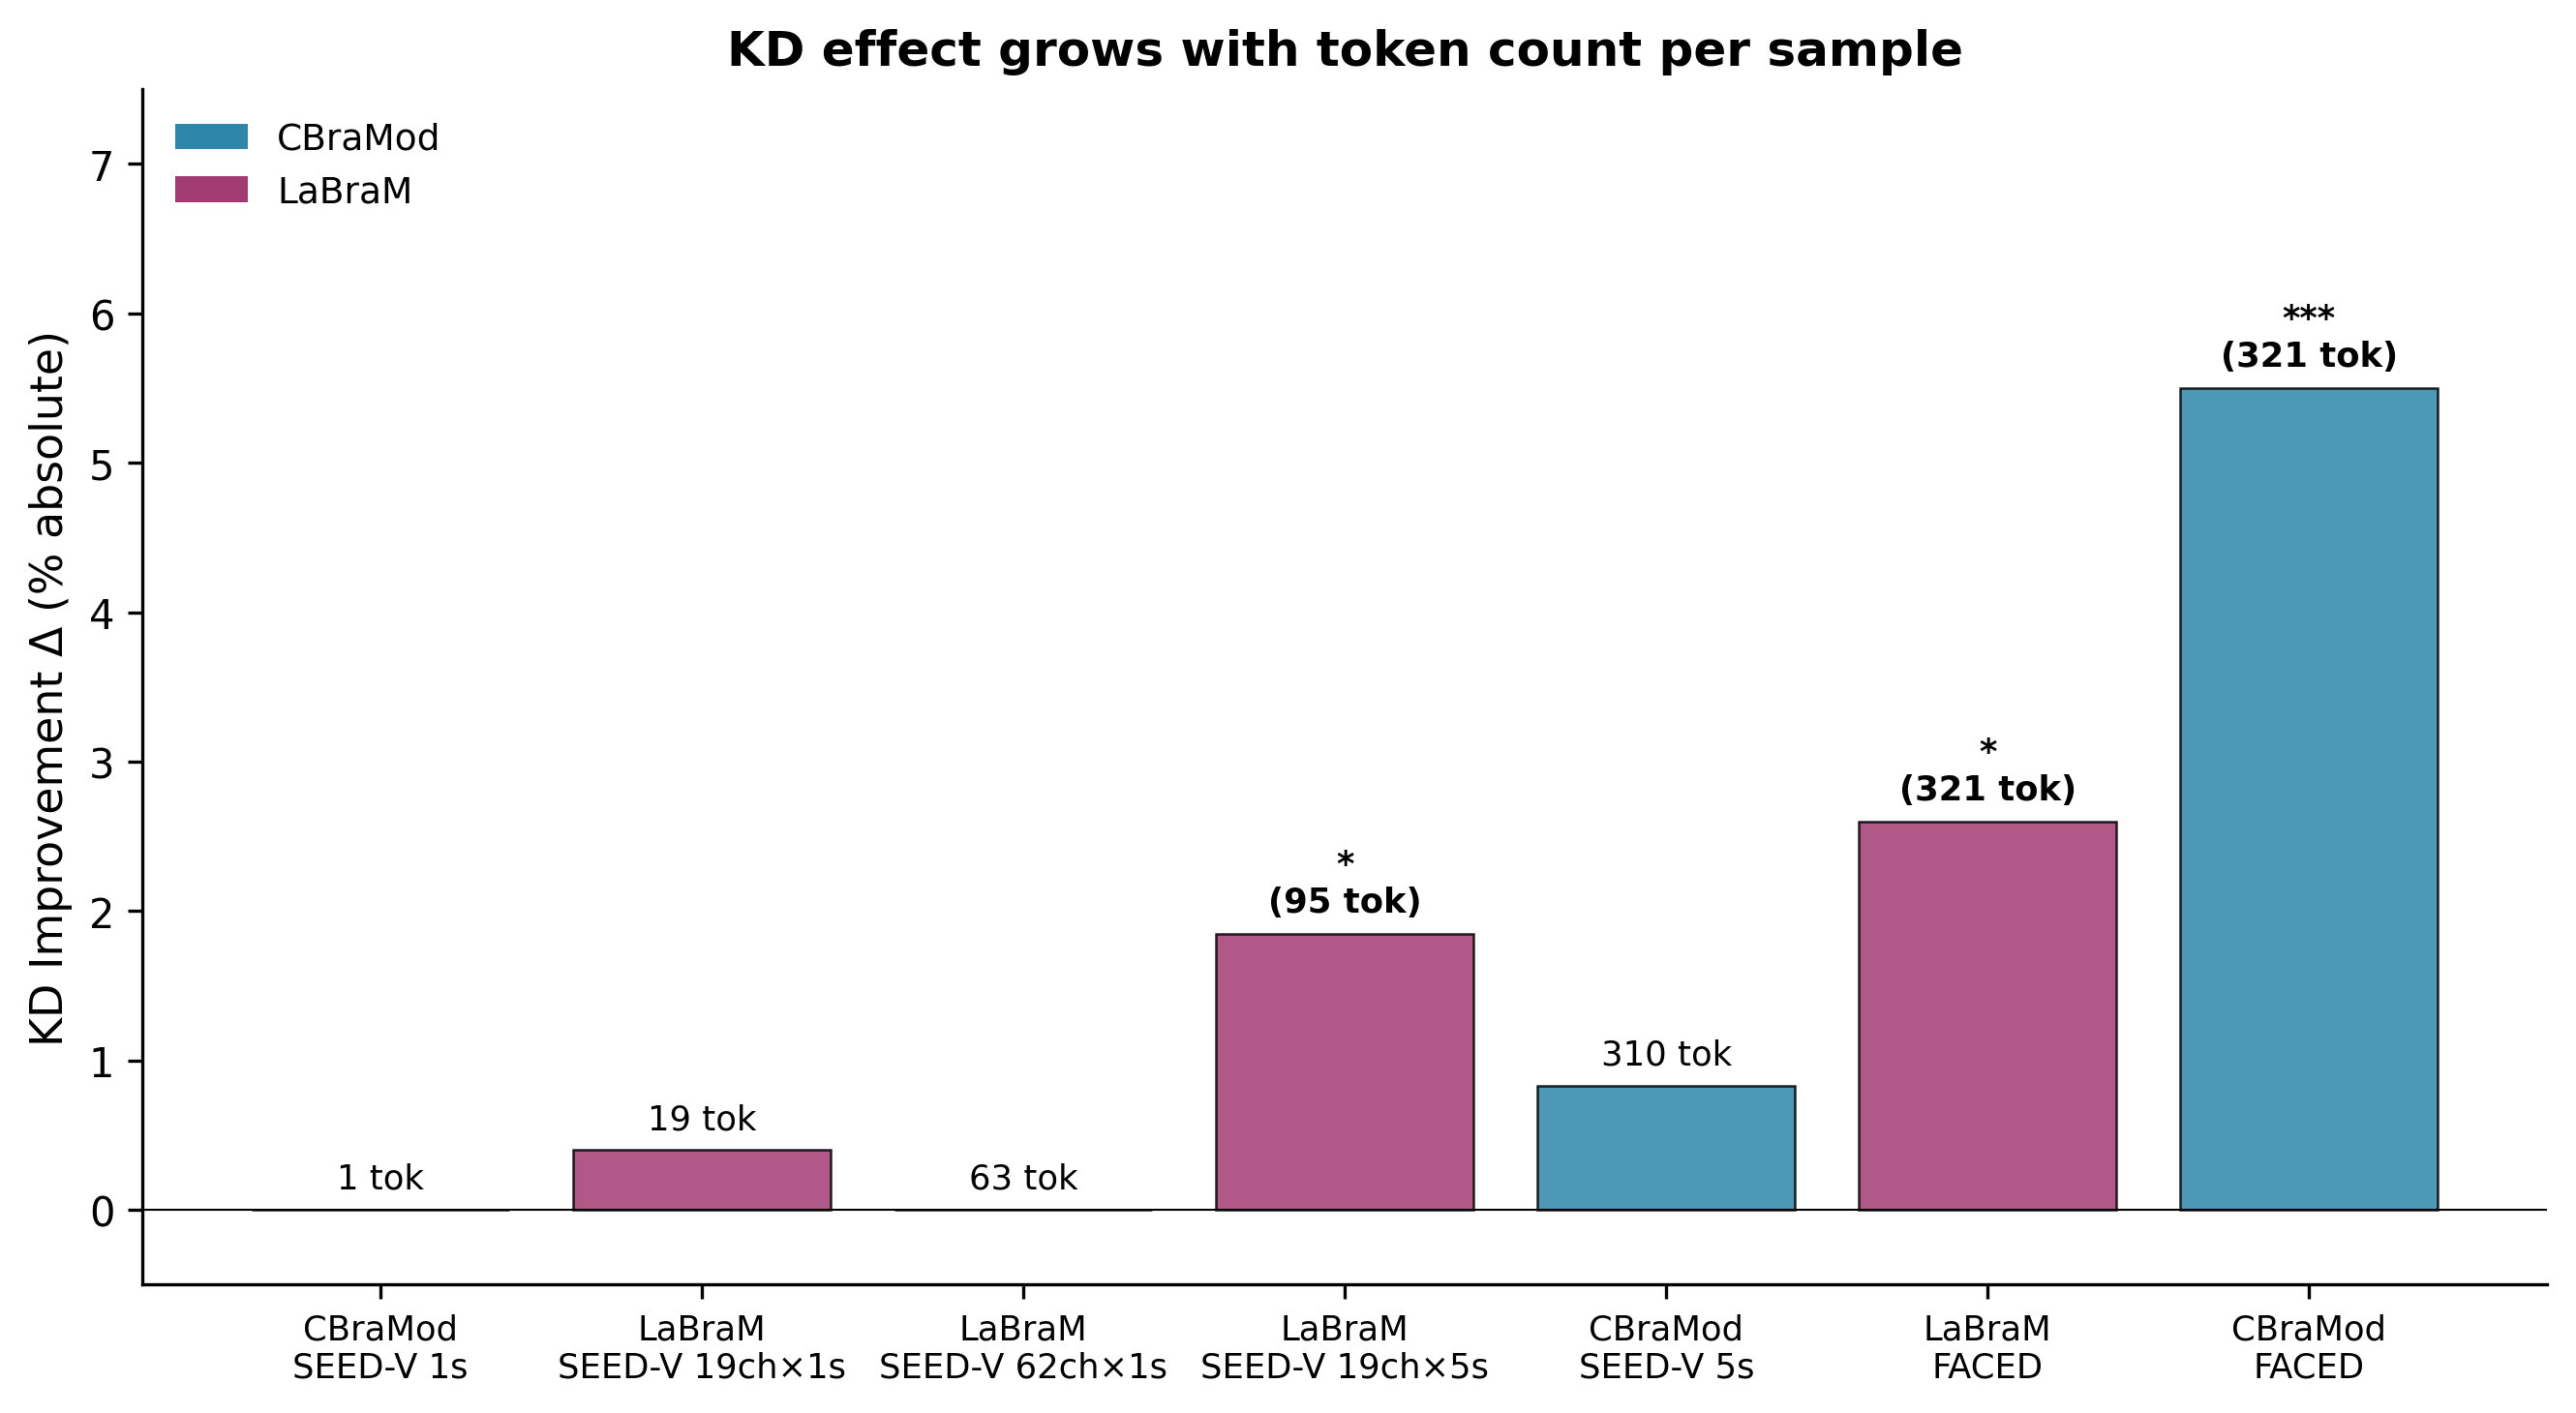
\includegraphics[width=0.95\linewidth]{figs/fig_token_threshold.png}
    \caption{KD improvement $\Delta$ as a function of token count per sample across multiple configurations. Within a fixed channel selection, the KD effect grows monotonically with the number of spatial-temporal tokens, ranging from a positive trend at small token counts to $+5.2\%$ at $\sim$320 tokens. Significance markers: $*$ paired $t$-test $p < 0.05$, $***$ $p < 0.001$, ``CI$>$0'' bootstrap 95\% CI excludes zero.}
    \label{fig:token_threshold}
\end{figure}

A natural question for any KD-based method is whether the supervisory signal interacts with input granularity. We investigate this by varying both the time window length (1\,s vs.\ 5\,s) and channel subset (full 62-channel SEED-V vs.\ standard 19-channel 10--20 montage~\cite{ten_twenty_montage}) on SEED-V, and comparing against the FACED setting (321 tokens per sample). \cref{fig:token_threshold} summarizes the relationship.

Two regularities emerge. First, \emph{within} a fixed channel selection, more temporal patches yield a larger and more reliable KD effect---LaBraM 19-channel SEED-V improves from a positive trend at 1\,s to $+1.85\%$ ($p = 0.037$) at 5\,s; CBraMod 62-channel SEED-V at 5\,s shows $\Delta = +0.36\%$ with bootstrap 95\% CI $[+0.0001, +0.0074]$. Second, FACED's $\sim$321 tokens per sample yields the largest KD effects ($+5.2\%$ on CBraMod, $+2.6\%$ on LaBraM). Third, when we attempted to apply the framework to EEG-DINO~\cite{wang2025eegdino}---an EEG foundation model whose default SEED-V preprocessing produces only $\sim$20 tokens per sample---KD, contrastive, and adapter extensions were all statistically flat ($|\Delta| \leq 0.003$ across 14 independent configurations; detailed in \cref{sec:supp_eegdino}), confirming that the token-count requirement is backbone-agnostic rather than a property of CBraMod alone. These results suggest a practical guideline: applying \ours\ to a new EEG dataset benefits from input preprocessing that yields a sufficient number of spatial-temporal tokens per training sample.

\begin{table}[!t]
\caption{Cross-architecture $\times$ cross-dataset matrix (FACED 9-class, SEED-V 5-class). \ours\ (aug + KD recipe) applied to CBraMod wins SEED-V; applied to EMOD it wins FACED. Each backbone dominates the dataset whose labels most closely match its pretraining objective---CBraMod was pretrained on TUEG (general) while EMOD was pretrained with valence/arousal contrastive objectives on non-SEED-V emotion datasets.}
\small
\centering
\begin{tabular}{lcc}
\toprule
Backbone & FACED (9c, B.Acc) & SEED-V (5c, B.Acc) \\
\midrule
CBraMod + \ours\ & $0.628 \pm 0.004$ & $\mathbf{0.417 \pm 0.001}$ \\
EMOD + \ours\ & $\mathbf{0.642 \pm 0.007}$ & $0.374 \pm 0.008$ \\
\midrule
CBraMod paper~\cite{wang2025cbramod} & $0.551$ & $0.409$ \\
EMOD paper~\cite{emod2026} & $0.629$ & --- \\
\bottomrule
\end{tabular}
\label{tab:cross_arch_dataset}
\end{table}

\cref{tab:cross_arch_dataset} summarizes the cross-architecture $\times$ cross-dataset matrix: our recipe improves both backbones over their published numbers but does \emph{not} invert the backbone-specific dataset preferences. CBraMod, pretrained on general EEG (TUEG), dominates SEED-V ($0.417$ vs.\ EMOD's $0.374$). EMOD, pretrained with explicit valence--arousal contrastive objectives on DEAP/AMIGOS/SEEDIV/SEEDVII, dominates FACED ($0.642$ vs.\ CBraMod's $0.628$) but fails to transfer to SEED-V's 5-class structure even when we match its native 5-second window length (\cref{sec:supp_emod_seedv}). This pattern argues that the aug$+$KD recipe improves whatever backbone it is paired with, but it does not override a fundamental mismatch between the pretraining data distribution and the downstream task structure.

\noindent\textbf{Extending the recipe beyond emotion: a component dissociation.} To test how far the recipe generalizes beyond emotion tasks, we apply the CBraMod + \ours\ pipeline to two additional CBraMod benchmark tasks: MentalArithmetic (2-class stress detection) and PhysioNet-MI (4-class motor imagery). Full details are in \cref{sec:supp_binary,sec:supp_physio}. On MentalArithmetic, our baseline replicates the paper's $0.726$ within $1.1\%$ ($0.715 \pm 0.020$) and the augmentation recipe then lifts it to $\mathbf{0.734 \pm 0.027}$, crossing above the paper target ($+0.019$ over our baseline). On PhysioNet-MI, our baseline replicates the paper's $0.5138$ within $0.7\%$ ($0.5069 \pm 0.015$), but augmentation is null ($+0.001$, $p=0.92$) while \textbf{KD alone hits the paper reference exactly} ($0.5139 \pm 0.024$, $+0.007$ over baseline). This dissociation cleanly separates the two recipe components: the augmentation is emotion-specialized---temporal jitter destroys the event-related desynchronization (ERD/ERS) timing that motor imagery labels depend on---while the fixed-prototype KD term is task-general and transfers across emotion and non-emotion multi-class tasks. On binary tasks (Mumtaz2016, MentalArithmetic), KD adds no further benefit because orthogonal 2-class prototypes encode no non-trivial geometry beyond what BCE already learns. We therefore do not claim universal recipe transfer; the \ours\ recipe is a decomposable pair of regularizers with complementary regimes of applicability.

\subsection{Augmentation Ablation}
\label{sec:aug_ablation}
\vspace{-1mm}

\begin{table}% [12]{r}{0.48\textwidth}
  \centering
  \vspace{-5mm}
  \caption{Augmentation drop-one-out on FACED. Temporal jitter is the only critical component.}
  \small
  \begin{tabular}{lcc}
  \toprule
  Config & B.Acc & $\Delta$ \\
  \midrule
  Full aug (all 4) & 0.609 & --- \\
  Drop noise & 0.609 & $+$0.0\% \\
  Drop dropout & 0.613 & $+$0.4\% \\
  Drop scaling & 0.611 & $+$0.2\% \\
  \textbf{Drop jitter} & \textbf{0.569} & $\mathbf{-3.9\%}$ \\
  \bottomrule
  \end{tabular}
  \label{tab:aug_ablation}
\end{table}

\cref{tab:aug_ablation} shows that temporal jitter is the single indispensable augmentation. Removing it drops performance by $-3.9\%$ (back to baseline level), while removing any other augmentation has negligible or even slightly positive effect. This finding has a biological interpretation: small temporal shifts ($\pm$20 samples at 200\,Hz $= \pm$100\,ms) force the model to learn timing-invariant representations, which is essential for EEG where neural response onset varies across trials and subjects.

\subsection{KD Loss Ablation}
\label{sec:kd_ablation}
\vspace{-1mm}

\begin{wraptable}[14]{r}{0.48\textwidth}
  \centering
  \vspace{-5mm}
  \caption{KD hyperparameter sensitivity on FACED (5 seeds each). Augmentation probability has the largest effect.}
  \small
  \begin{tabular}{lcc}
  \toprule
  Parameter & Value & B.Acc \\
  \midrule
  $\lambda = 0.05$ & & 0.620 \\
  $\lambda = 0.10$ (default) & & 0.621 \\
  $\lambda = 0.20$ & & 0.616 \\
  $\lambda = 0.50$ & & 0.610 \\
  \midrule
  $\tau_t = 0.05$ & & 0.622 \\
  $\tau_t = 0.10$ (default) & & 0.621 \\
  $\tau_t = 0.20$ & & 0.619 \\
  \midrule
  $p_{\text{aug}} = 0.4$ & & 0.614 \\
  $p_{\text{aug}} = 0.5$ (default) & & 0.621 \\
  $\mathbf{p_{\text{aug}} = 0.6}$ & & \textbf{0.627} \\
  \bottomrule
  \end{tabular}
  \label{tab:kd_ablation}
\end{wraptable}

We sweep KD hyperparameters across 40 tasks (\cref{tab:kd_ablation}). $\lambda$ is robust in $[0.05, 0.10]$ but degrades sharply above $0.20$, indicating that the KD signal should complement rather than dominate the CE loss. Sharper teacher temperature ($\tau_t = 0.05$) marginally helps. Augmentation probability has the largest effect, with $p_{\text{aug}} = 0.6$ yielding the best result.

\subsection{Baseline Comparison: What Does KD Add?}
\label{sec:baseline_ablation}
\vspace{-1mm}

\begin{table}[!t]
\caption{Controlled comparison on FACED (5 seeds each). All methods use the same 3-layer BN projection head and augmentation to isolate the effect of the loss function and teacher signal.}
\small
\centering
\setlength{\tabcolsep}{5pt}
\begin{tabular}{lccc}
\toprule
Method & B.Acc & $\kappa$ & vs Aug \\
\midrule
CBraMod baseline & 0.572 & 0.516 & $-3.7\%$ \\
Aug only & 0.609 & 0.557 & --- \\
SupCon + aug & 0.611 & 0.560 & $+0.2\%$ \\
VA + aug & 0.611 & 0.559 & $+0.2\%$ \\
\midrule
\multicolumn{4}{l}{\textit{Same 3L-BN projection head:}} \\
One-hot KD + 3L-BN & 0.616 & 0.565 & $+0.7\%$ \\
Random Gaussian KD + 3L-BN & 0.619 & 0.568 & $+1.0\%$ \\
InfoNCE + 3L-BN & 0.614 & 0.563 & $+0.5\%$ \\
SBERT KD + 3L-BN & 0.623 & 0.572 & $+1.4\%$ \\
LLM \emph{logit} KD + 3L-BN & 0.606 & 0.553 & $-0.3\%$ \\
Adapter64 + InfoNCE & 0.620 & 0.569 & $+1.1\%$ \\
\rowcolor{blond}
\textbf{LLM \emph{hidden-state} KD + 3L-BN (ours)} & \textbf{0.627} & \textbf{0.577} & $\mathbf{+1.8\%}$ \\
\bottomrule
\end{tabular}
\label{tab:baselines}
\end{table}

\cref{tab:baselines} isolates the contribution of the LLM teacher signal. With the same 3L-BN projection head, LLM hidden-state KD ($0.627$) beats InfoNCE ($0.614$) by $+1.3\%$ and SBERT-text KD ($0.623$) by $+0.4\%$. Critically, we also include an \emph{LLM logit KD} baseline where the teacher distribution comes from the LLM's classification probabilities (the LLM is prompted with the emotion-laden stories and we read off its 9-way emotion predictions) rather than from the internal hidden-state geometry. Logit KD yields $0.606$---\emph{worse} than aug-only---while hidden-state KD yields $0.627$ ($\Delta = +2.1\%$, paired $t = 4.08$, $p = 0.015$, bootstrap 95\% CI $[+1.05\%, +2.77\%]$). This is strong evidence that the value of LLM-guided supervision comes from the \emph{relational geometry} encoded in hidden states, not from the LLM's black-box classification ability. SupCon ($0.611$) and direct valence--arousal regression ($0.611$) match aug-only at $\sim$$0.609$, indicating that generic contrastive losses do not add value beyond the augmentation pipeline.

\subsection{PEFT Analysis: Adapter64 on FACED}
\label{sec:adapter_ablation}
\vspace{-1mm}

\begin{figure}[!t]
    \centering
    \begin{subfigure}[b]{0.48\textwidth}
        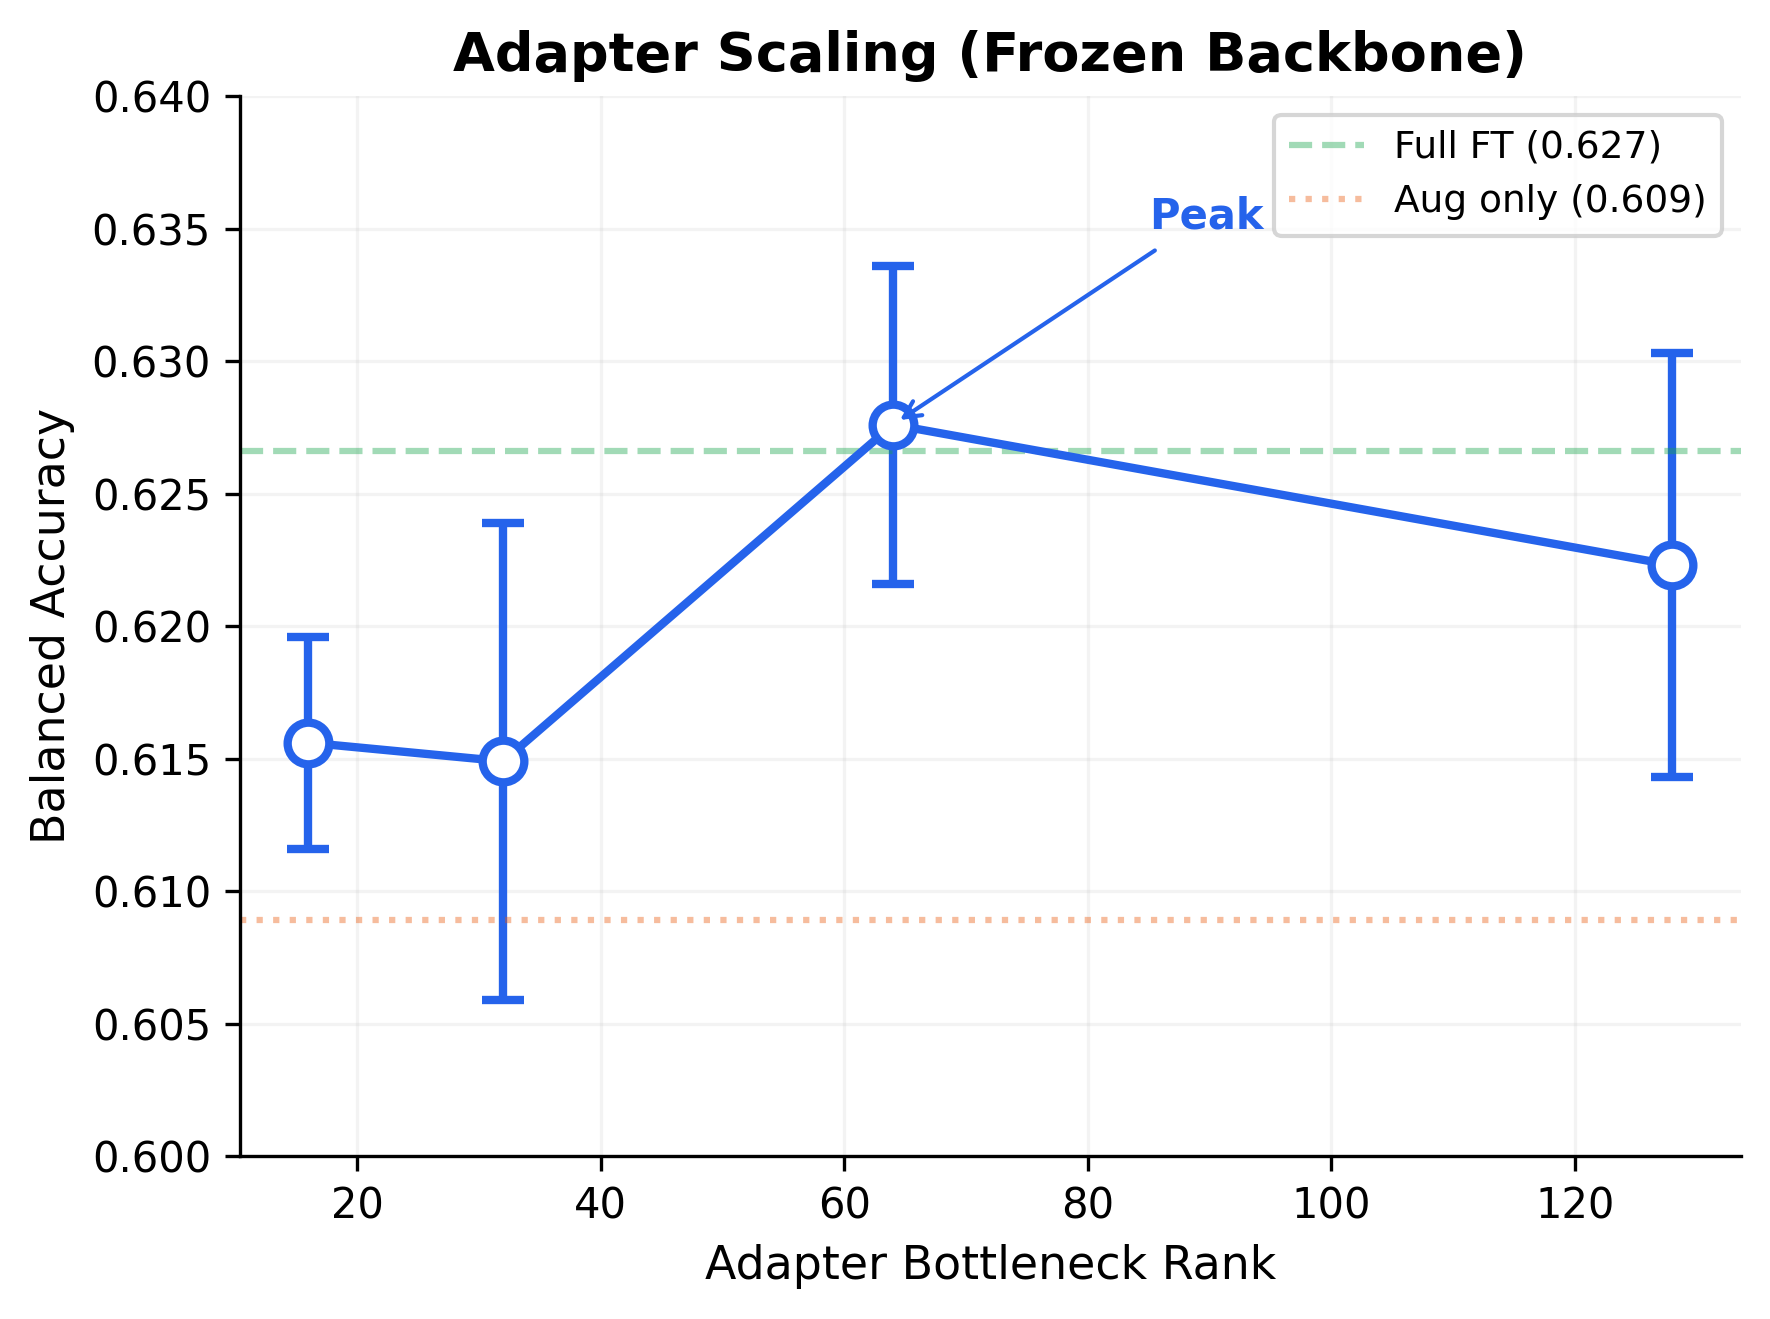
\includegraphics[width=\linewidth]{figs/adapter_scaling.png}
        \caption{Adapter scaling on FACED: peak at $r=64$.}
        \label{fig:adapter_scaling}
    \end{subfigure}
    \hfill
    \begin{subfigure}[b]{0.48\textwidth}
        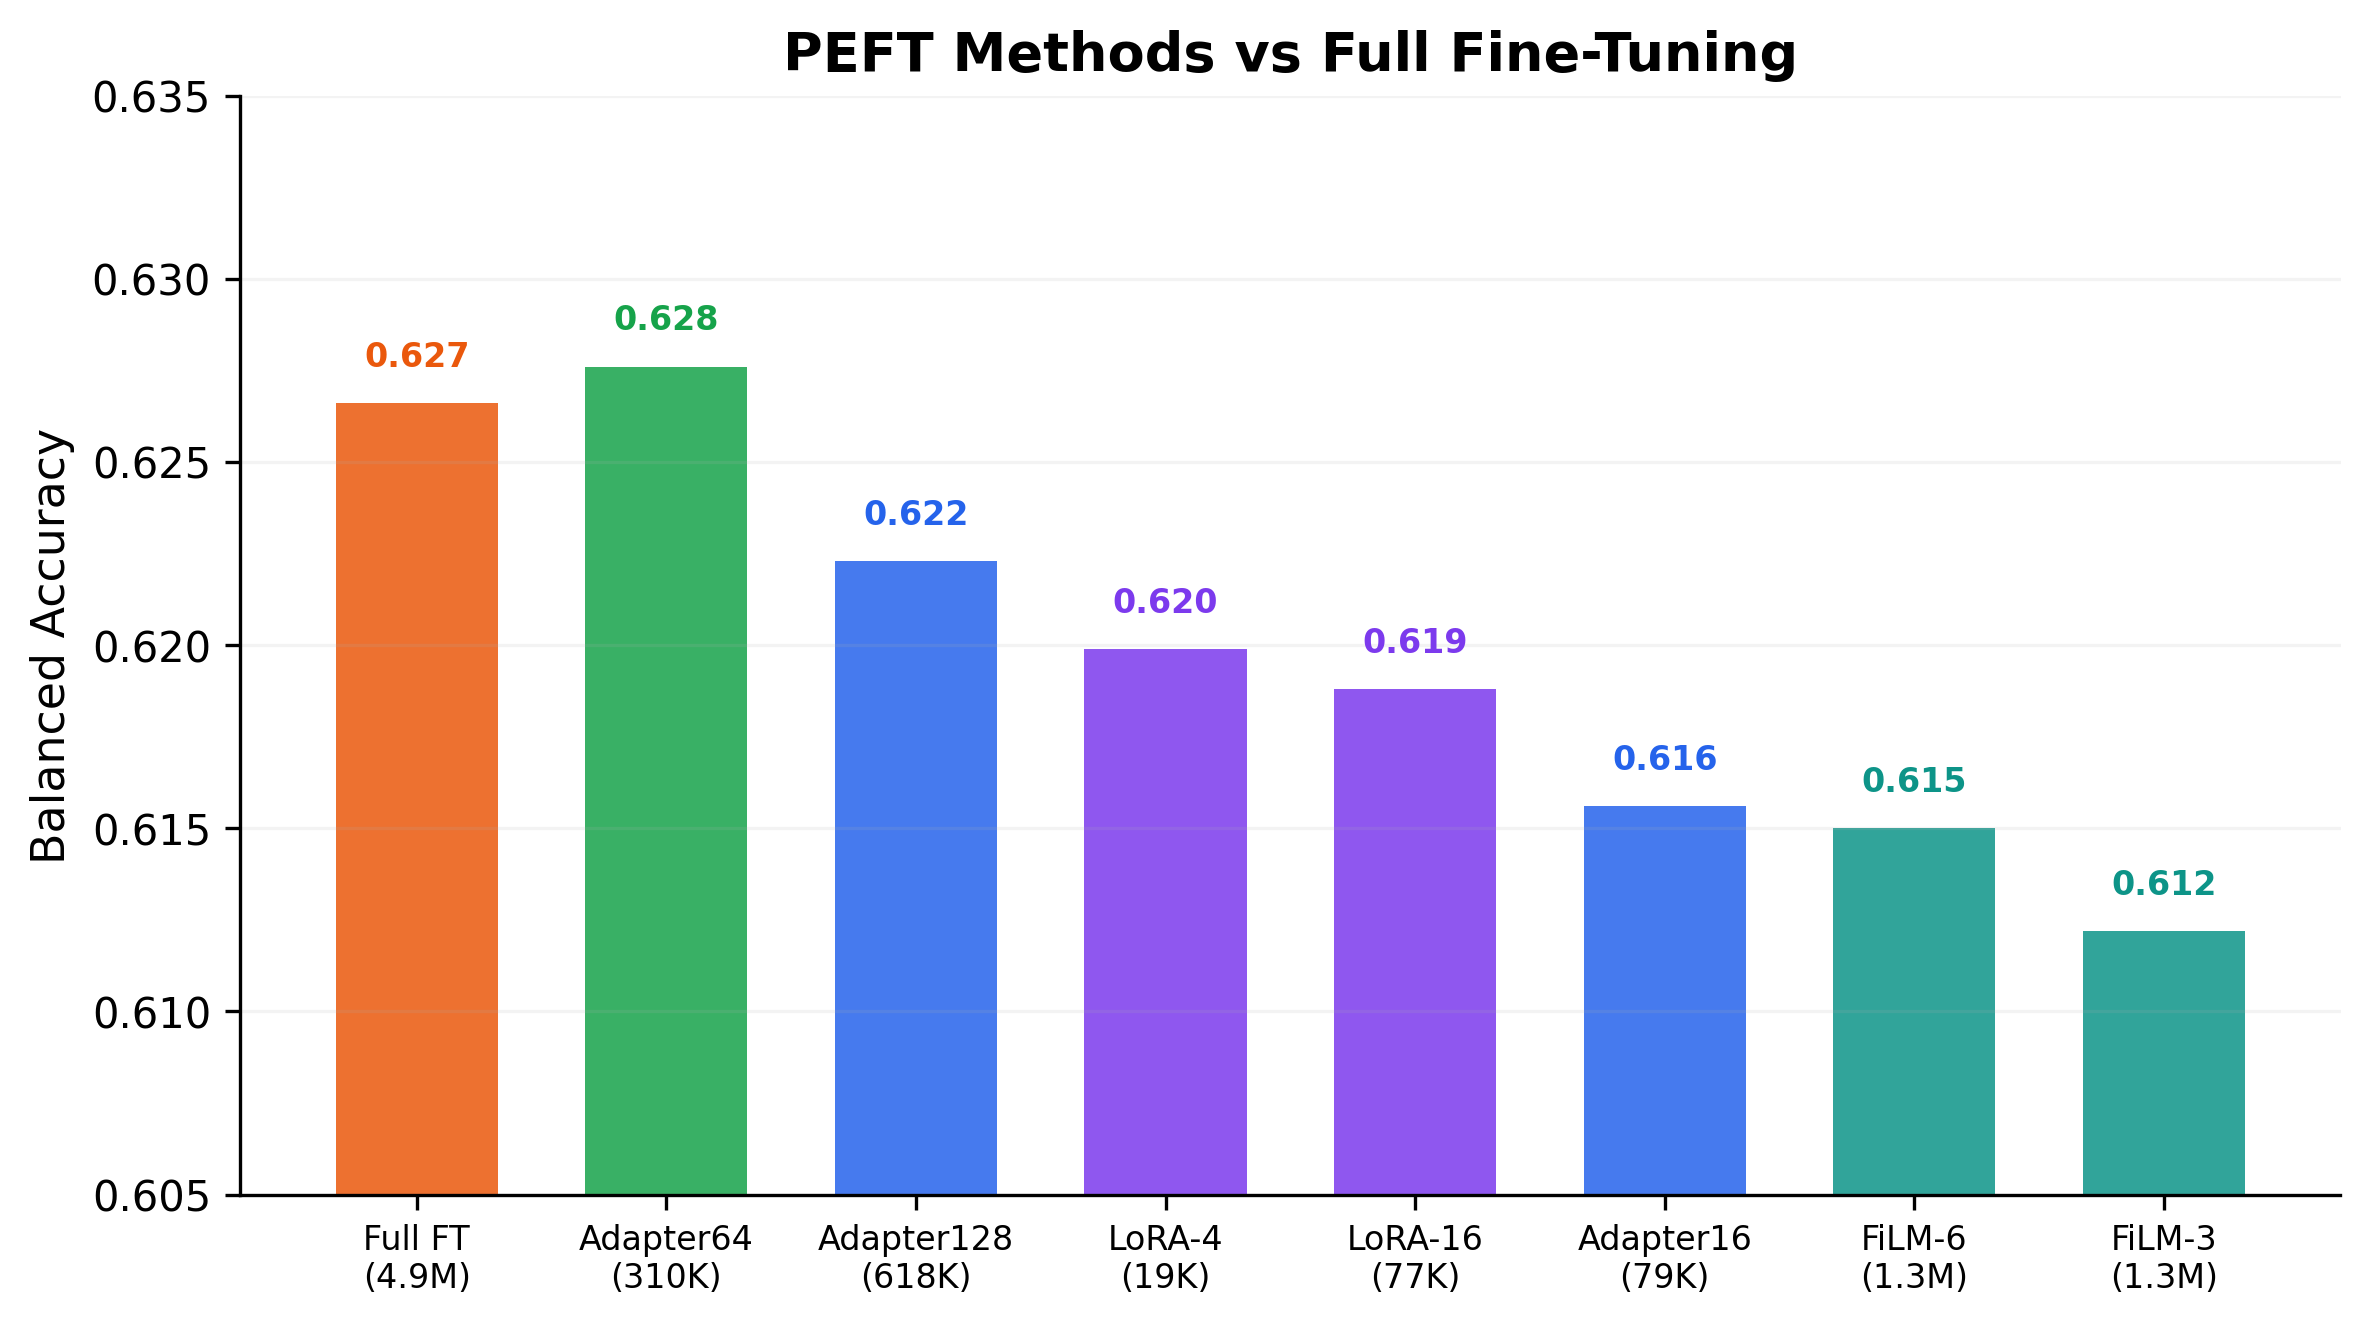
\includegraphics[width=\linewidth]{figs/peft_comparison.png}
        \caption{PEFT methods vs.\ full fine-tuning.}
        \label{fig:peft}
    \end{subfigure}
    \caption{(a) Adapter bottleneck scaling on FACED. Performance peaks at $r = 64$ ($0.628$), then decreases for $r = 128$ ($0.622$) due to overfitting with frozen backbone. (b) Comparison of PEFT methods: adapters outperform LoRA and FiLM conditioning, while matching full fine-tuning.}
    \label{fig:adapter_analysis}
\end{figure}

We systematically evaluate three PEFT approaches with frozen backbone: bottleneck adapters (rank 16/32/64/128), LoRA~\cite{hu2022lora} (rank 4/8/16), and FiLM conditioning~\cite{perez2018film} (3/6 modulation layers). The adapter scaling curve (\cref{fig:adapter_scaling}) shows a clear peak at $r=64$: $r=16$ ($0.616$) $\to$ $r=32$ ($0.615$) $\to$ $r=64$ ($\mathbf{0.628}$) $\to$ $r=128$ ($0.622$). LoRA achieves $\sim$$0.619$ across ranks (4/8/16), and FiLM ($0.612$--$0.615$) provides a complementary perspective. Training adapters with frozen backbone ($0.628$) outperforms unfreezing the backbone after adapter warmup ($0.615$), demonstrating that CBraMod's pretrained representations benefit from being preserved intact.

\noindent\textbf{Scope of the frozen-backbone property.} We tested whether the frozen-backbone PEFT strategy also applies to EMOD~\cite{emod2026} by freezing its axial-transformer backbone and training only the classifier and semantic projection head (\cref{sec:supp_emod_frozen}). Both aug and aug+KD variants collapsed to $0.432 \pm 0.02$---a $-0.21$ absolute drop from EMOD's full-FT score ($0.642$). The frozen-backbone strategy therefore does \emph{not} generalize across architectures: it succeeds with CBraMod (TUEG pretraining produces task-aligned EEG features) and fails with EMOD (V-A contrastive pretraining produces features that are not directly useful for FACED's 9-class categorical labels and require full fine-tuning to adapt).

\subsection{Error Pattern and LLM Emotion Geometry}
\label{sec:analysis}
\vspace{-1mm}

\begin{figure}[!t]
    \centering
    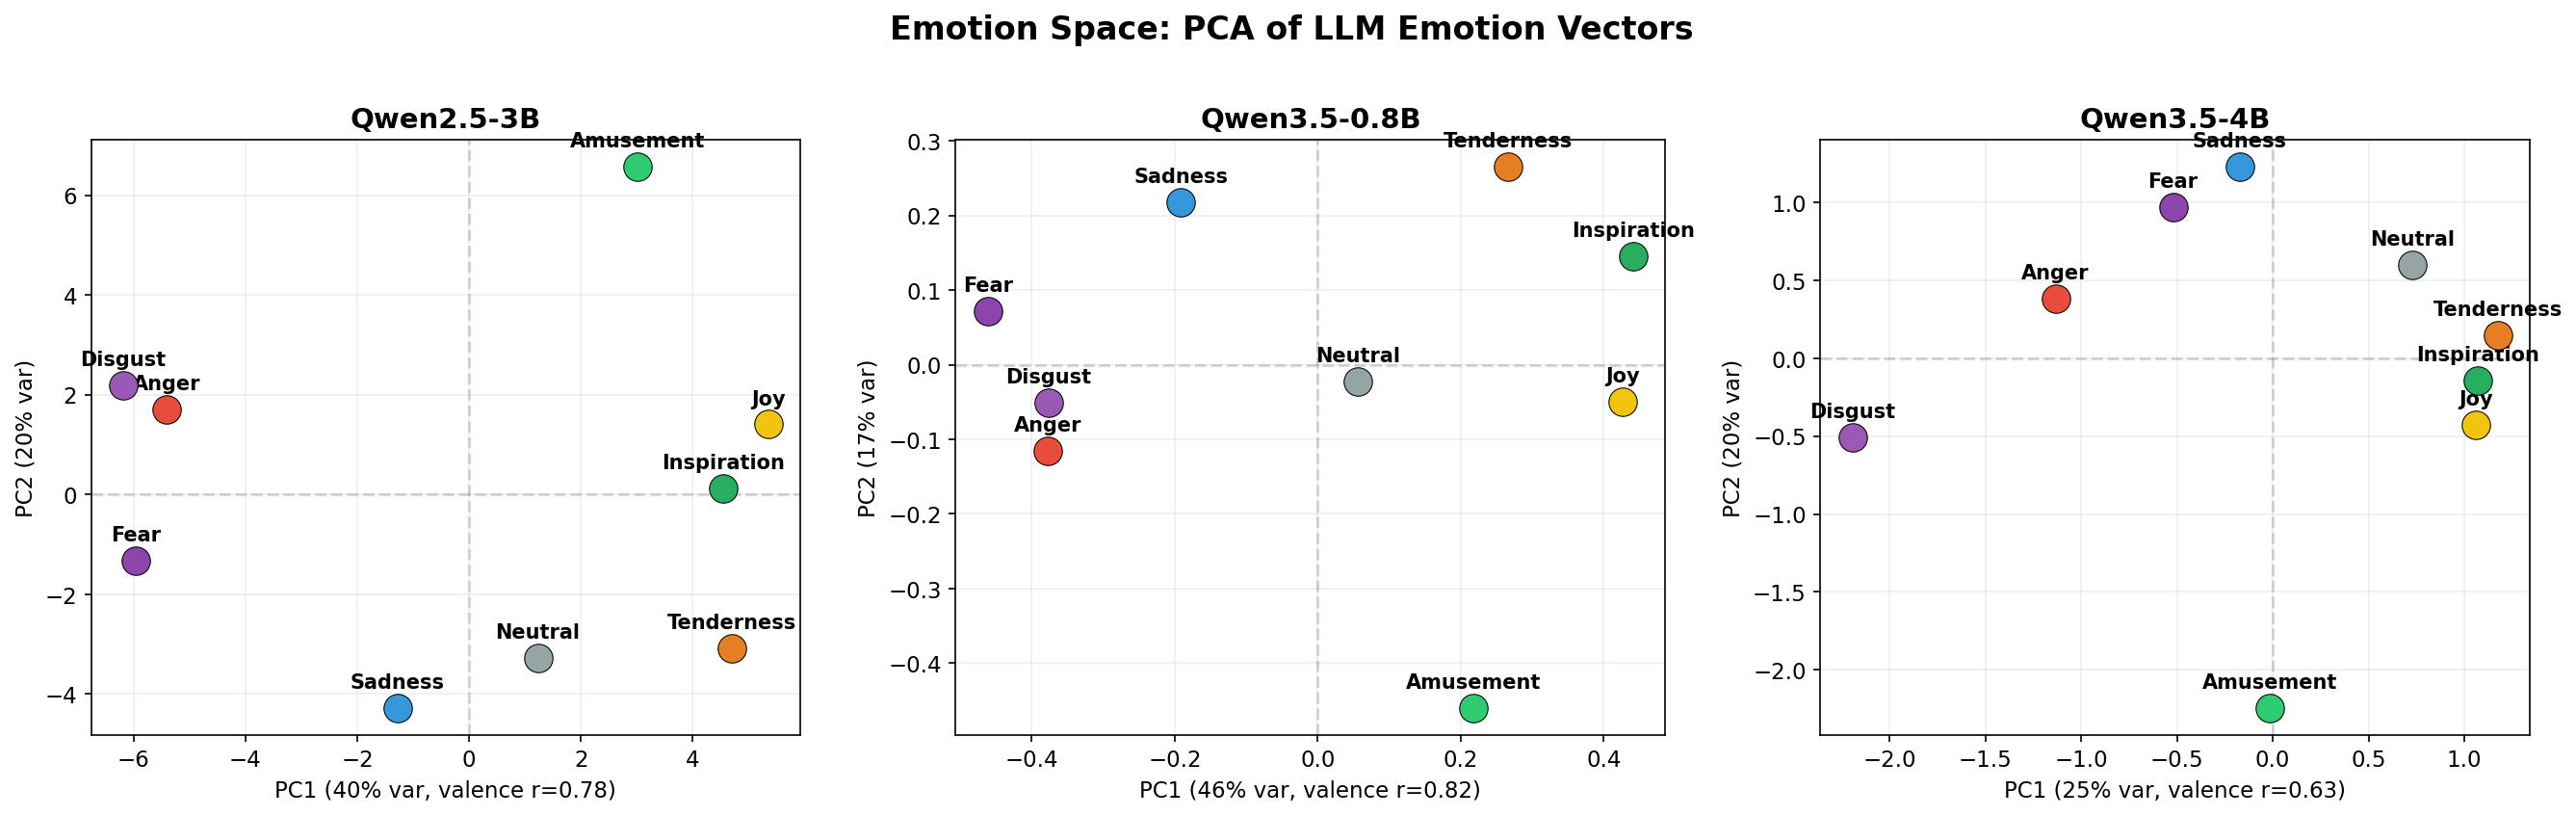
\includegraphics[width=\textwidth]{figs/fig1_pca_circumplex.png}
    \caption{PCA of Qwen2.5-0.5B emotion vectors recovers the full valence$\times$arousal circumplex~\cite{russell1980circumplex}. PC1 separates positive from negative valence; within the negative cluster, high-arousal emotions (anger, fear, disgust) separate from low-arousal sadness along PC2, mirroring the two-dimensional structure established in affective science.}
    \label{fig:pca}
\end{figure}

\begin{figure*}[!t]
    \centering
    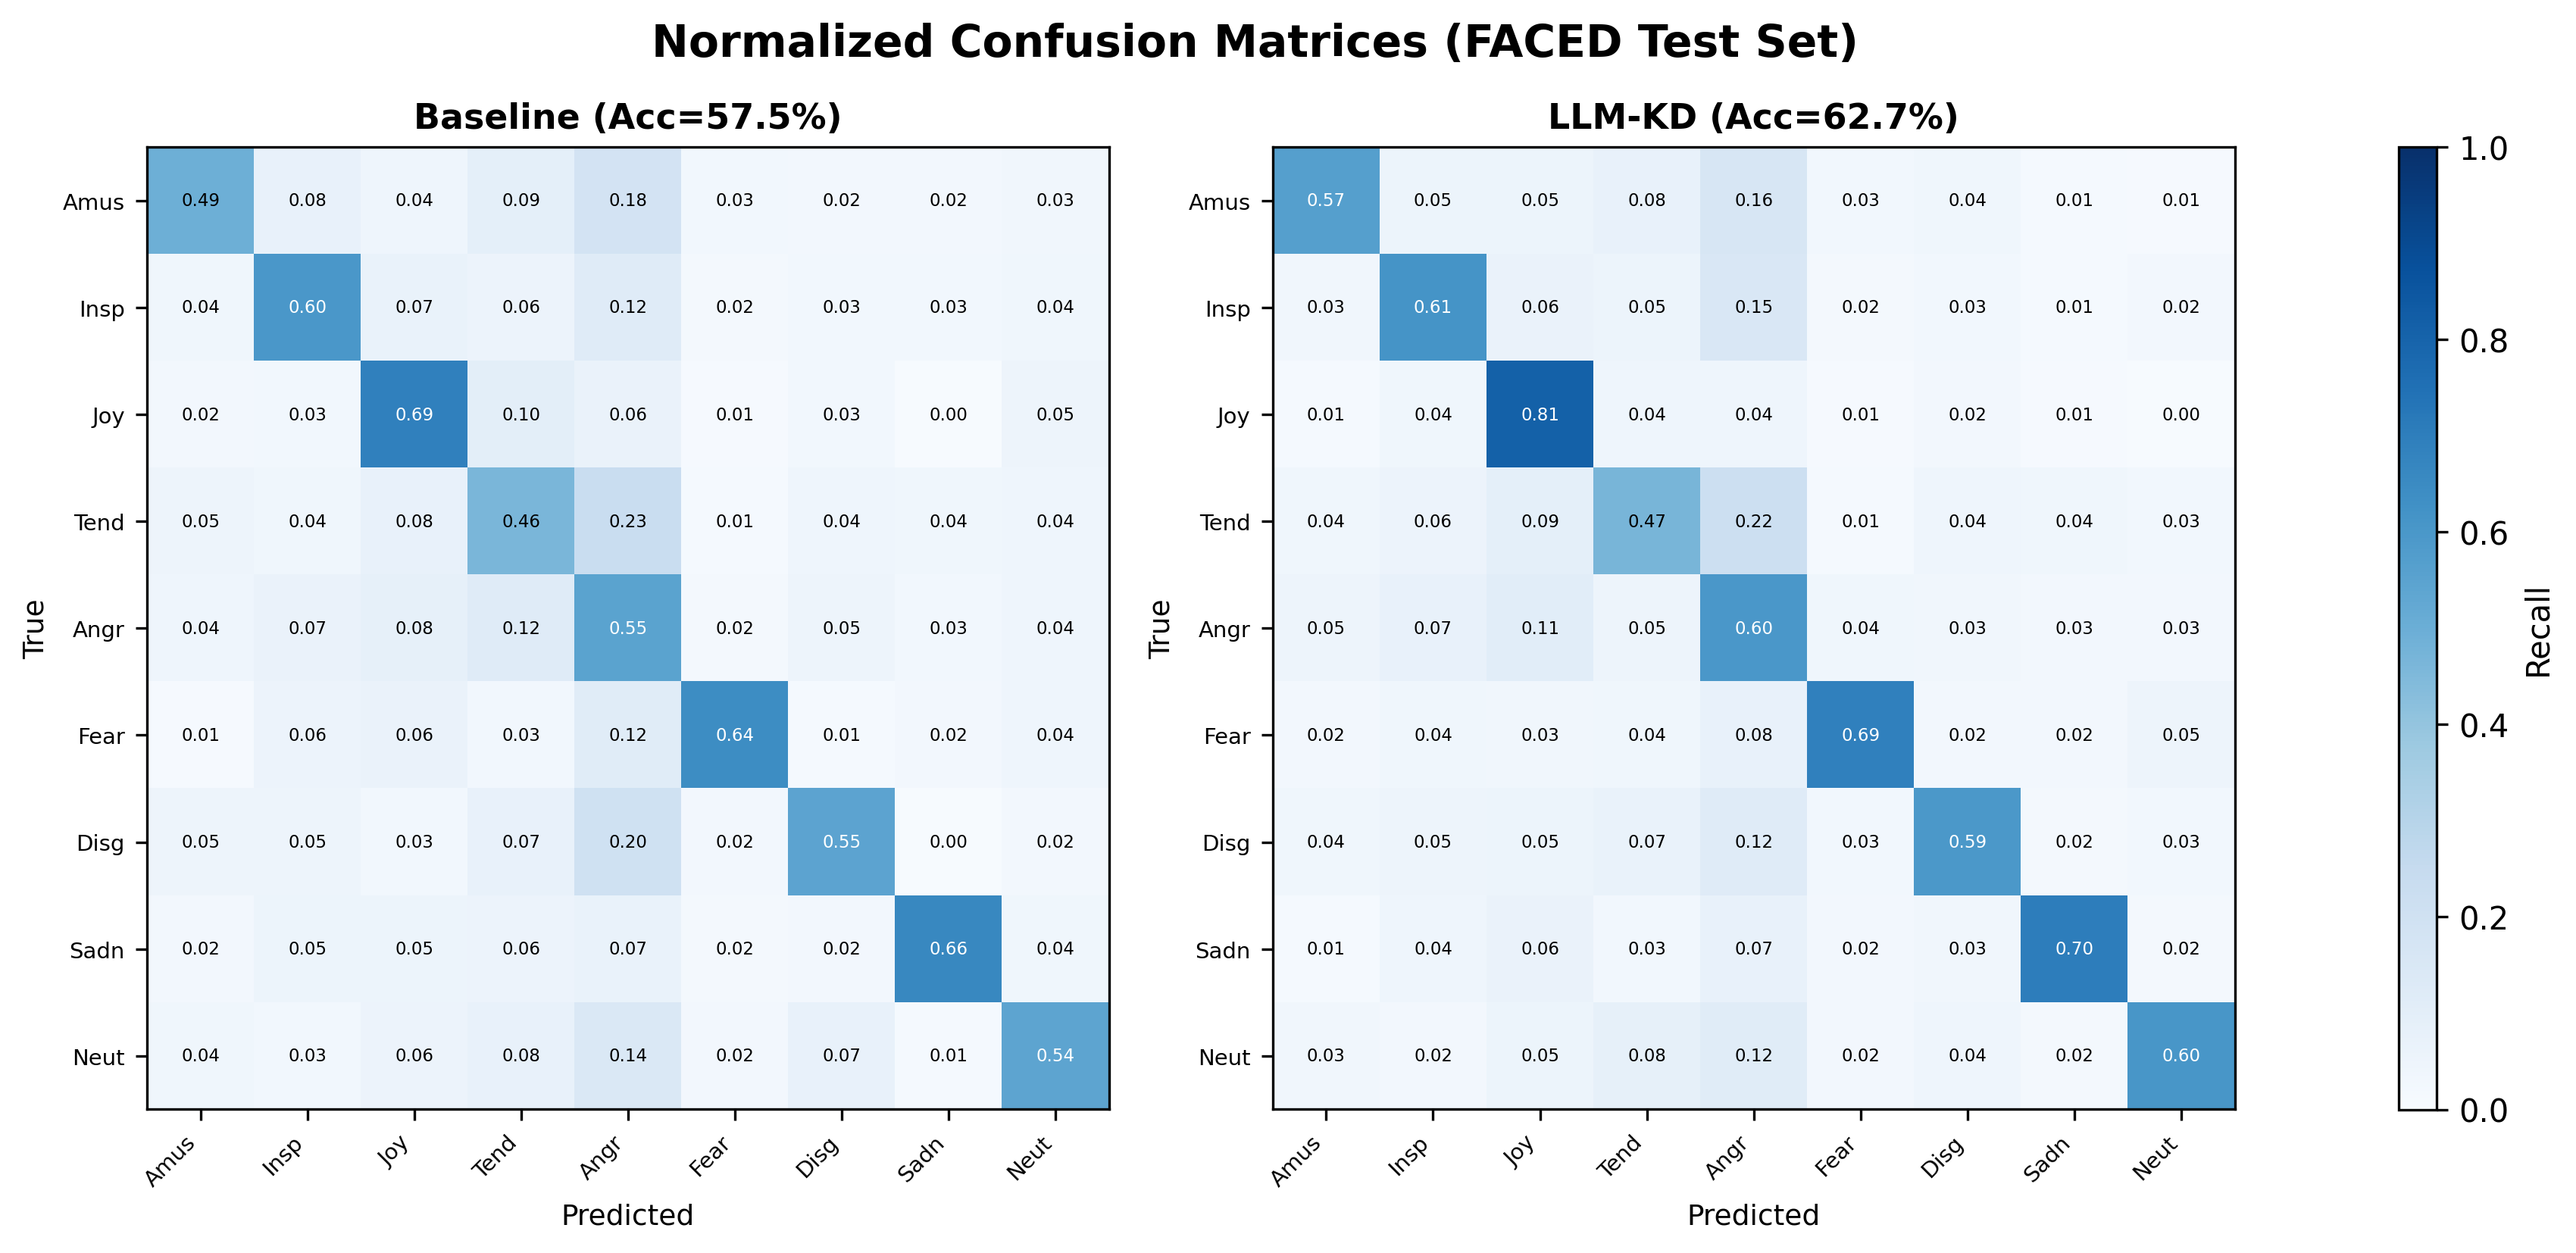
\includegraphics[width=\textwidth]{figs/confusion_matrices.png}
    \caption{Confusion matrices on FACED test set (seed 3407): CBraMod baseline (left, B.Acc $= 0.576$) vs.\ \ours KD (right, B.Acc $= 0.628$). Per-class recall improvements: Joy $+12.1\%$, Amusement $+7.2\%$, Neutral $+6.3\%$, Anger $+5.4\%$, Fear $+4.8\%$, Disgust $+4.8\%$, Sadness $+3.9\%$, Inspiration $+1.4\%$, Tenderness $+0.5\%$.}
    \label{fig:confusion}
\end{figure*}

\noindent\textbf{Error pattern.} EEG misclassification errors follow LLM semantic similarity (Spearman $r = 0.38$, $p = 3.4 \times 10^{-6}$). The effect is driven by negative-emotion confusions ($64.6\%$ of within-category errors, $p = 3.2 \times 10^{-13}$). Controls show that SBERT text descriptions ($r = 0.40$) are also strong predictors, while single-word embeddings and random vectors produce null results---indicating that the predictive structure lives in the LLM's full sentence-level representation, not in token-level word identities.

\noindent\textbf{Per-class improvement.} Confusion-matrix analysis (\cref{fig:confusion}) shows the largest gains on high-arousal positive emotions: joy ($+12.1\%$), amusement ($+7.2\%$), and on the high-arousal negative cluster: anger ($+5.4\%$), fear ($+4.8\%$), disgust ($+4.8\%$). Sadness, the only low-arousal negative emotion, shows a smaller gain ($+3.9\%$). This pattern is consistent with the LLM emotion geometry: the extracted vectors recover not just the valence axis but the full valence$\times$arousal circumplex, placing sadness apart from the high-arousal negative cluster. The KD loss exploits this two-dimensional structure, providing graded supervision that distinguishes both valence \emph{and} arousal.

\noindent\textbf{Per-subject analysis.} KD improves $87\%$ of subjects ($20/23$ in our test split), with mean balanced-accuracy gain of $+5.2\%$ and maximum $+11.7\%$ (subject 117). Per-subject gains are \emph{not} correlated with baseline accuracy (Pearson $r = -0.14$, $p = 0.51$), indicating the benefit is broadly distributed rather than concentrated on initially weak subjects. The sorted per-subject gain distribution is shown in \cref{fig:subject_benefit} (Supp.~\cref{sec:supp_per_subject}).

\subsection{LLM Scale and Cross-Family Universality}
\label{sec:llm_scale}
\vspace{-1mm}

\begin{figure}[!t]
    \centering
    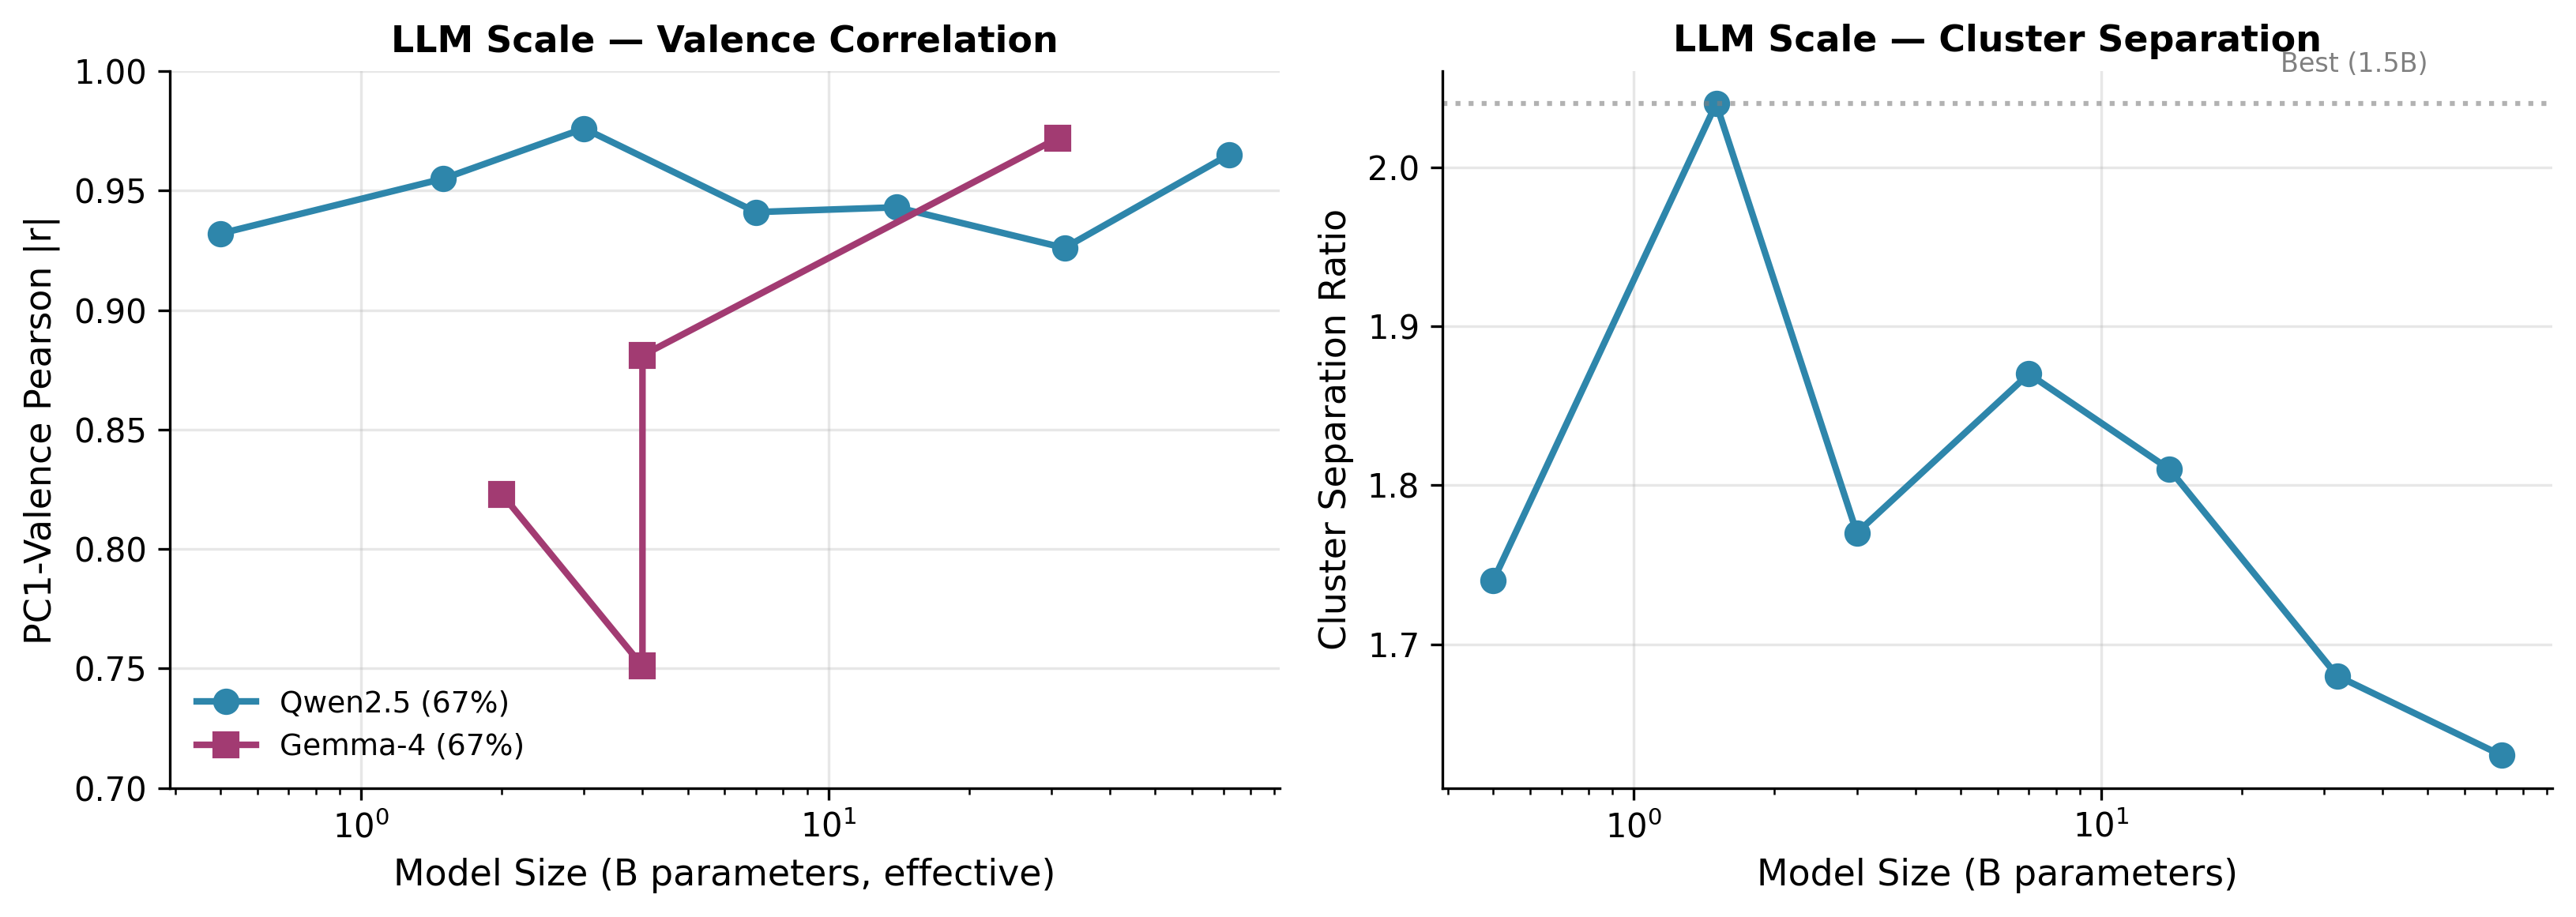
\includegraphics[width=0.96\linewidth]{figs/fig_llm_scale_dual.png}
    \caption{LLM scale analysis. \textbf{Left:} PC1--valence Pearson $|r|$ as a function of model size for Qwen2.5 and Gemma-4 families at the 67th-percentile layer. \textbf{Right:} Cluster separation ratio (inter-class vs intra-class distance) for Qwen sizes; this metric peaks at 1.5B ($2.04$)---the dimension that matters for KD soft-label informativeness.}
    \label{fig:llm_scale_dual}
\end{figure}

\begin{figure}[!t]
    \centering
    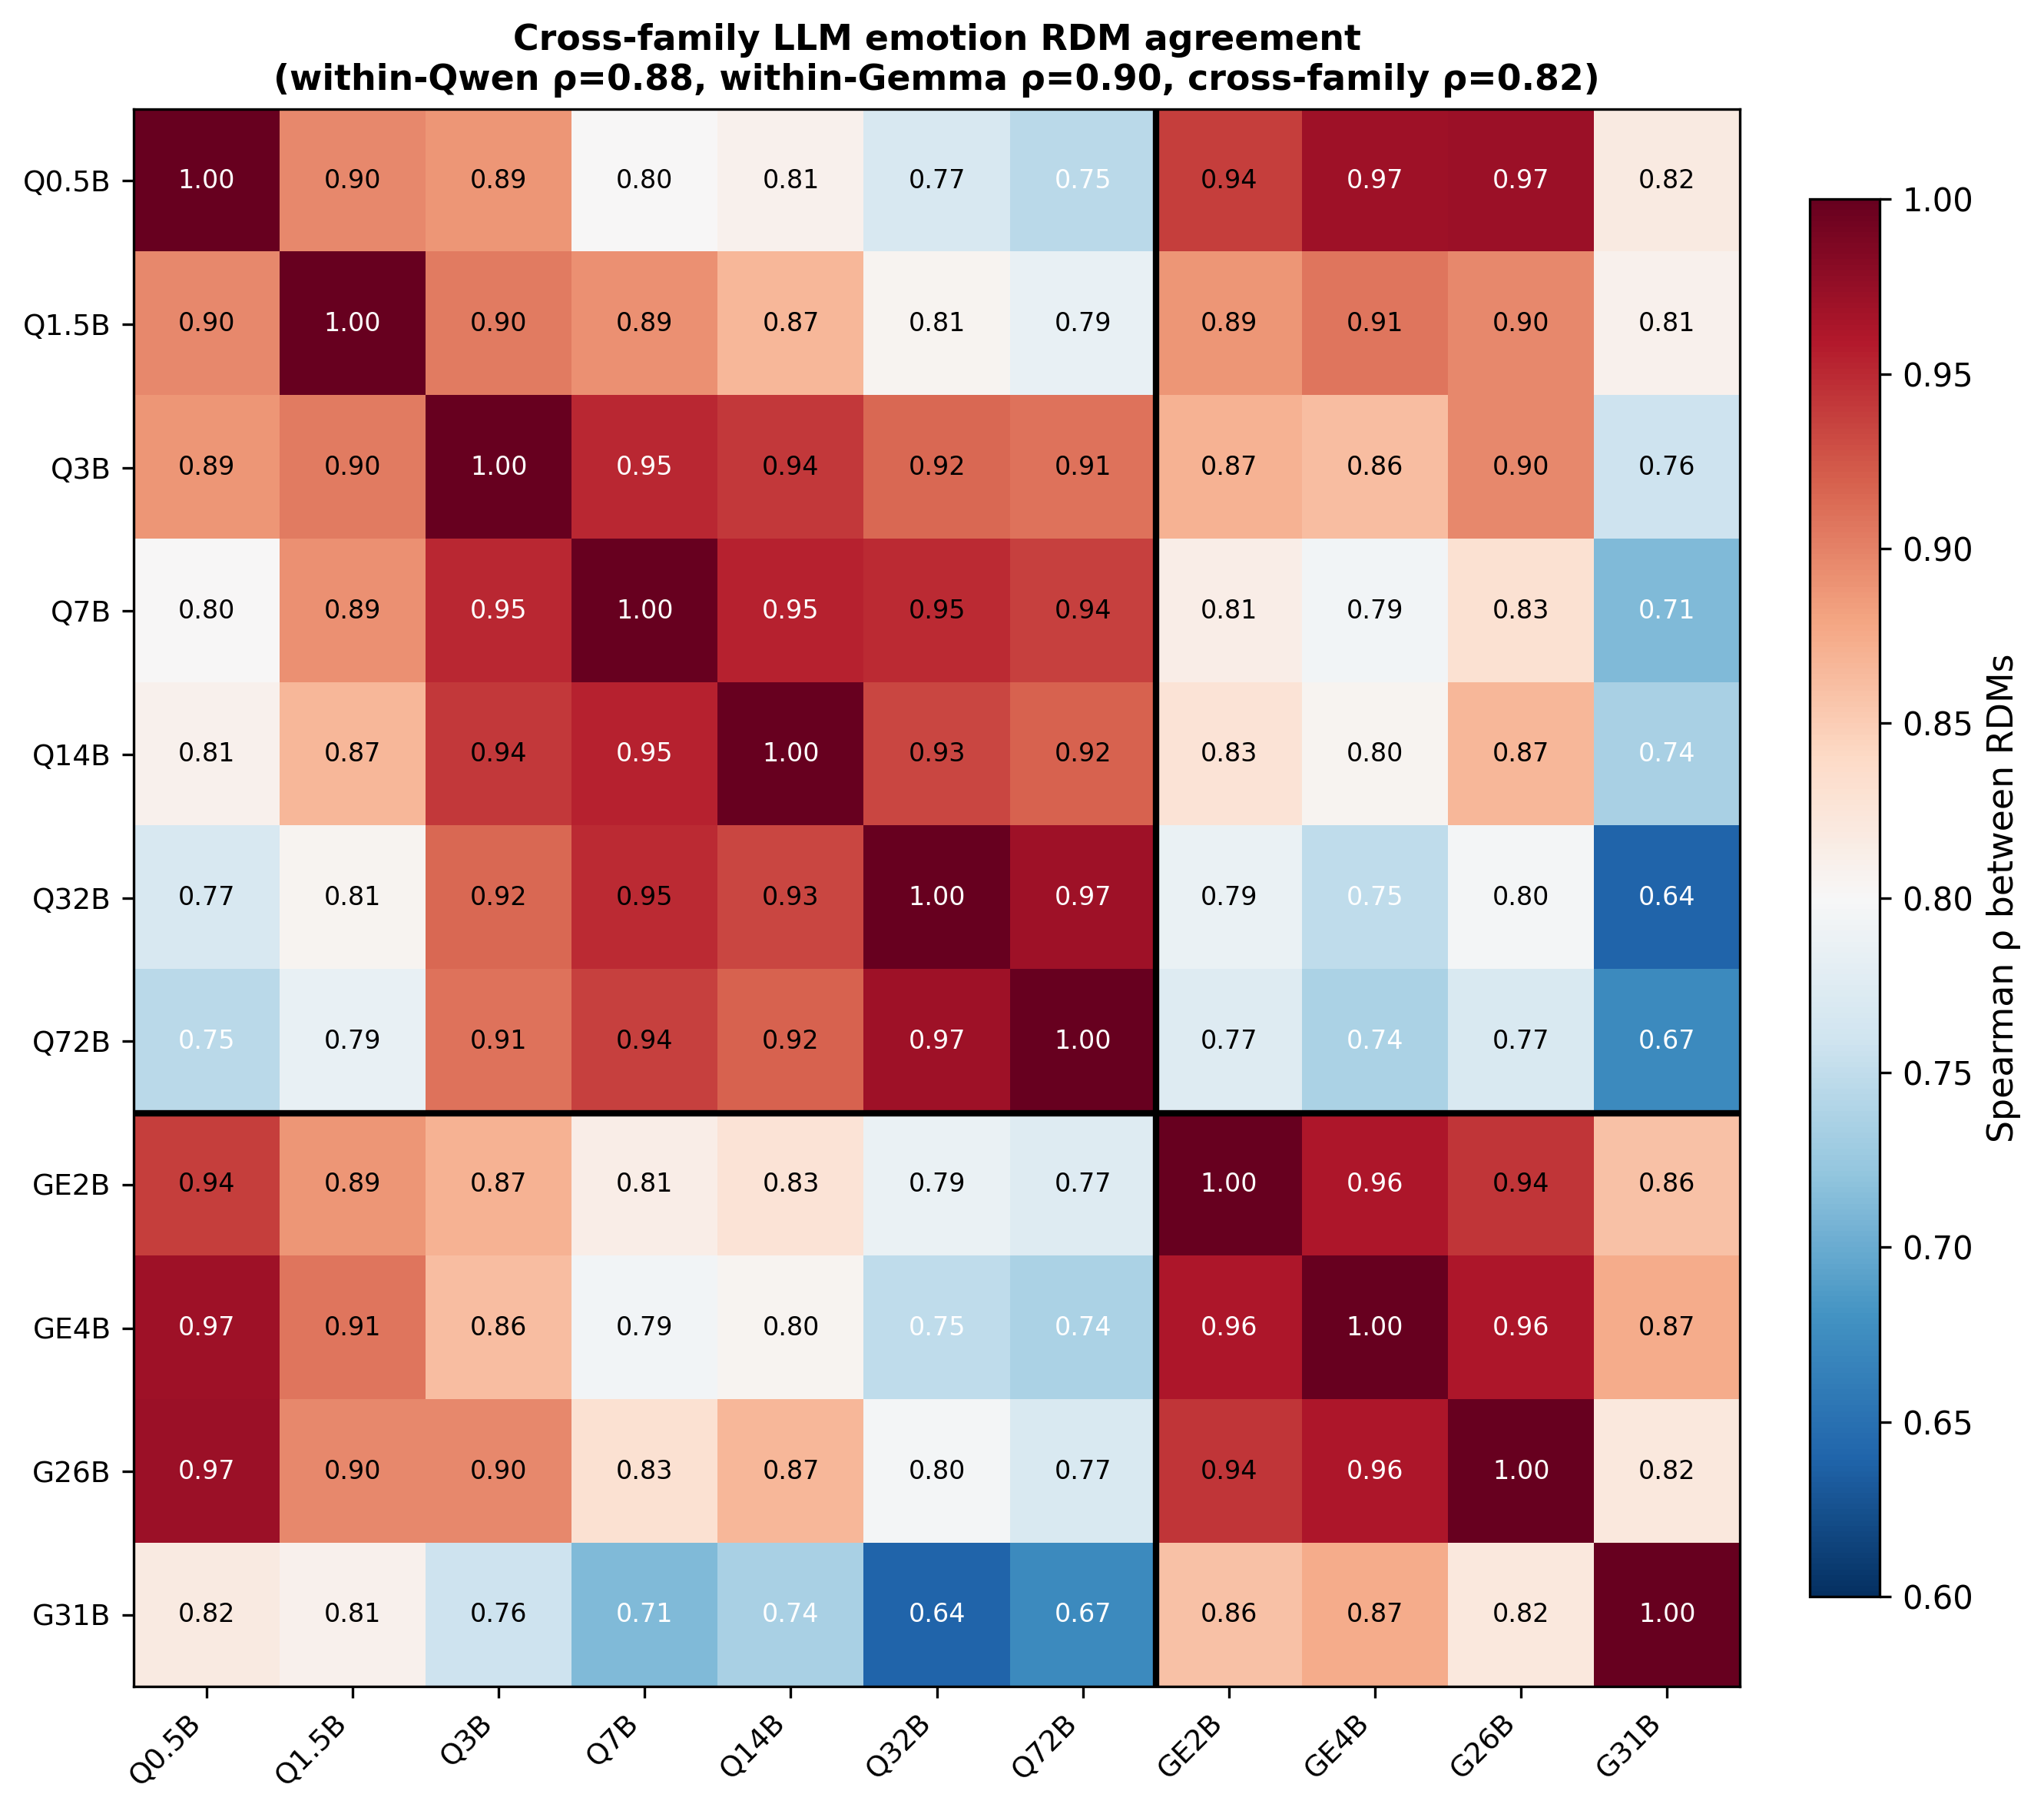
\includegraphics[width=0.85\linewidth]{figs/fig_cross_family_rdm.png}
    \caption{Cross-family RDM agreement matrix (Spearman $\rho$ between pairwise emotion-vector RDMs) for 11 instruction-tuned LLMs (7 Qwen sizes + 4 Gemma-4 variants). Within-family agreement (Qwen $\rho = 0.88$, Gemma $\rho = 0.90$) is only marginally higher than cross-family agreement ($\rho = 0.82$), confirming a universal LLM emotion geometry. Strongest cross-family pair: Qwen-0.5B $\leftrightarrow$ Gemma-4 26B-A4B at $\rho = 0.97$.}
    \label{fig:cross_family_rdm}
\end{figure}

We extend the LLM analysis to 11 instruction-tuned models from two families: 7 Qwen2.5 sizes (0.5B--72B) and 4 Gemma-4 variants (E2B, E4B, 26B-A4B, 31B). For each, we extract emotion vectors at the 67th-percentile layer and analyze (i) PC1--valence Pearson correlation, (ii) cluster separation, and (iii) representational dissimilarity matrices.

\begin{figure*}
\vspace{-4mm}
\centering
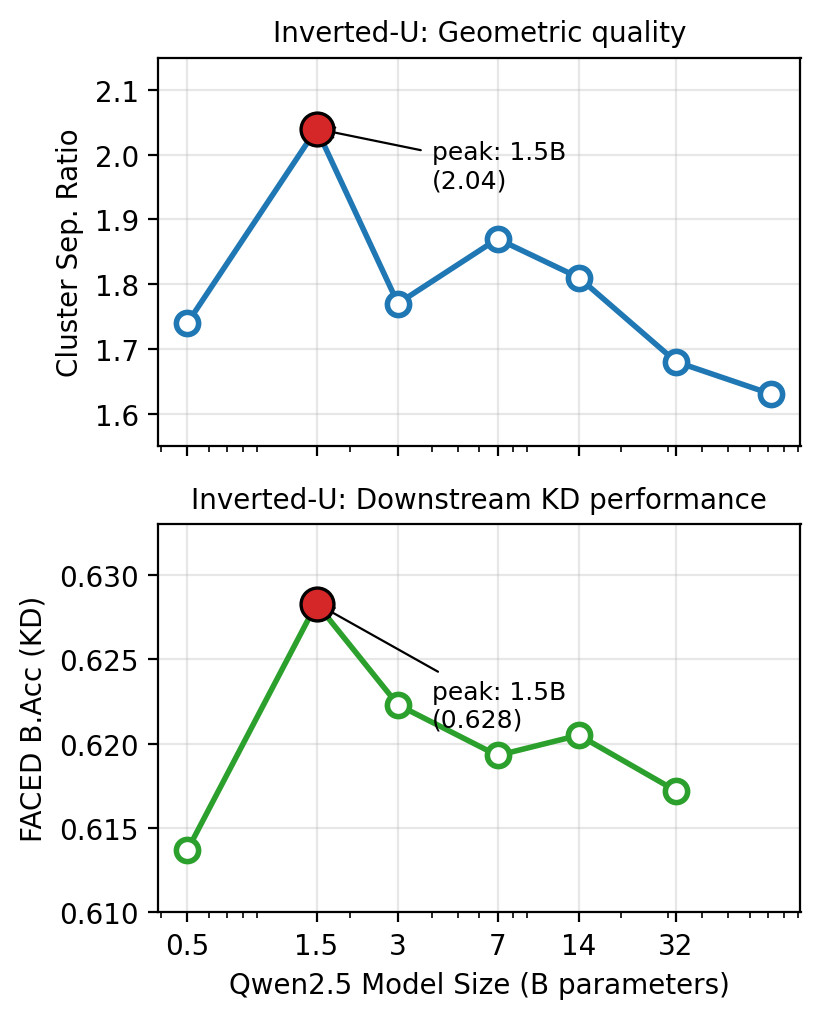
\includegraphics[width=0.5\linewidth]{figs/fig_inverted_u.png}
\caption{Two inverted-U curves with peak at Qwen-1.5B. \textbf{Top:} cluster separation ratio (geometric quality of emotion vectors). \textbf{Bottom:} downstream FACED balanced accuracy when used as KD teacher (mid-layer extraction). Both metrics agree that Qwen-1.5B is the optimal teacher size.}
\label{fig:inverted_u}
\end{figure*}

\noindent\textbf{Scale dependence.} \cref{fig:llm_scale_dual} shows the relationship between model size and emotion vector quality. For Qwen, valence correlation is high across all sizes ($r$ from $0.93$ at 0.5B to $0.98$ at 3B), while cluster separation peaks at 1.5B ($2.04$). The two metrics diverge because larger hidden dimensions ($896 \to 8192$) preserve the valence direction (high $r$) while shrinking inter-class distances relative to the ambient space. \cref{fig:inverted_u} (top) plots this inverted-U directly. Gemma-4 follows a similar pattern, with its 31B variant achieving $r = 0.972$. Critically, the inverted-U is mirrored in downstream EEG performance: when each Qwen size is used as a mid-layer KD teacher (\cref{fig:inverted_u}, bottom; full data in \cref{tab:supp_midlayer}), FACED balanced accuracy peaks at $\mathbf{0.628}$ for Qwen-1.5B and declines for both smaller and larger models. For KD, cluster separation is the operationally relevant metric, motivating our choice of small instruction-tuned LLMs as teachers.

\noindent\textbf{Cross-family universality.} To directly test whether the teacher's LLM family affects downstream EEG accuracy, we trained the full \ours\ pipeline with Gemma-27B as teacher instead of Qwen-0.5B. The result: $0.625 \pm 0.002$ vs.\ $0.622 \pm 0.005$ ($p = 0.38$, n.s.)---statistically identical, confirming that the emotion geometry is interchangeable across LLM families. \cref{fig:cross_family_rdm} shows pairwise RSA between RDMs of all 11 models. Within-Qwen agreement averages $\rho = 0.883 \pm 0.067$, within-Gemma $\rho = 0.904 \pm 0.055$, and Qwen$\leftrightarrow$Gemma cross-family $\rho = 0.818 \pm 0.081$. The cross-family agreement is only $\sim$$7\%$ lower than within-family, providing strong empirical support for the claim that LLM emotion geometry is universal across instruction-tuned models. The strongest cross-family pair (Qwen-0.5B$\leftrightarrow$Gemma-4 26B-A4B at $\rho = 0.97$) involves models that differ in family, size, and architecture (dense vs MoE) yet share nearly identical emotion structure. We also confirmed via linear probing that all 11 models achieve $100\%$ binary cluster purity for positive vs negative emotions at appropriate depth (\cref{sec:supp_llm}).

\noindent\textbf{Instruction tuning is critical.} To test whether the universality is driven by instruction tuning or by scale alone, we extracted emotion vectors from three base (non-instruction-tuned) language models: Pythia-1.4B, Bloom-560M, and TinyLlama-1.1B. All three produce vectors with \emph{no} valence structure (PC1--valence Pearson $r \in \{+0.30, 0.00, +0.27\}$, all $p > 0.4$), in contrast to every Qwen and Gemma instruction-tuned model ($|r| > 0.88$, $p < 10^{-3}$). This is consistent with the observation that instruction tuning steers LLMs toward explicit concept representations~\cite{scaling_brain_alignment2024}; the emotion geometry we distill is not a generic byproduct of language modeling but emerges from alignment training.

\noindent\textbf{Emotion-specific supervised fine-tuning degrades vector quality.} Motivated by the hypothesis that explicit emotion training would sharpen the teacher, we fine-tuned Qwen2.5-0.5B-Instruct on emotion-classification instructions (189- and 1898-instruction sets) and re-extracted vectors. Both SFT variants \emph{reduce} cluster separation monotonically with more instructions (from $1.74$ baseline to $1.70$ after 189 instructions, $-2.5\%$, and $1.63$ after 1898 instructions, $-6.6\%$), while the RDM geometry remains almost identical ($\rho > 0.99$). We interpret this as SFT compressing the rich relational structure into a tighter categorical decision boundary: useful for classification, but less informative as a KD teacher. We therefore retain the base instruction-tuned vectors throughout.

\subsection{Teacher Geometry: Fixed-Prototype Regularization}
\label{sec:fixed_prototype}
\vspace{-1mm}

\begin{figure}[!t]
    \centering
    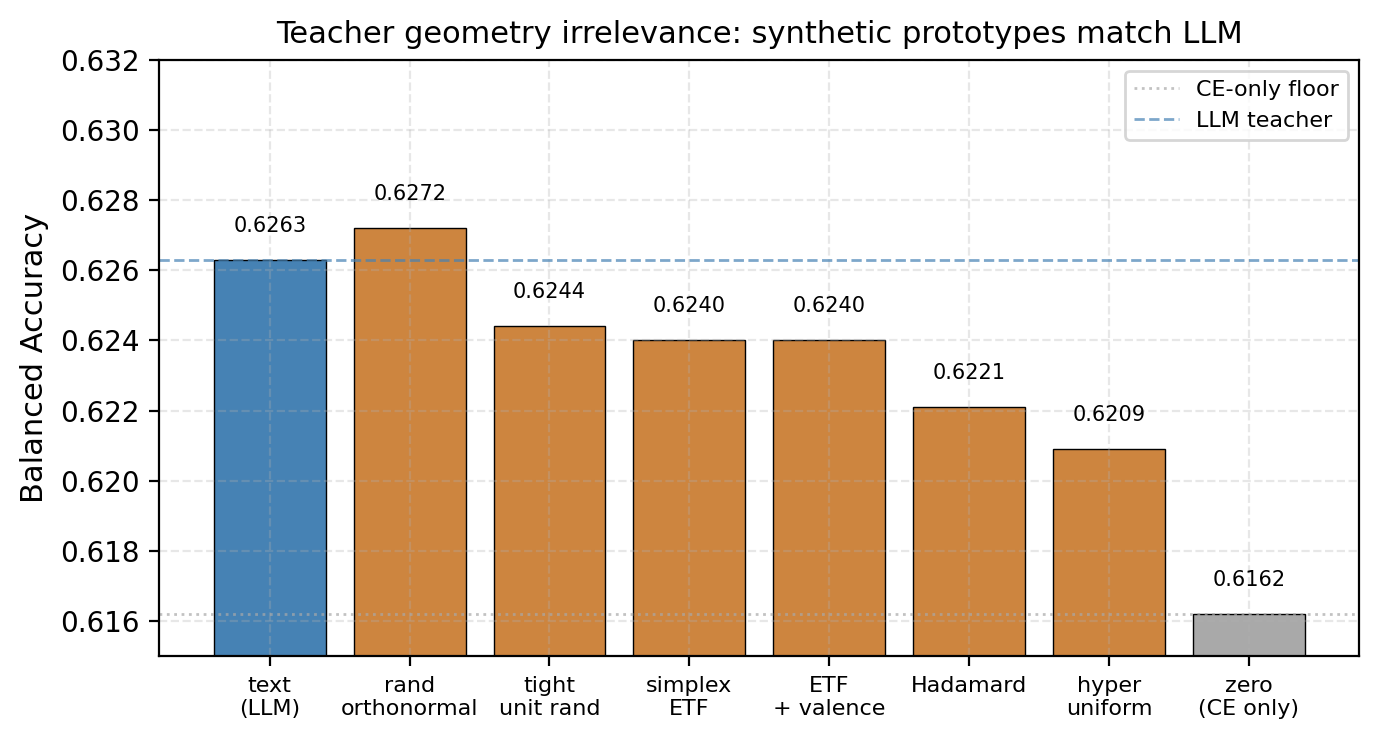
\includegraphics[width=0.88\linewidth]{figs/fig_synth_teachers.png}
    \caption{Synthetic-prototype KD on FACED (3 seeds per variant). A random orthonormal basis ($\mathbf{0.627}$) matches the LLM text teacher ($0.626$) within noise, while zero-teacher (no KD) falls to $0.616$. The full range across 7 synthetic variants spans just $0.006$, indicating that the KD framework functions as \emph{fixed-prototype regularization} rather than a mechanism for transferring LLM-specific knowledge.}
    \label{fig:synth_teachers}
\end{figure}

A natural follow-up to the universality findings above is: how \emph{specific} to language models is the teacher signal? We answer this by replacing the LLM-extracted vectors with seven synthetic teachers constructed directly from geometric primitives (no language model involved): (i) a random orthonormal basis via QR decomposition of a Gaussian matrix; (ii) a Simplex Equiangular Tight Frame~\cite{papyan2020neural}, the Neural-Collapse-optimal prototype geometry; (iii) a Hadamard binary orthogonal basis; (iv) a Tammes-style hyperspherical maximum-min-angle arrangement; (v) an ETF rotated to align its principal axis with ground-truth valence; (vi) a unit-norm random Gaussian tight frame; and (vii) a zero teacher (CE only, KD loss disabled as a control).

\cref{fig:synth_teachers} shows that all seven synthetic variants yield downstream B.Acc within $[0.616, 0.627]$---a range of $0.011$, barely larger than the seed-level noise of the LLM teacher itself. The random orthonormal basis ($0.627$) actually slightly exceeds the LLM text teacher ($0.626$), and the Simplex ETF matches it at $0.624$. Only the zero-teacher control drops meaningfully to $0.616$, recovering the aug-only baseline. This result is strong evidence that \textbf{the operative mechanism of our KD term is fixed-prototype regularization}: the student head is pulled toward a consistent set of orthogonal targets, and the \emph{specific content} of the targets (LLM-extracted, ETF, or random) is largely irrelevant. Complementary evidence comes from a quality-spectrum sweep (\cref{sec:supp_qspec}): ten teacher variants spanning PC1--valence correlations from $0.19$ to $0.97$ produce downstream B.Acc within a span of $0.009$ and a Pearson correlation of $r = +0.23$ ($p = 0.52$, n.s.). Both experiments converge on the same conclusion: above a very low floor, teacher quality is not the binding constraint.

We emphasize that this does \emph{not} diminish the value of the LLM geometry as an \emph{interpretable} artifact---the PCA-recovered circumplex (\cref{fig:pca}) and cross-family universality (\cref{fig:cross_family_rdm}) remain meaningful analyses of how LLMs encode emotion. What the synthetic-prototype experiment changes is our understanding of how the KD \emph{training signal} works: it regularizes the projection head's output geometry toward a non-collapsed configuration, and any sufficiently structured set of orthogonal targets suffices.

\subsection{Representational Alignment via CKA}
\label{sec:cka}
\vspace{-1mm}

\begin{figure}[!t]
    \centering
    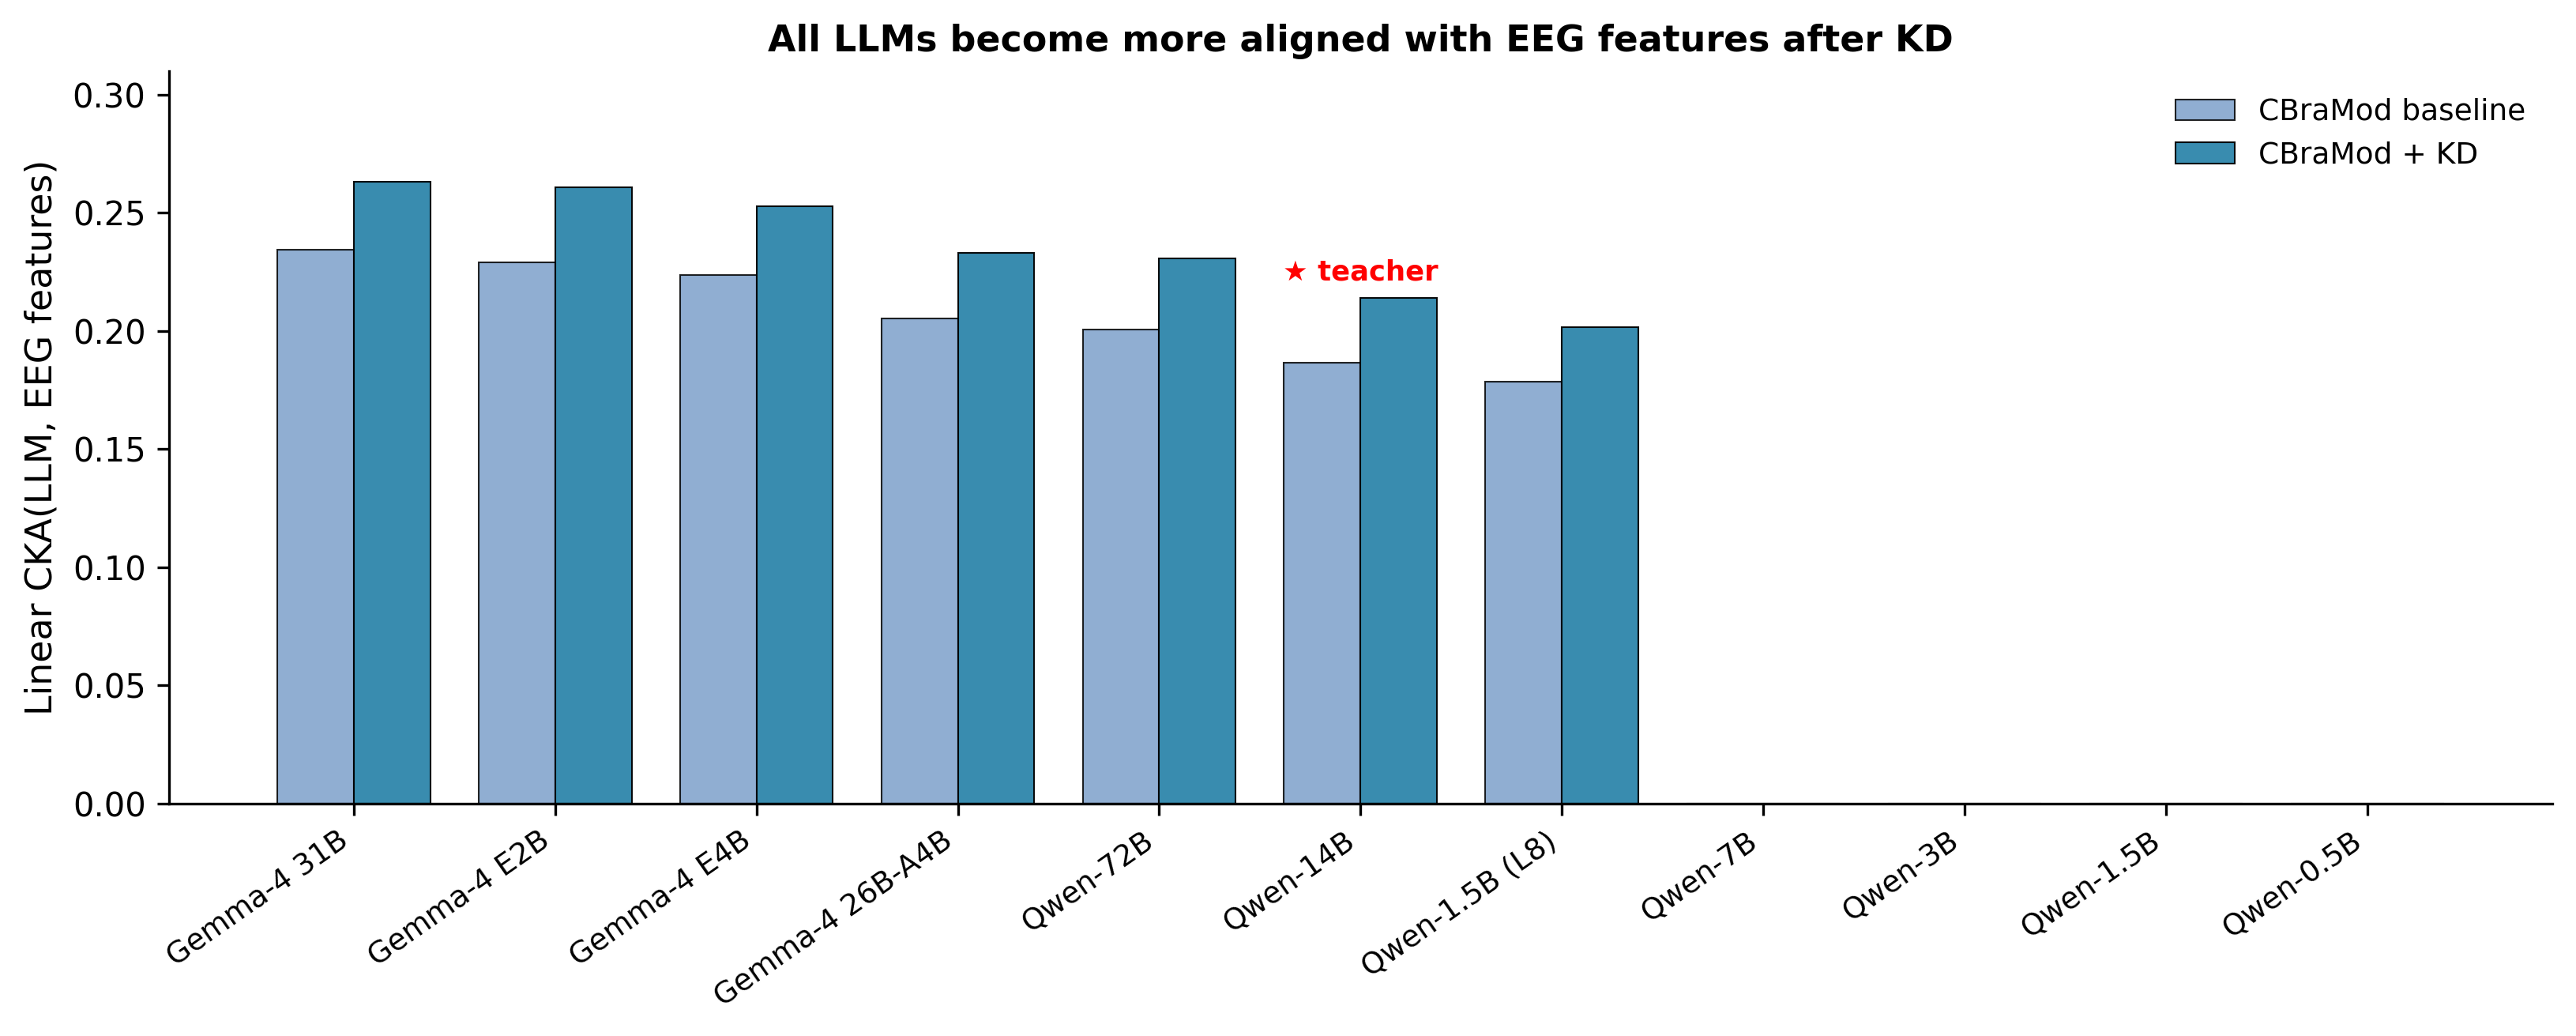
\includegraphics[width=0.96\linewidth]{figs/fig_cka_increase.png}
    \caption{Linear CKA between LLM per-sample features and CBraMod EEG penultimate features, baseline vs +KD. \emph{All LLMs become more aligned with EEG features after KD} ($\Delta$CKA $\approx +0.03$ across the board). The teacher used for training (Qwen2.5-0.5B, marked $\star$) is \emph{not} the most-aligned LLM after distillation: Gemma-4 31B has the highest CKA, indicating that KD absorbs a universal emotion structure rather than overfitting to one specific teacher.}
    \label{fig:cka_increase}
\end{figure}

To directly test whether KD makes the EEG model's representations more brain-LLM aligned, we compute Linear Centered Kernel Alignment (CKA)~\cite{kornblith2019cka}, the standard metric for measuring representational similarity in NeurIPS-era brain-LLM alignment work~\cite{rethinking_cka_kd2024,brain_llm_compression2023}. For each test sample, we use the LLM emotion vector for that sample's class as a per-sample feature, and we compare these against CBraMod's penultimate features (200-dim) before and after KD on $1{,}932$ FACED test samples.

\cref{fig:cka_increase} shows a uniform pattern: LLMs in our suite---including those from a different family from the training teacher---become \emph{more} CKA-aligned with CBraMod's features after KD, with $\Delta$CKA $\approx +0.03$ across the board. Notably, the highest post-KD alignment is achieved with Gemma-4 31B (CKA $= 0.263$), even though training used Qwen2.5-0.5B as the teacher. This argues that KD does not simply pull EEG features toward the specific teacher; it absorbs a universal emotion structure that aligns with all sufficiently capable instruction-tuned LLMs. We find a similar pattern for kernel CKA (RBF) and for class-mean RSA, with Linear CKA showing the cleanest signal.

\subsection{Layerwise Valence/Arousal Probing}
\label{sec:layerwise_probe}
\vspace{-1mm}

\begin{figure}[!t]
    \centering
    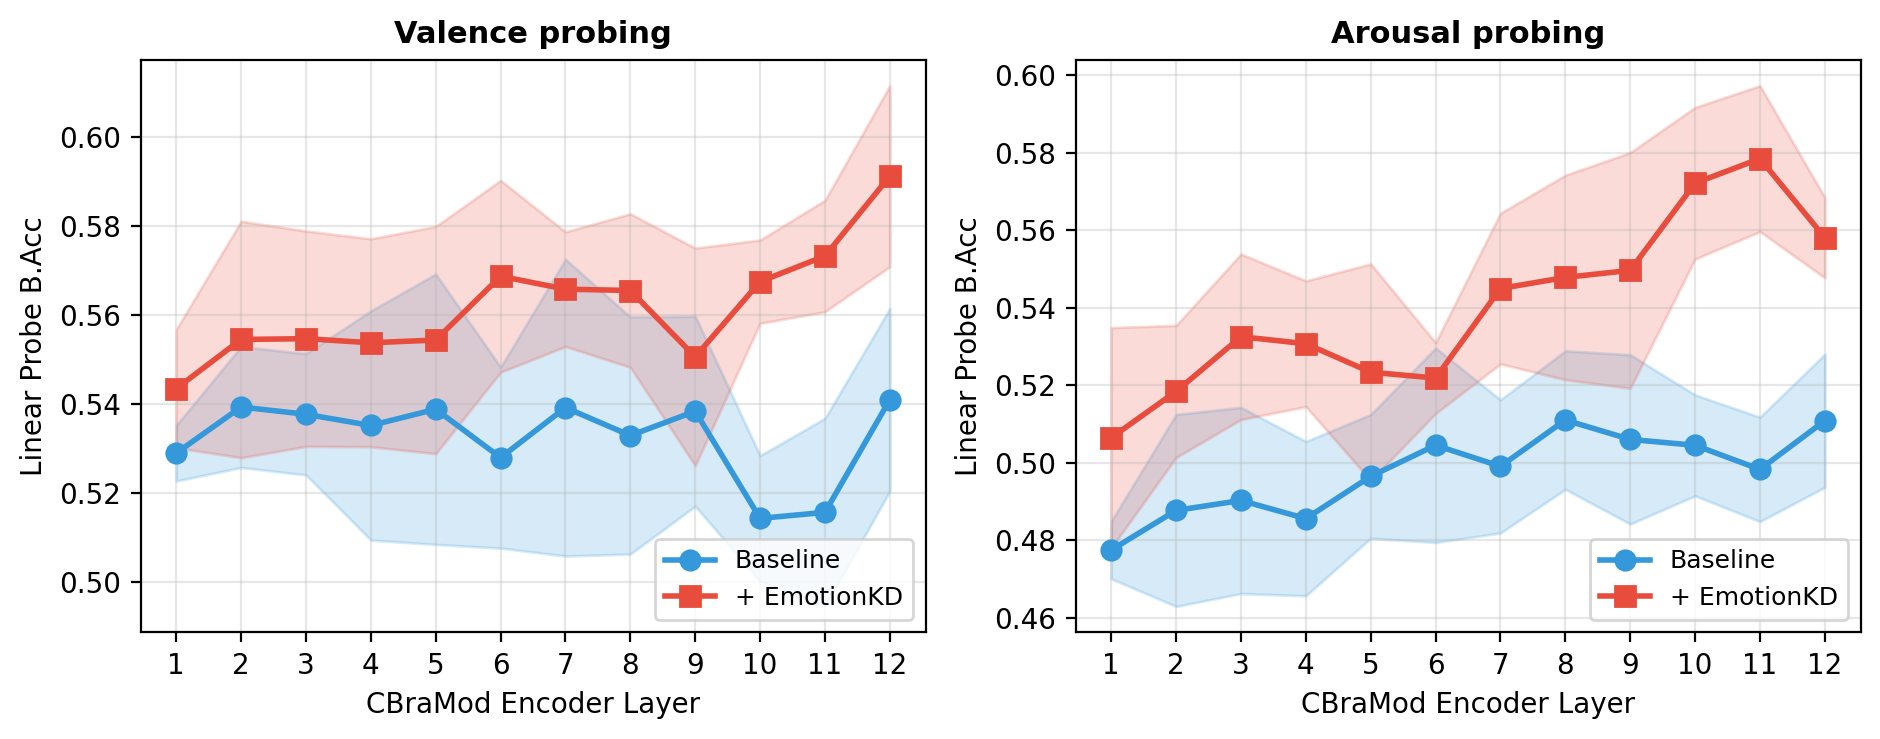
\includegraphics[width=0.92\linewidth]{figs/fig_layerwise_probe.png}
    \caption{Linear probing of all 12 CBraMod encoder layers for valence (left; positive vs.\ negative, excluding neutral) and arousal (right; high vs.\ low). Lines show 5-fold balanced accuracy with $\pm 1$ std shaded. KD improves probe accuracy at \emph{every} layer, with the strongest effect at deeper layers (up to $+5.7\%$ for valence at layer 10 and $+8.0\%$ for arousal at layer 10). The effect is consistent with prior LLM interpretability findings~\cite{tak2025emotion_interpretability,decoding_emotion_deep2024}, showing that KD pushes emotion-dimension information into the late encoder layers where it supports downstream classification.}
    \label{fig:layerwise_probe}
\end{figure}

To mechanistically test whether KD shapes the internal EEG representations along the valence--arousal axes, we train linear probes on each of CBraMod's 12 encoder layers for (i) binary valence (positive vs.\ negative, excluding neutral), and (ii) binary arousal (high vs.\ low, following the standard circumplex mapping~\cite{russell1980circumplex}: amusement/joy/anger/fear/disgust are high-arousal; inspiration/tenderness/sadness/neutral are low). Probes are $L_2$-regularized logistic regression with 5-fold stratified cross-validation.

\cref{fig:layerwise_probe} shows the result. KD strictly dominates baseline at every layer for both tasks, and the gap widens toward deeper layers. At layer 10, KD-trained features reach $0.573$ valence B.Acc and $0.579$ arousal B.Acc, compared to $0.516$ and $0.498$ for baseline---an increase of $+5.7\%$ and $+8.0\%$, respectively. This provides direct mechanistic evidence that LLM-guided supervision \emph{rearranges} the EEG encoder's internal geometry to concentrate valence and arousal information in the late layers that feed the classifier, mirroring the depth-dependent emotion-encoding pattern reported in LLMs~\cite{tak2025emotion_interpretability,decoding_emotion_deep2024}.

\subsection{Representational Visualization (t-SNE)}
\label{sec:tsne}
\vspace{-1mm}

\begin{figure}[!t]
    \centering
    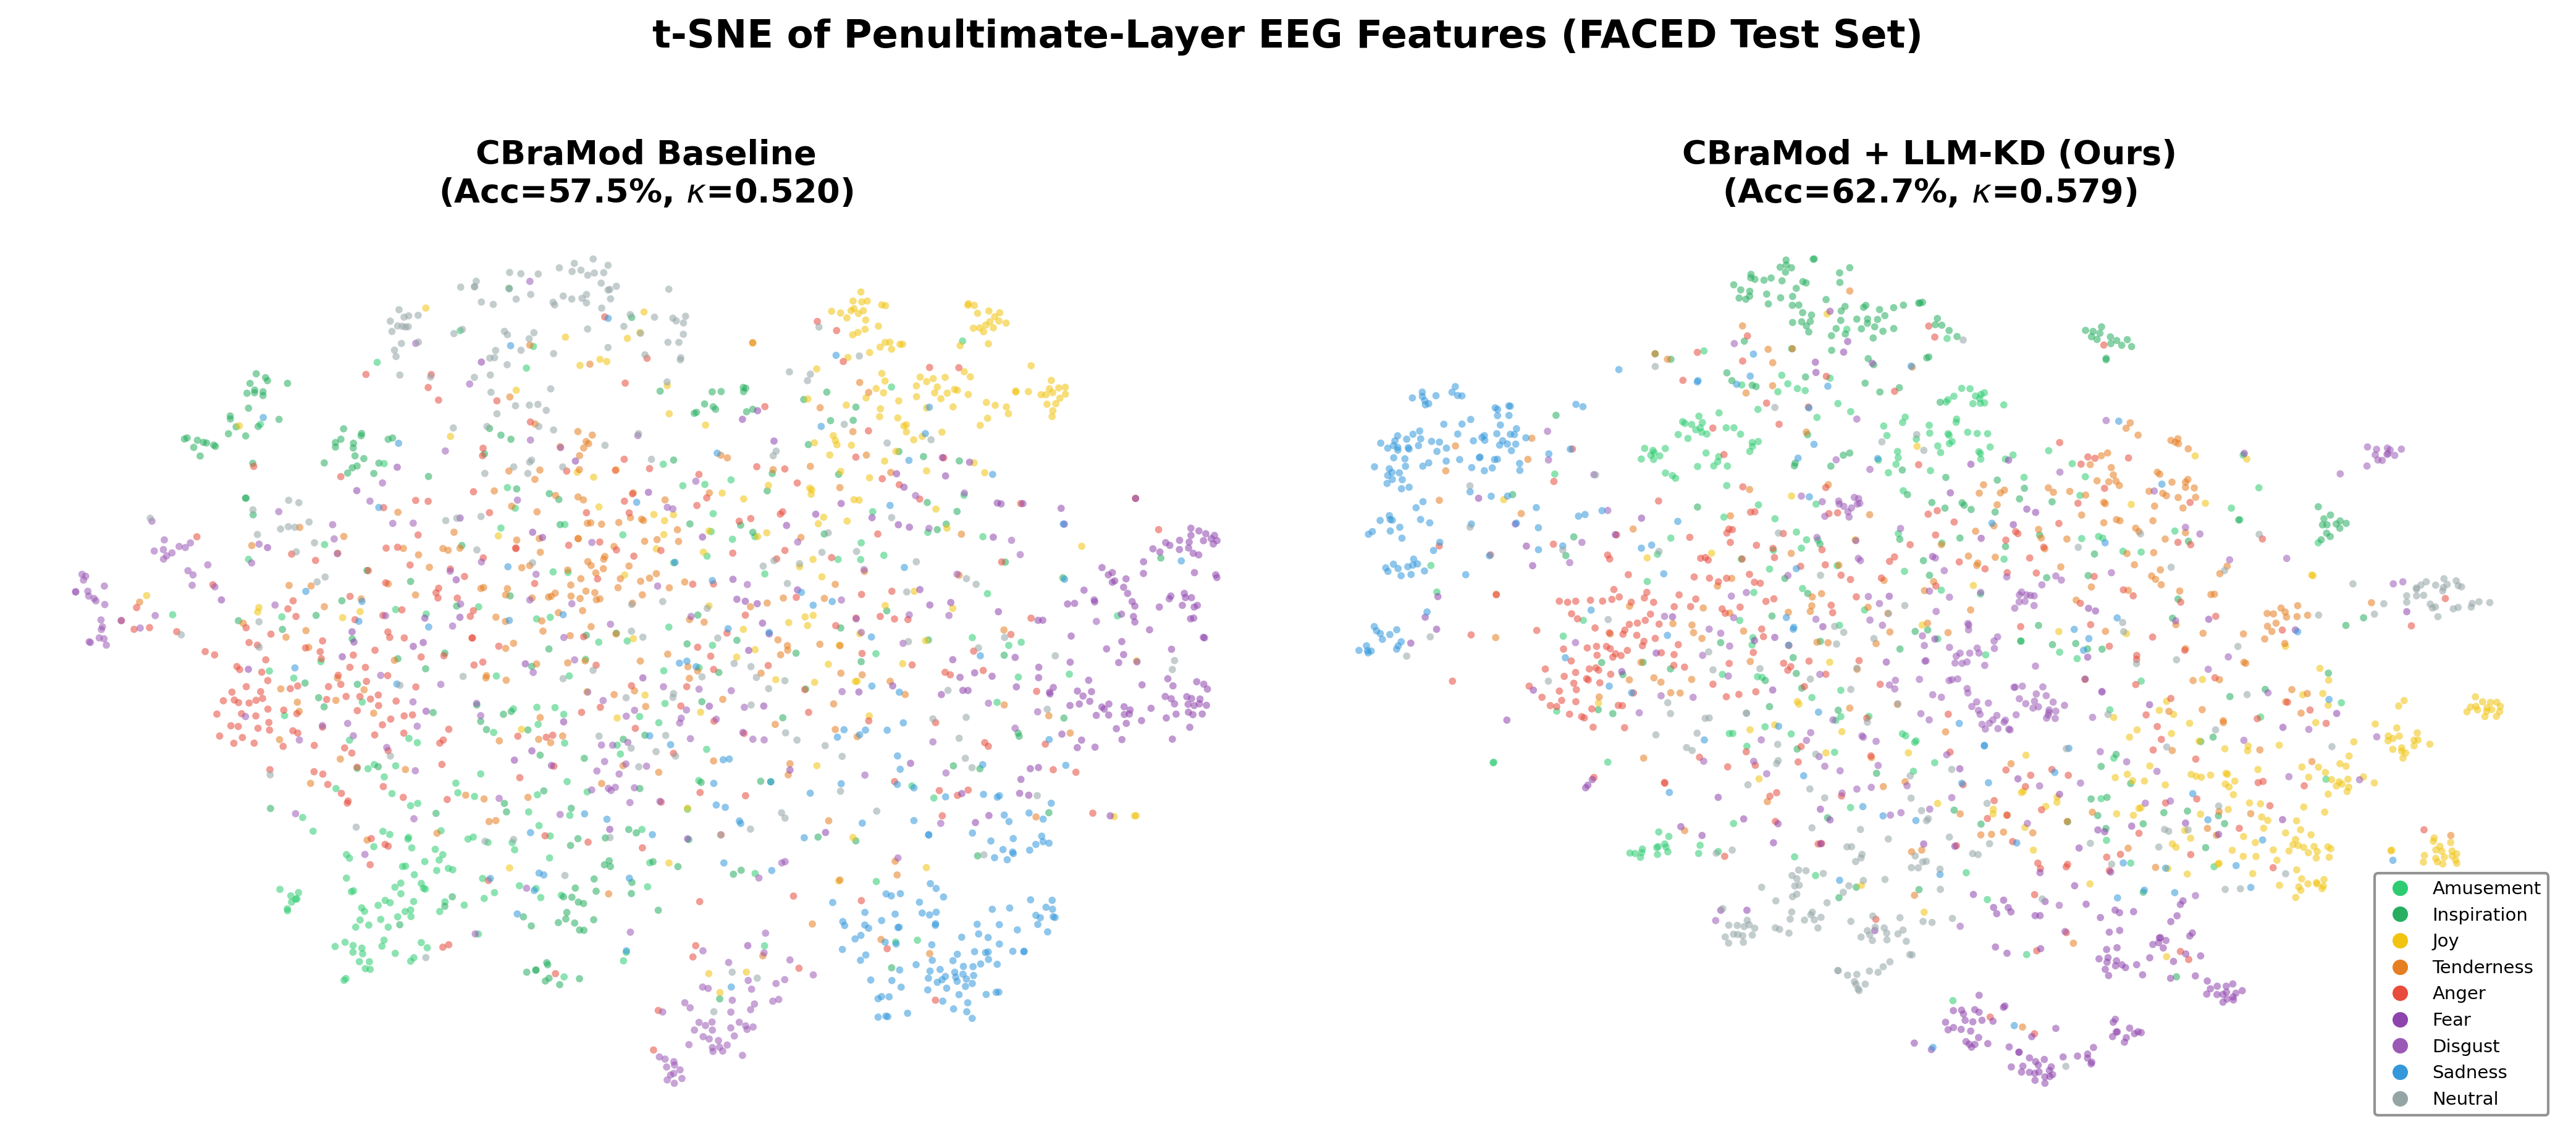
\includegraphics[width=0.9\linewidth]{figs/fig_tsne_comparison.png}
    \caption{t-SNE visualization of learned EEG representations on the FACED test set. \textbf{Left:} CBraMod baseline (B.Acc 57.5\%, $\kappa = 0.520$). \textbf{Right:} CBraMod $+$ \ours\ (B.Acc 62.7\%, $\kappa = 0.579$). Emotion clusters become more distinct after KD-guided training.}
    \label{fig:tsne}
\end{figure}

\cref{fig:tsne} shows t-SNE projections of CBraMod features on FACED before and after \ours. Emotion clusters become more discrete after KD. Extended three-panel visualizations including the adapter64 variant are presented in \cref{fig:cluster_tsne_3panel,fig:cluster_umap_3panel}, with convex hull overlays in \cref{fig:cluster_convex_hull} further quantifying the reduced inter-class overlap.

\subsection{KD Isolation: Augmentation is Required}
\label{sec:kd_isolation}
\vspace{-1mm}

\begin{table}[!t]
\caption{KD isolation on FACED. Without augmentation, KD and adapters \emph{hurt} performance ($-0.5\%$ to $-1.3\%$). KD only helps \emph{on top of} augmentation, acting as a complementary regularizer.}
\small
\centering
\begin{tabular}{lcccc}
\toprule
Config & Aug? & B.Acc & $\Delta$ \\
\midrule
\multicolumn{4}{l}{\textit{Without augmentation:}} \\
Baseline & \xmark & 0.572 & --- \\
+ KD (3L-BN proj) & \xmark & 0.559 & $-1.3\%$ \\
+ Adapter64 + KD & \xmark & 0.567 & $-0.5\%$ \\
\midrule
\multicolumn{4}{l}{\textit{With augmentation ($p_{\text{aug}} = 0.6$):}} \\
Aug only & \cmark & 0.616 & $+4.4\%$ \\
+ KD (3L-BN proj) & \cmark & 0.622 & $+5.0\%$ \\
+ Adapter64 + InfoNCE & \cmark & 0.620 & $+4.8\%$ \\
\rowcolor{blond}
\textbf{+ Adapter64 + KD} & \cmark & \textbf{0.628} & $\mathbf{+5.6\%}$ \\
\bottomrule
\end{tabular}
\label{tab:kd_isolation}
\end{table}

A natural question is whether KD provides value independently of augmentation, or only in combination. \cref{tab:kd_isolation} presents the full factorial: we train both KD and adapter64 configurations with and without augmentation ($p_{\text{aug}} = 0$ vs.\ $0.6$). The result is striking: \textbf{without augmentation, KD actively hurts} ($-1.3\%$ for full fine-tuning, $-0.5\%$ for adapter64). The 3-layer BN projection head adds model capacity that, without the regularization provided by temporal jitter and other augmentations, leads to mild overfitting. With augmentation, the same KD signal adds $+0.6\%$ on top of aug-only ($0.622$ vs.\ $0.616$), and adapter64 further improves to $0.628$.

This pattern---where KD helps only in combination with augmentation---reveals that the two mechanisms are \emph{complementary regularizers}: augmentation regularizes the \emph{input} space (forcing timing-invariant features), while KD regularizes the \emph{output} space (providing graded soft targets that encode inter-class relationships). Neither alone matches their combination. The finding is even stronger in the cross-subject LOSO setting: KD without augmentation \emph{significantly} hurts performance ($-2.2\%$, $p = 0.029$, all 5 folds negative), while KD with augmentation significantly helps ($+2.4\%$, $p = 0.0002$). This confirms that the complementary-regularizer mechanism is not an artifact of the within-subject protocol.

\noindent\textbf{Why does KD require augmentation?} We propose the following mechanistic explanation, supported by three lines of evidence. Without augmentation, the model memorizes the fixed training set rapidly (training accuracy reaches $\sim$0.95 by epoch 10), at which point CE gradients are near-zero and KD becomes the dominant gradient signal. But KD pushes predictions toward \emph{soft} distributions---teaching that anger should look somewhat like disgust---which actively interferes with the hard-label classifications the model has already memorized. The 3-layer BN projection head (0.83M parameters) exacerbates this by overfitting to the training data; indeed, an older 2-layer projection without BN yielded KD-only $\approx$ baseline ($0.571$ vs.\ $0.572$) rather than \emph{worse}, confirming that the projection head's excess capacity is the source of degradation. With augmentation, the picture inverts: temporal jitter ($\pm$100\,ms shifts) ensures the model never fully ``solves'' the training set, CE gradients remain active throughout training, and KD provides a \emph{stable geometric anchor}---encoding that anger remains closer to disgust than to joy regardless of augmentation---that resolves the ambiguity augmentation creates. Four pieces of evidence support this account.

\begin{figure}[!t]
    \centering
    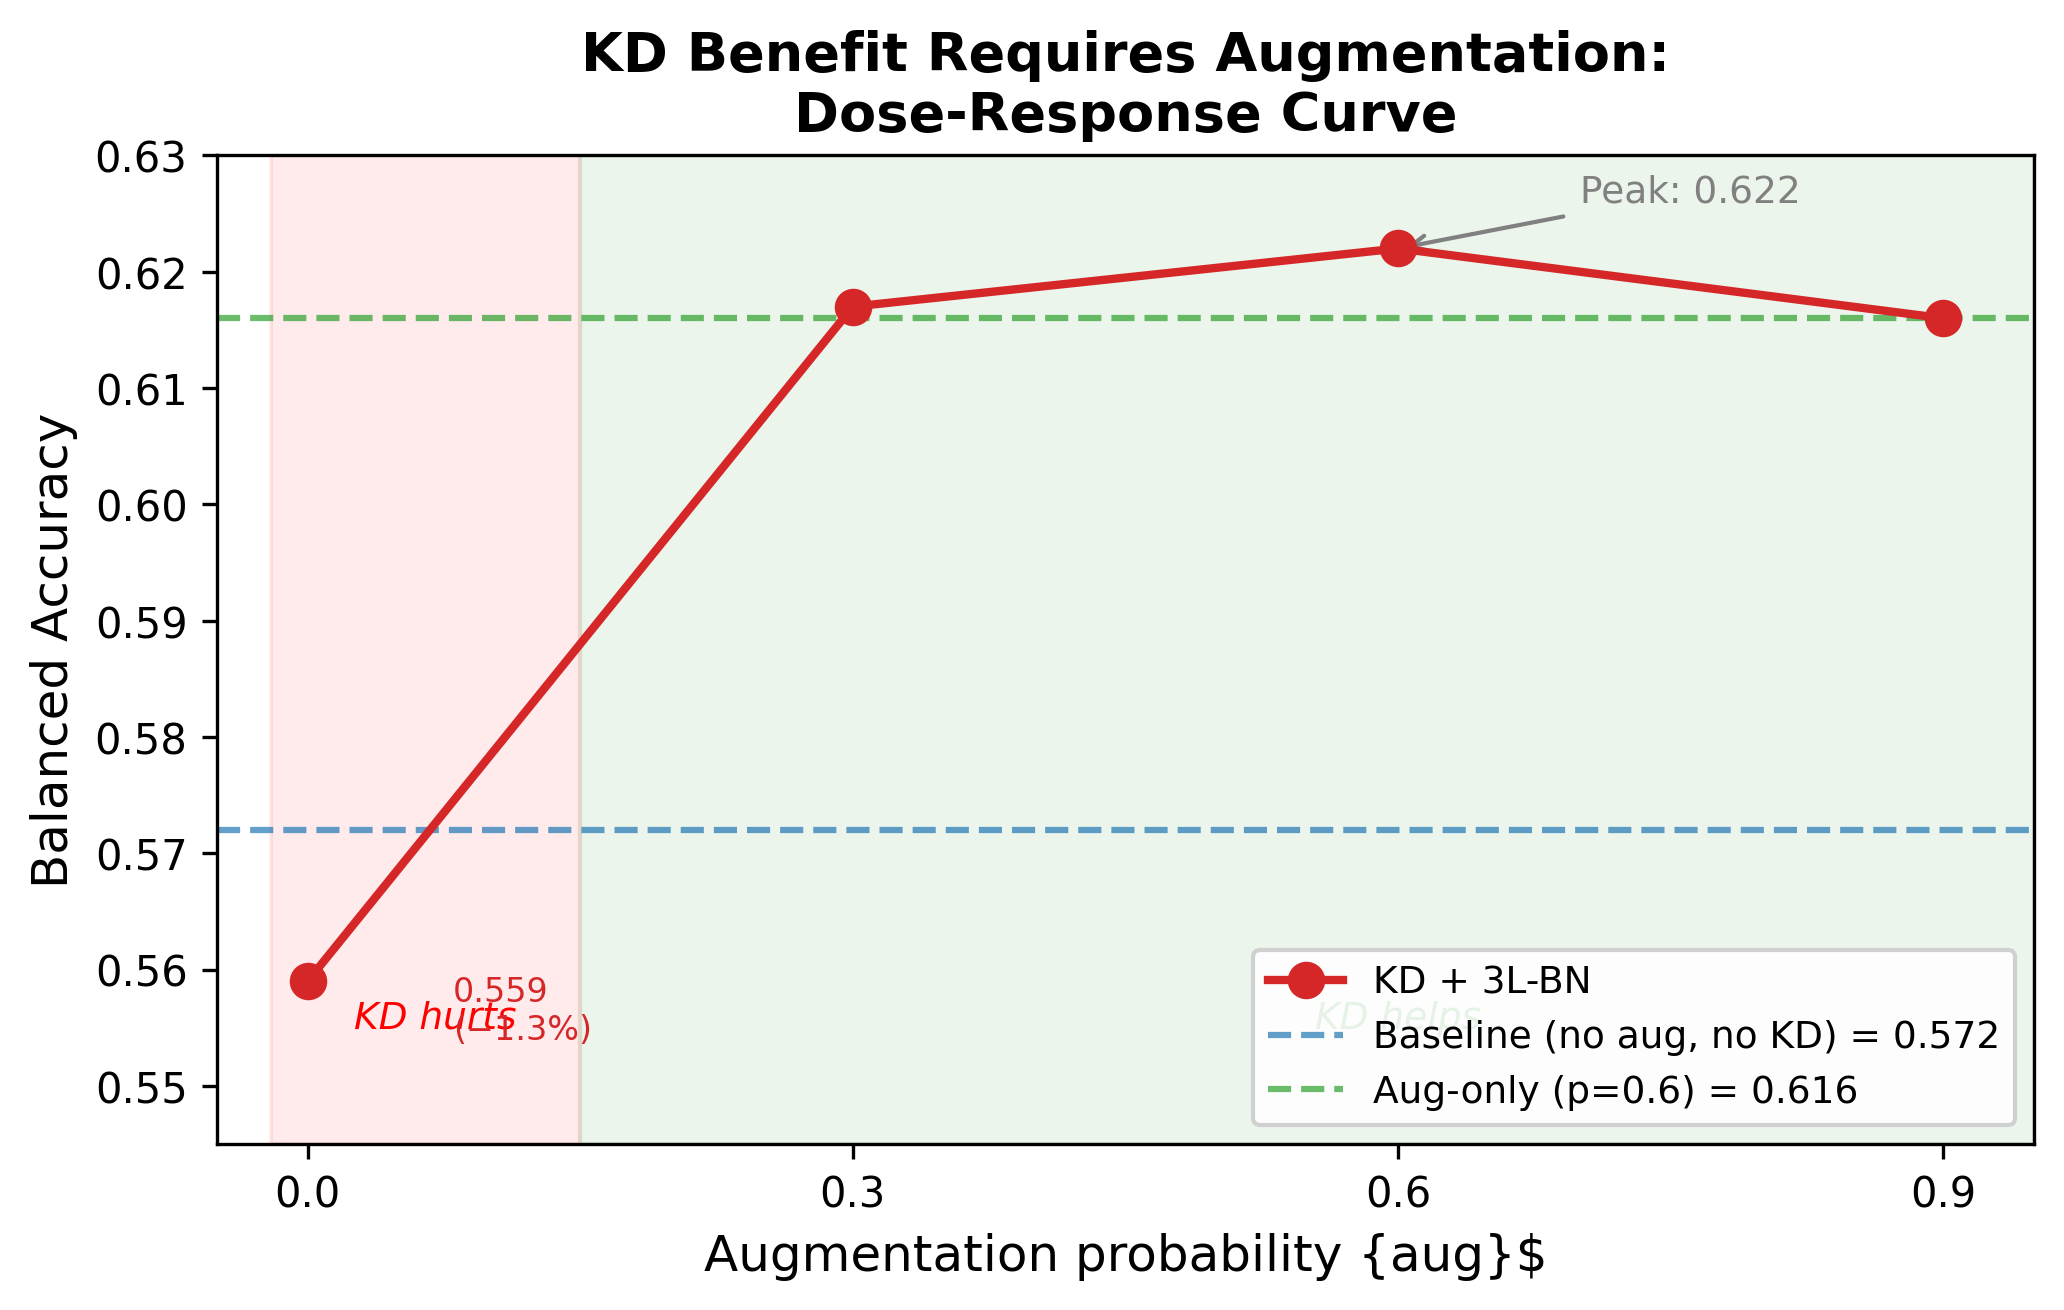
\includegraphics[width=\linewidth]{figs/fig_kd_dose_response.png}
    \caption{Dose-response: augmentation probability vs.\ KD accuracy on FACED. Without augmentation ($p = 0$), KD \emph{hurts} ($-1.3\%$). With increasing augmentation, KD benefit grows, peaking at $p = 0.6$ ($0.622$). Excessive augmentation ($p = 0.9$) slightly degrades due to input noise. The aug-only baseline (dashed green) shows that KD adds value only when augmentation is present.}
    \label{fig:kd_dose_response}
\end{figure}

\noindent(i)~\textbf{Dose-response curve} (\cref{fig:kd_dose_response}): sweeping $p_{\text{aug}} \in \{0, 0.3, 0.6, 0.9\}$ reveals that KD benefit grows monotonically with augmentation intensity up to $p = 0.6$, then slightly declines at $p = 0.9$ due to excessive input noise. At $p = 0$, KD is $-1.3\%$ \emph{below} baseline; at $p = 0.3$, KD recovers to $0.617$ (matching aug-only); at $p = 0.6$, KD reaches its peak at $0.622$ ($+0.6\%$ over aug-only).
(ii)~KD-only models select best checkpoints at mean epoch $22.8$ (same as baseline), while KD+aug models select at epoch $37.0$---augmentation extends the useful training horizon where KD's geometric signal adds value.
(iii)~The effect is stronger in LOSO ($-2.2\%$ without vs.\ $+2.4\%$ with aug), where cross-subject variability creates more ``uncertainty'' for KD to resolve.
(iv)~\textbf{Projection head capacity control}: training with the same 3L-BN architecture but $\lambda = 0$ (no KD loss) yields $0.614$---statistically identical to aug-only ($0.616$)---confirming that the projection head itself is neutral and only becomes beneficial when activated by the KD loss. Conversely, KD with a simpler 2-layer projection (no BN) yields $0.611$, showing that the 3L-BN architecture amplifies KD's benefit by $+1.1\%$.

\subsection{Mixup Augmentation}
\label{sec:mixup}
\vspace{-1mm}

Beyond the loss-level KD signal, we explore whether LLM emotion vectors can contribute at the \emph{data} level via mixup augmentation~\cite{zhang2018mixup}. Specifically, we bias mixup partner selection toward semantically similar emotions using the LLM cosine similarity matrix as a sampling prior: $P(y_b \mid y_a) \propto \exp(\cos(\mathbf{v}_{y_a}, \mathbf{v}_{y_b}) / \tau)$ with $\tau = 0.3$, inspired by C-Mixup~\cite{yao2022cmixup}.

\begin{table}[!t]
\caption{Mixup augmentation on FACED. LLM-guided mixup significantly improves over the KD baseline ($p = 0.003$, 10 seeds, Cohen's $d = 1.27$). However, the ablation reveals that random partner selection performs comparably ($p = 0.48$ for LLM vs Random), indicating the gain comes from mixup regularization rather than LLM-specific guidance.}
\small
\centering
\begin{tabular}{lccccc}
\toprule
Method & B.Acc & $n$ & $\Delta$ vs KD & $p$ vs KD \\
\midrule
KD baseline (kd\_full\_bn3) & 0.622 $\pm$ 0.005 & 10 & --- & --- \\
Random mixup ($\tau = 100$) & 0.625 $\pm$ 0.006 & 5 & $+$0.3\% & 0.074 \\
LLM-guided mixup ($\tau = 0.3$) & \textbf{0.630} $\pm$ 0.011 & 10 & $\mathbf{+0.8\%}$ & \textbf{0.009} \\
\midrule
LLM vs Random & --- & 5 & $+$0.5\% & 0.48 (n.s.) \\
\bottomrule
\end{tabular}
\label{tab:mixup}
\end{table}

\begin{figure}[!t]
    \centering
    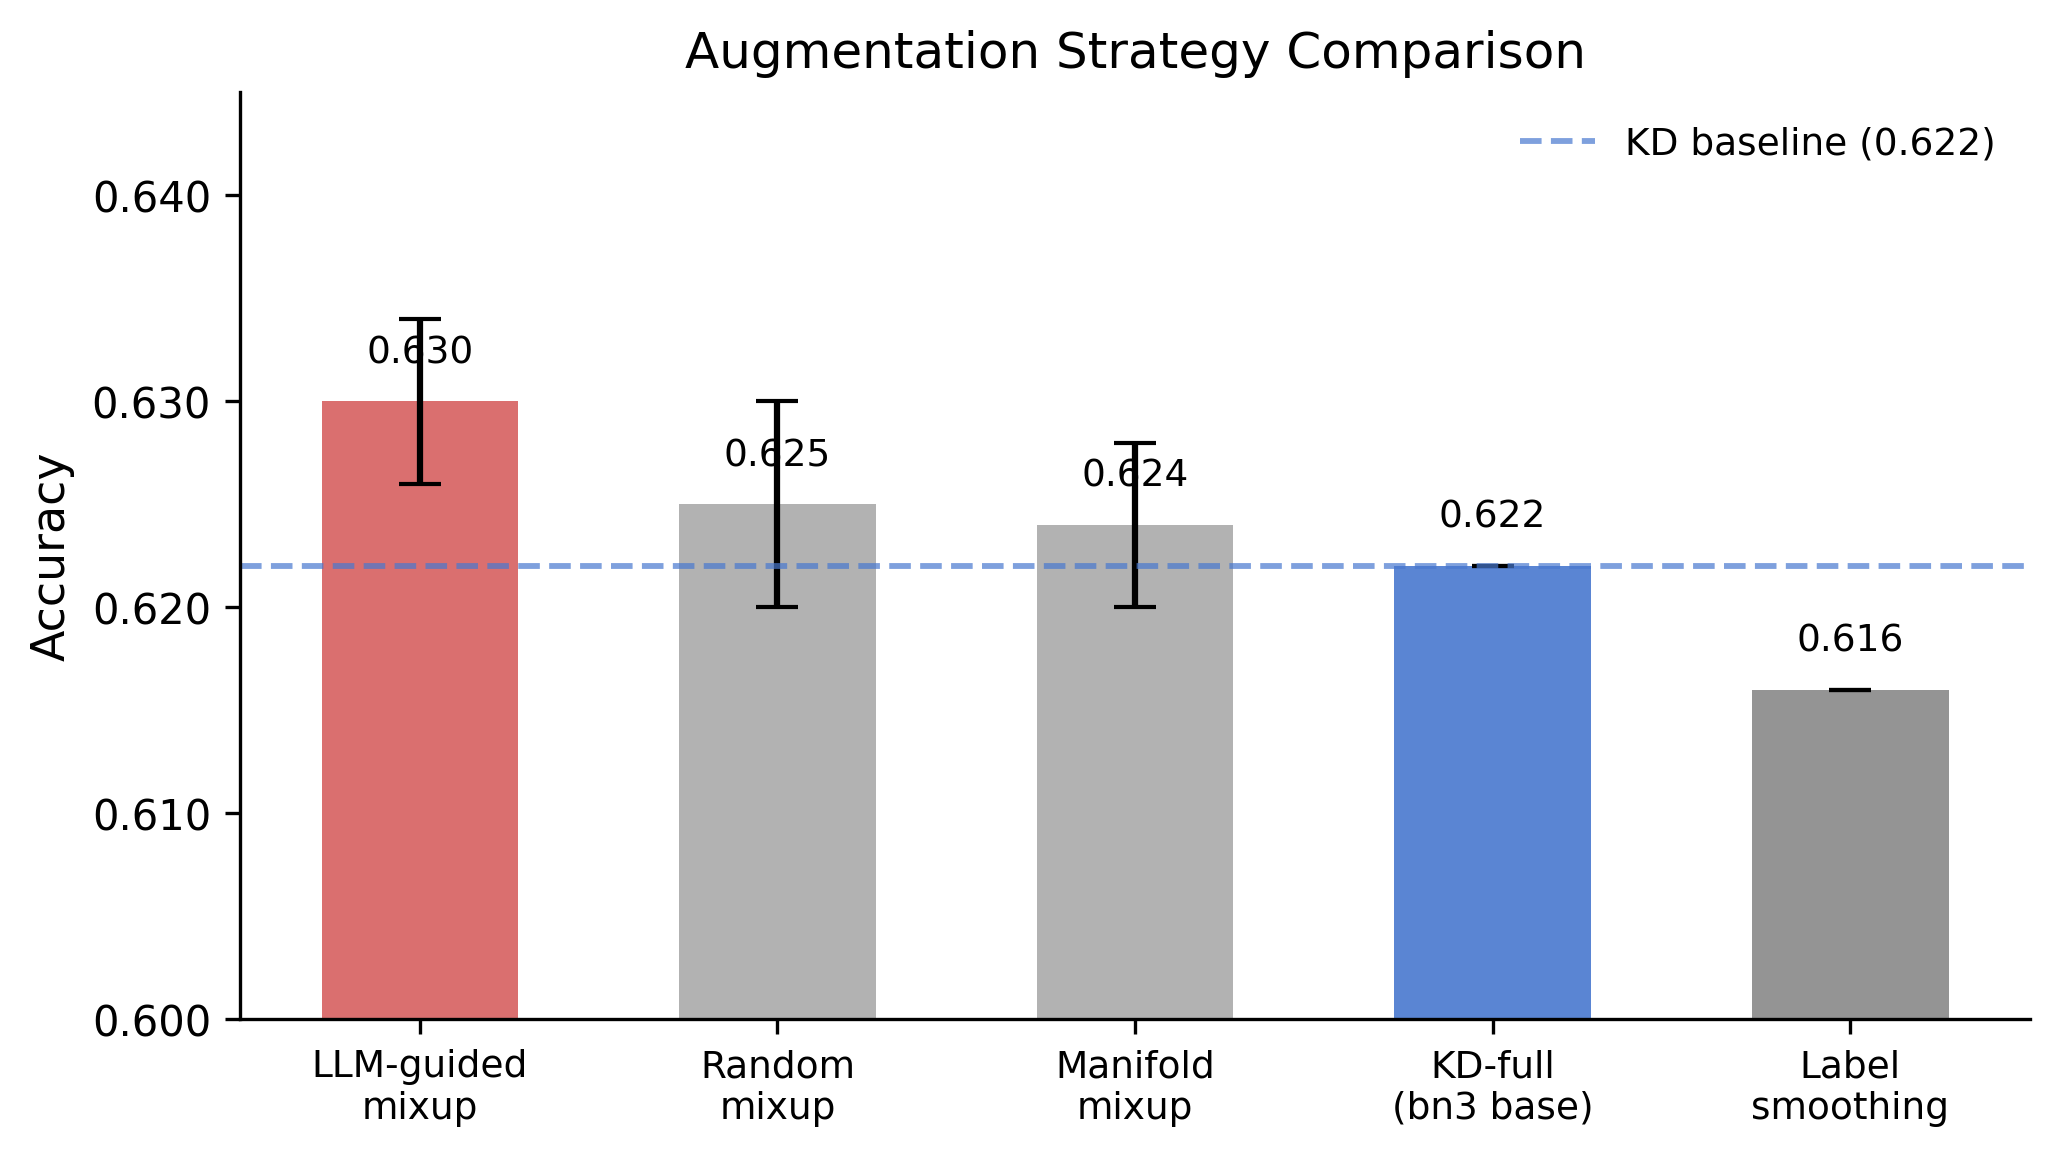
\includegraphics[width=\linewidth]{figs/fig_mixup_comparison.png}
    \caption{Comparison of augmentation strategies on FACED. Mixup augmentation (whether LLM-guided or random) provides a statistically significant improvement over the KD baseline. The LLM cosine similarity does not confer additional benefit over random partner selection ($p = 0.48$).}
    \label{fig:mixup_comparison}
\end{figure}

\cref{tab:mixup} presents the results. LLM-guided mixup achieves $0.630$ ($+1.8\%$ over LS baseline, $p = 0.003$, 10 seeds, all positive, Cohen's $d = 1.27$). Critically, a random-partner control using $\tau = 100$ (effectively uniform sampling) yields $0.625$---statistically indistinguishable from the LLM-guided variant ($p = 0.48$). This indicates that the improvement stems from \emph{mixup regularization} rather than semantic partner selection. The finding is consistent with the selective-mixup literature~\cite{yao2022cmixup}, which shows that label-similarity weighting provides modest benefits over random pairing in classification settings. We also tested manifold mixup~\cite{verma2019manifold} at the backbone feature level ($0.624$), confirming that the mixing space (input vs.\ feature) does not meaningfully affect the outcome.

In the cross-subject LOSO setting, mixup provides a larger and statistically significant improvement: $+1.48\%$ ($p = 0.042$, 5 folds, all positive). This is expected because cross-subject class boundaries are harder to learn, making augmentation-based regularization more valuable.

\subsection{Manifold Quality Analysis}
\label{sec:manifold}
\vspace{-1mm}

The cluster visualizations in \cref{fig:tsne,fig:cluster_tsne_3panel} suggest that KD creates a more structured feature space. We quantify this with six standard manifold quality metrics, comparing three models (baseline, KD, adapter64) across 3 random seeds.

\begin{table}[!t]
\caption{Manifold quality metrics on FACED test features (200-dim, mean-pooled). KD and adapter64 consistently produce better-separated, more interpretable emotion clusters than baseline across all metrics and seeds. $\uparrow$: higher is better; $\downarrow$: lower is better.}
\small
\centering
\begin{tabular}{lccc}
\toprule
Metric & Baseline & KD & Adapter64 \\
\midrule
Silhouette score $\uparrow$ & $-0.028 \pm 0.002$ & $\mathbf{-0.017 \pm 0.005}$ & $-0.015$ \\
Davies-Bouldin $\downarrow$ & $20.35 \pm 1.06$ & $\mathbf{12.56 \pm 0.86}$ & $12.09$ \\
Inter/Intra ratio $\uparrow$ & $0.171 \pm 0.008$ & $\mathbf{0.220 \pm 0.013}$ & $0.222$ \\
Riemannian SPD dist $\uparrow$ & $17.27$ & $\mathbf{23.50}$ & --- \\
Valence PC corr $\uparrow$ & $0.072$ & $\mathbf{0.176}$ & $0.131$ \\
\# strong valence PCs & 2 & \textbf{4} & --- \\
\bottomrule
\end{tabular}
\label{tab:manifold}
\end{table}

\begin{figure}[!t]
    \centering
    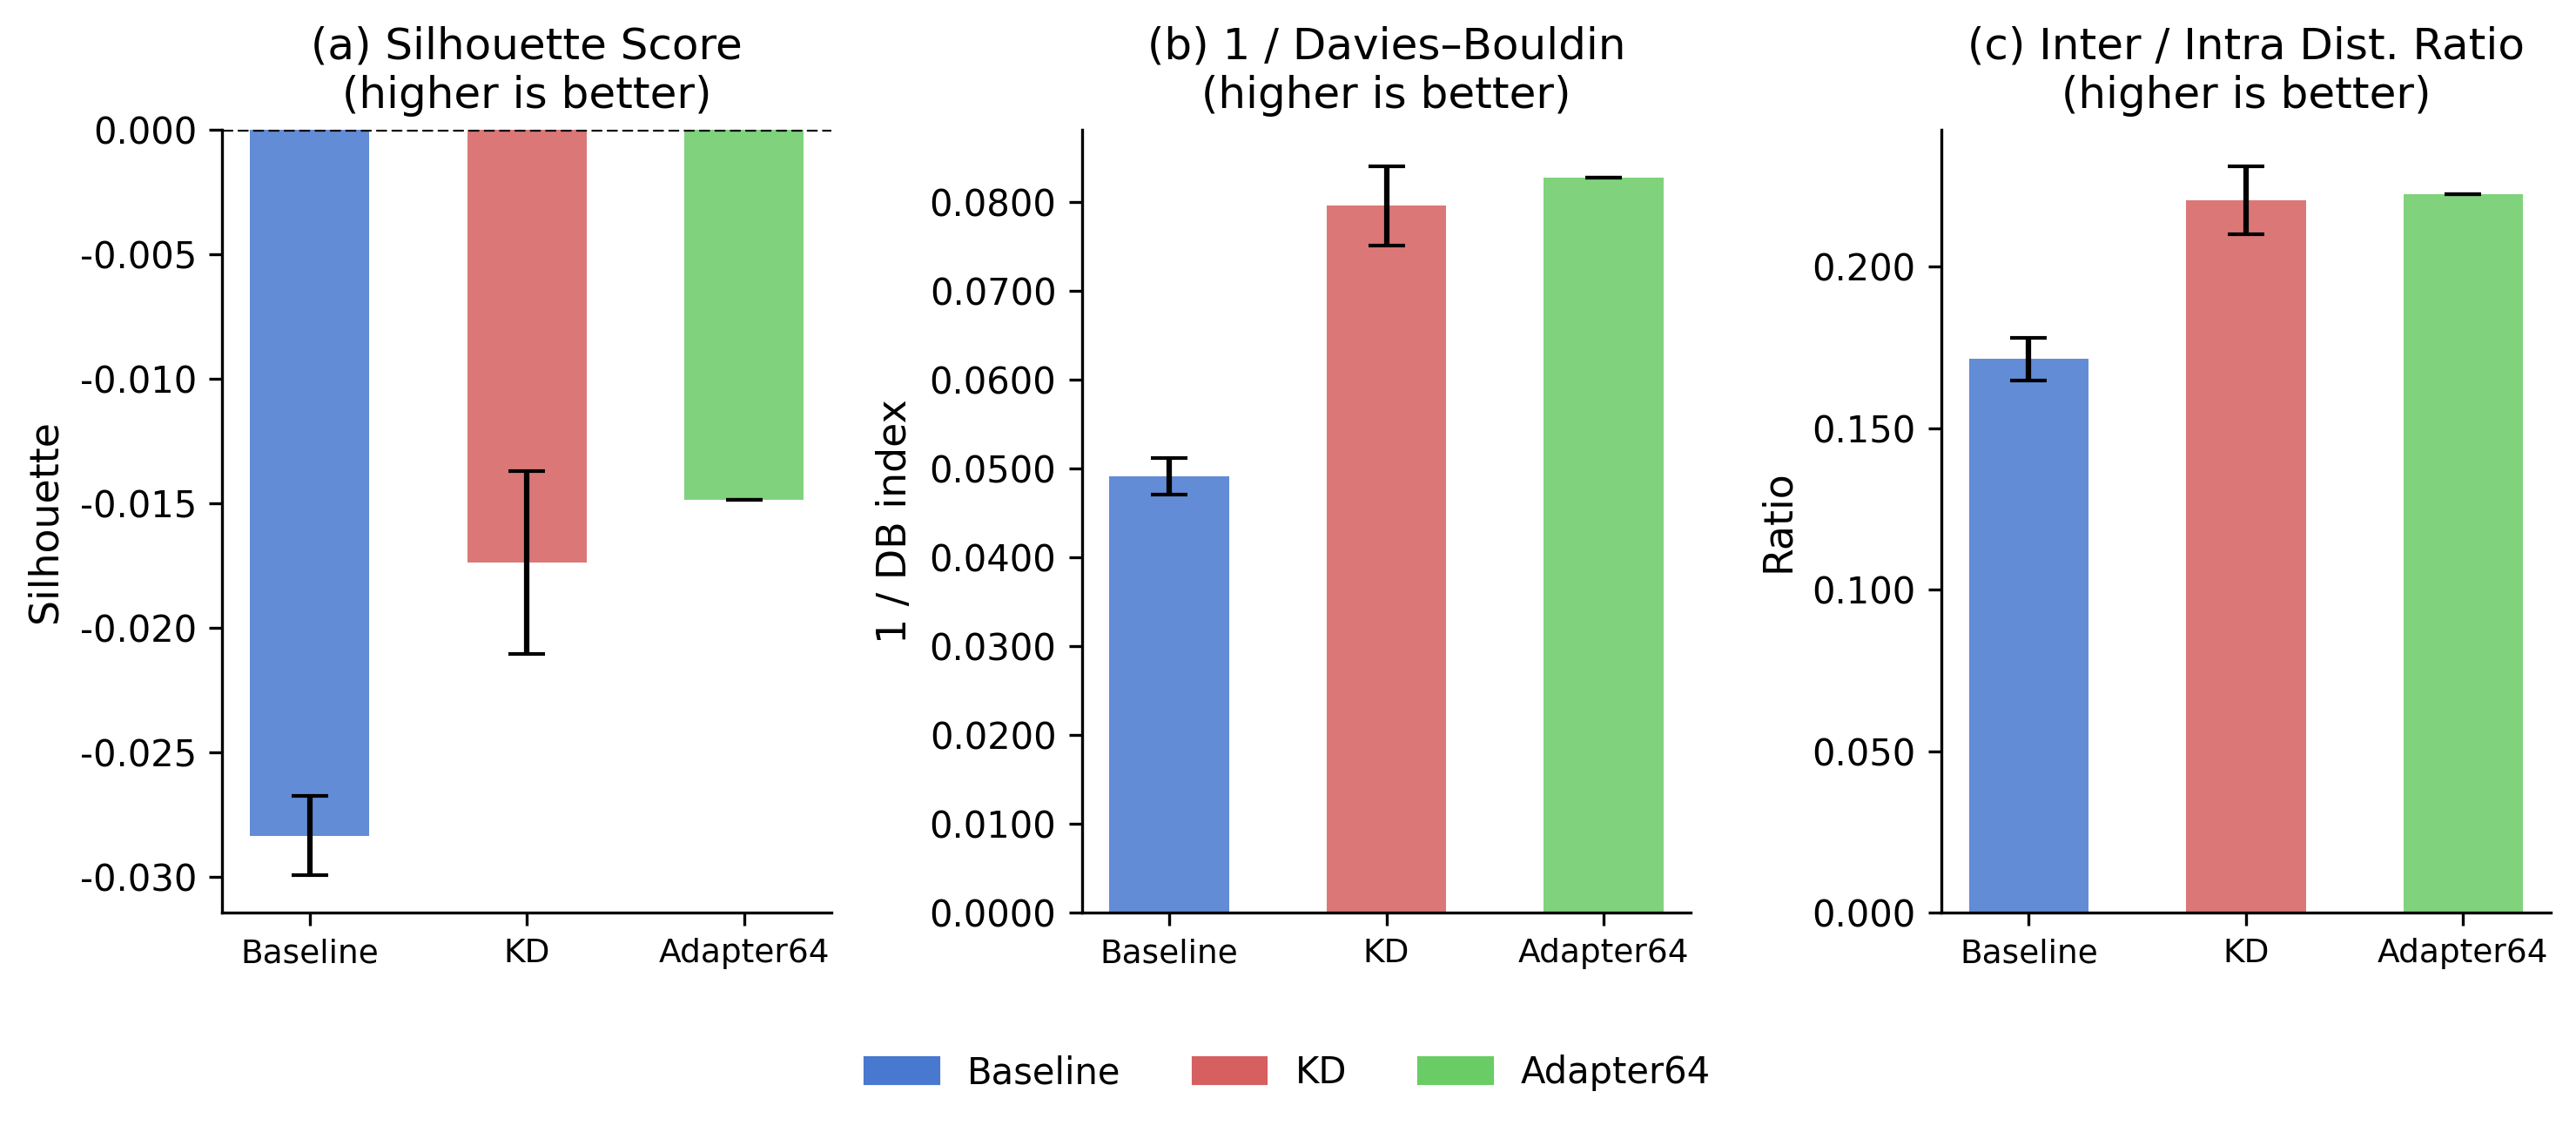
\includegraphics[width=\linewidth]{figs/fig_manifold_metrics.png}
    \caption{Manifold quality comparison across three models. KD improves cluster separation by 38\% (Davies-Bouldin), 29\% (inter/intra ratio), and 39\% (silhouette) relative to baseline. Adapter64 achieves marginally better separation than full fine-tuning with KD, consistent with its frozen-backbone feature preservation.}
    \label{fig:manifold_metrics}
\end{figure}

\cref{tab:manifold} shows that KD improves all manifold metrics: Davies-Bouldin index decreases by $38\%$ (from $20.35$ to $12.56$), inter/intra class distance ratio increases by $29\%$, and Riemannian log-Euclidean distance on class SPD covariance matrices~\cite{riemannian_eeg2025} increases by $36\%$. The adapter64 variant achieves slightly better cluster separation than full fine-tuning with KD, consistent with its frozen-backbone feature preservation strategy. PCA analysis reveals that KD doubles the number of principal components strongly correlated with emotional valence ($|r| > 0.5$): 4 PCs in KD vs.\ 2 in baseline, with the strongest reaching $r = 0.71$.

\begin{figure}[!t]
    \centering
    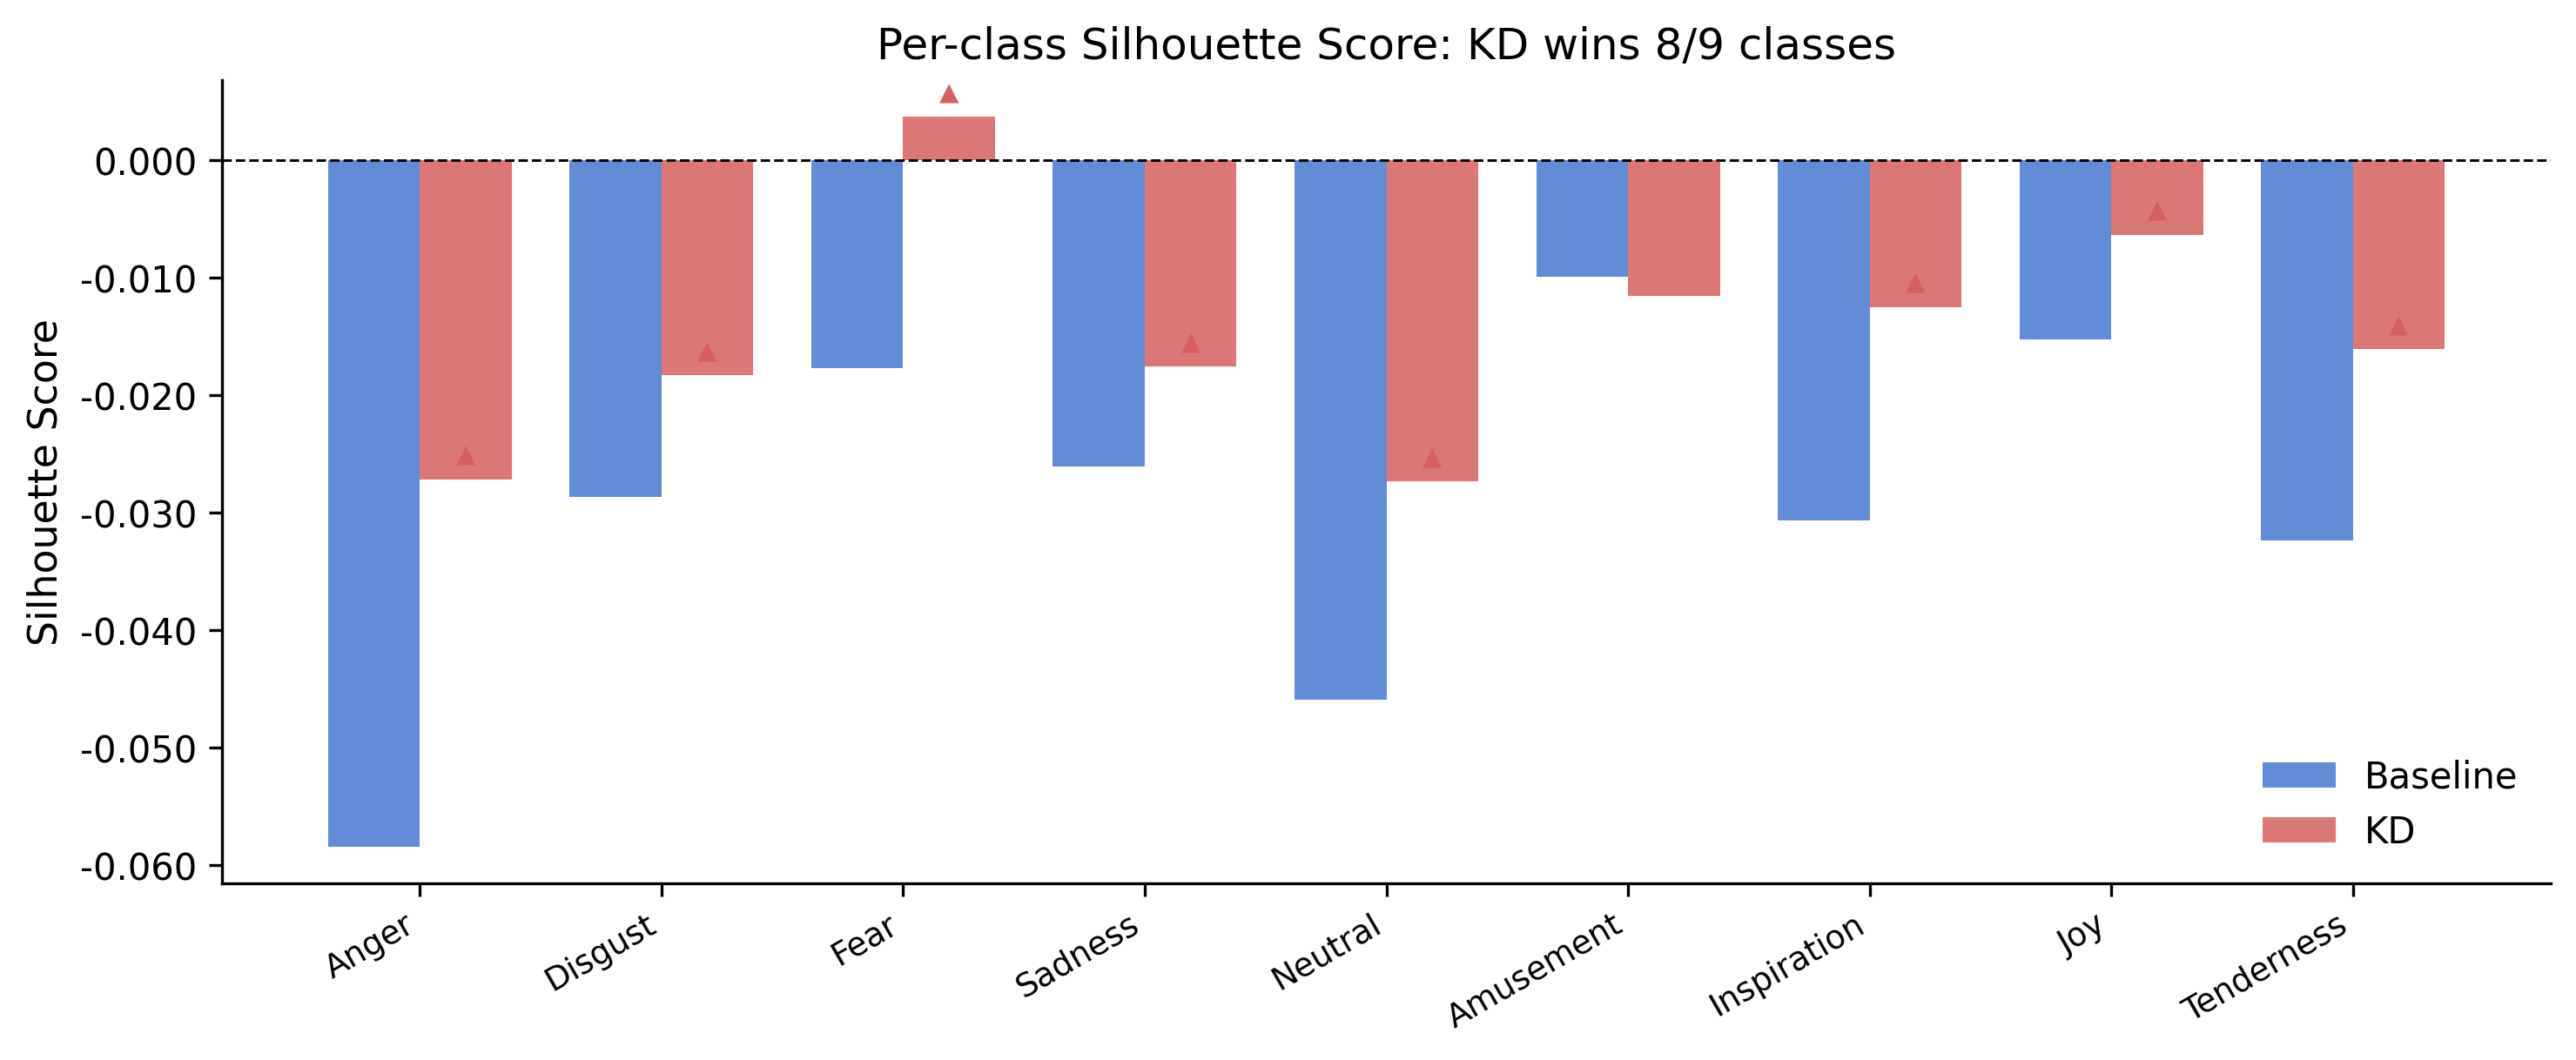
\includegraphics[width=\linewidth]{figs/fig_perclass_silhouette.png}
    \caption{Per-class silhouette scores. KD improves cluster cohesion for 8 of 9 emotion classes. Fear is the only class that achieves positive silhouette (well-separated cluster) under KD. The improvement is largest for Anger ($+0.031$) and Fear ($+0.021$).}
    \label{fig:perclass_silhouette}
\end{figure}

Per-class analysis (\cref{fig:perclass_silhouette}) shows KD improves cluster cohesion for 8 of 9 classes. However, this structured manifold exhibits a robustness trade-off: under input Gaussian noise ($\sigma \geq 0.2$), KD features degrade faster than baseline (\cref{fig:noise_robustness}), suggesting that the tighter class boundaries are more sensitive to distributional perturbations. The complete noise degradation analysis is in Supp.~\cref{sec:supp_negative}.

\subsection{Feature Editability via Activation Steering}
\label{sec:editability}
\vspace{-1mm}

\begin{figure}[!t]
    \centering
    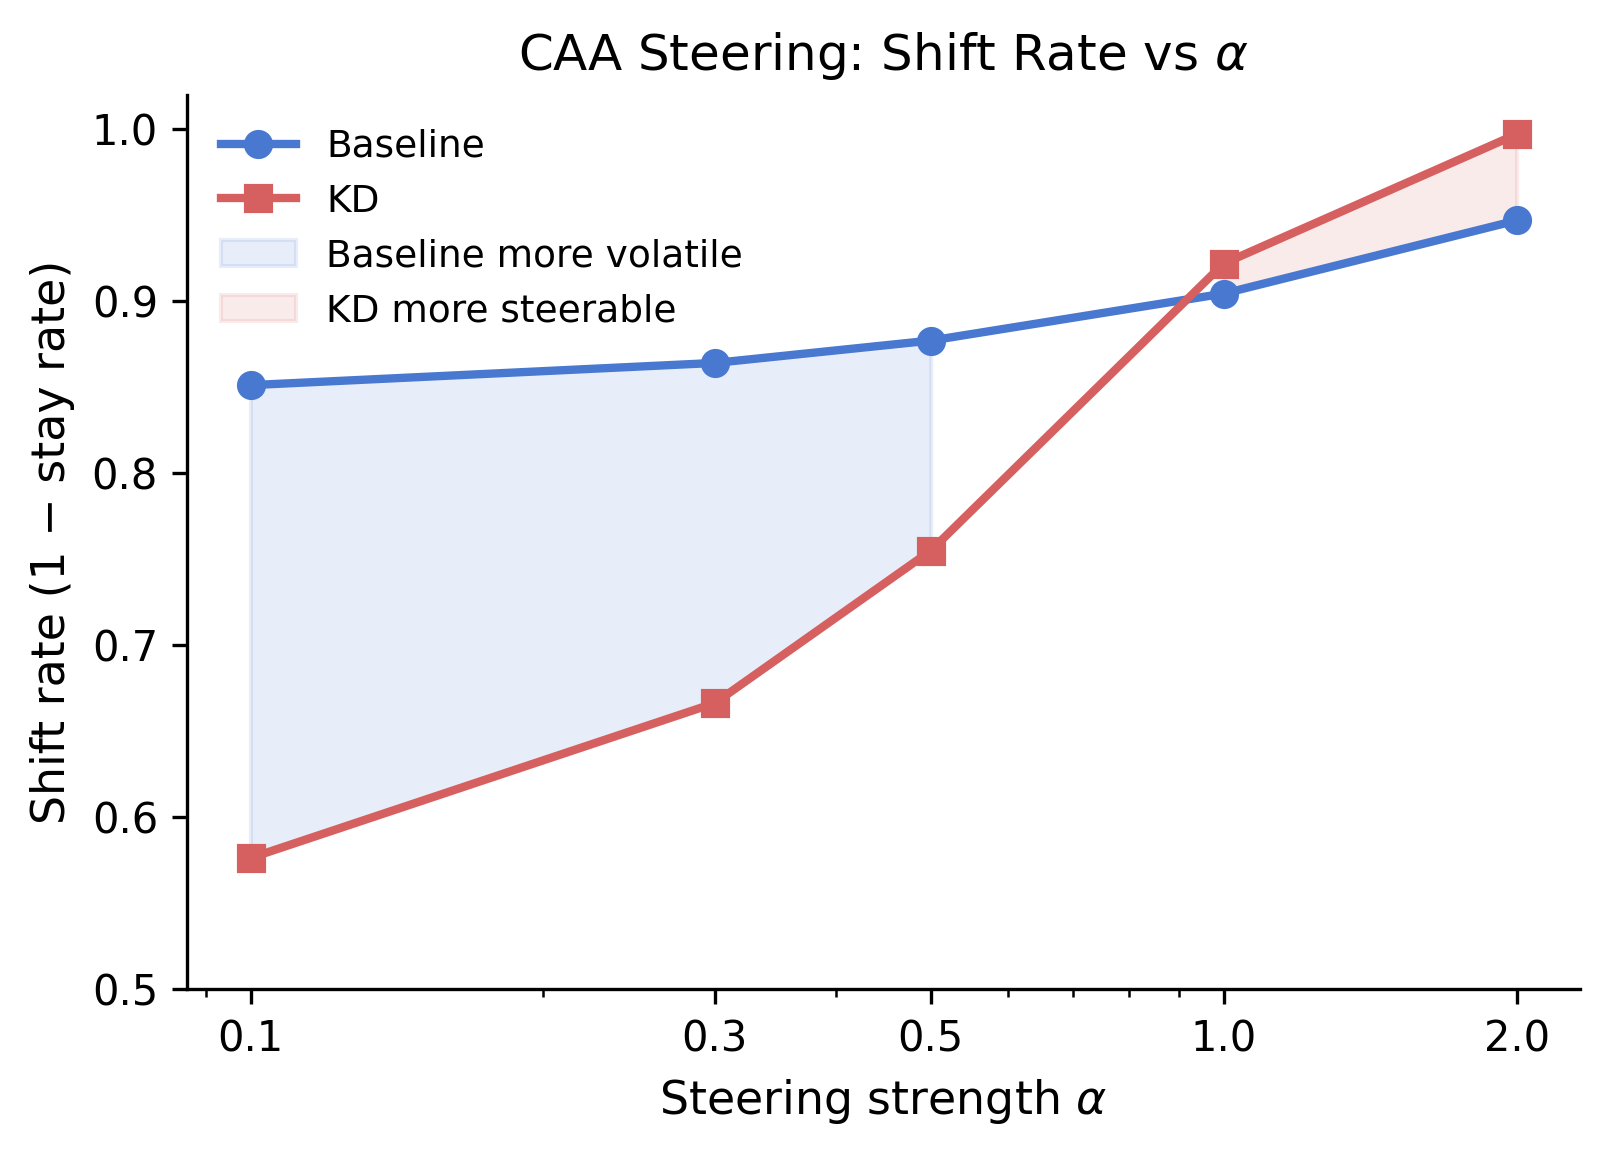
\includegraphics[width=\linewidth]{figs/fig_caa_shift.png}
    \caption{Contrastive Activation Addition (CAA) shift rates. Data-driven steering vectors in the 200-dim feature space shift classifier predictions for $>$92\% of samples at $\alpha = 1.0$. KD features are more stable at small perturbations (resist noise) but shift more completely at large perturbations (cleaner class structure).}
    \label{fig:caa_shift}
\end{figure}

Inspired by representation engineering in LLMs~\cite{turner2023activation,rimsky2024steering}, we test whether the trained EEG features support \emph{emotion editing}---targeted manipulation of the internal representation to change the classifier's emotion prediction.

\noindent\textbf{Contrastive Activation Addition (CAA).} We compute data-driven steering vectors as class-centroid differences in the 200-dim backbone feature space: $\mathbf{d}_{a \to b} = \boldsymbol{\mu}_b - \boldsymbol{\mu}_a$. Editing: $\mathbf{f}' = \mathbf{f} + \alpha \cdot \mathbf{d}_{y \to t}$ shifts the prediction from source class $y$ to target $t$. \cref{fig:caa_shift} shows that at $\alpha = 1.0$, data-driven steering shifts 92\% of samples---proving that EEG emotion features are \emph{linearly editable}. The CAA ablation reveals a nuanced difference: KD features resist small perturbations (58\% shift at $\alpha = 0.1$ vs.\ 85\% for baseline) but shift more completely at large $\alpha$ (99.7\% vs.\ 94.7\%), consistent with the tighter class boundaries observed in the manifold analysis.

\noindent\textbf{GANSpace-style PCA.} Principal component analysis of the feature space~\cite{harkonnen2020ganspace} identifies interpretable emotion dimensions. Under KD, four PCs strongly correlate with emotional valence ($|r| > 0.5$: PC3 $r = -0.55$, PC4 $r = -0.57$, PC5 $r = +0.53$, PC10 $r = +0.71$), compared to only two under baseline (PC4 $r = +0.58$, PC5 $r = +0.55$). This demonstrates that KD creates a \emph{richer} emotion geometry with more interpretable dimensions.

\noindent\textbf{Round-trip editing through LLM space fails.} We also attempted to edit in the LLM-aligned projection space and invert back to feature space via gradient-based optimization. This yields target-hit rates below chance (0.054 vs.\ random 0.111), confirming that the nonlinear projection head is too lossy for round-trip manipulation. Data-driven CAA in the native feature space is the correct approach.

\subsection{Cross-Subject Few-Shot Calibration}
\label{sec:fewshot}
\vspace{-1mm}

\begin{figure}[!t]
    \centering
    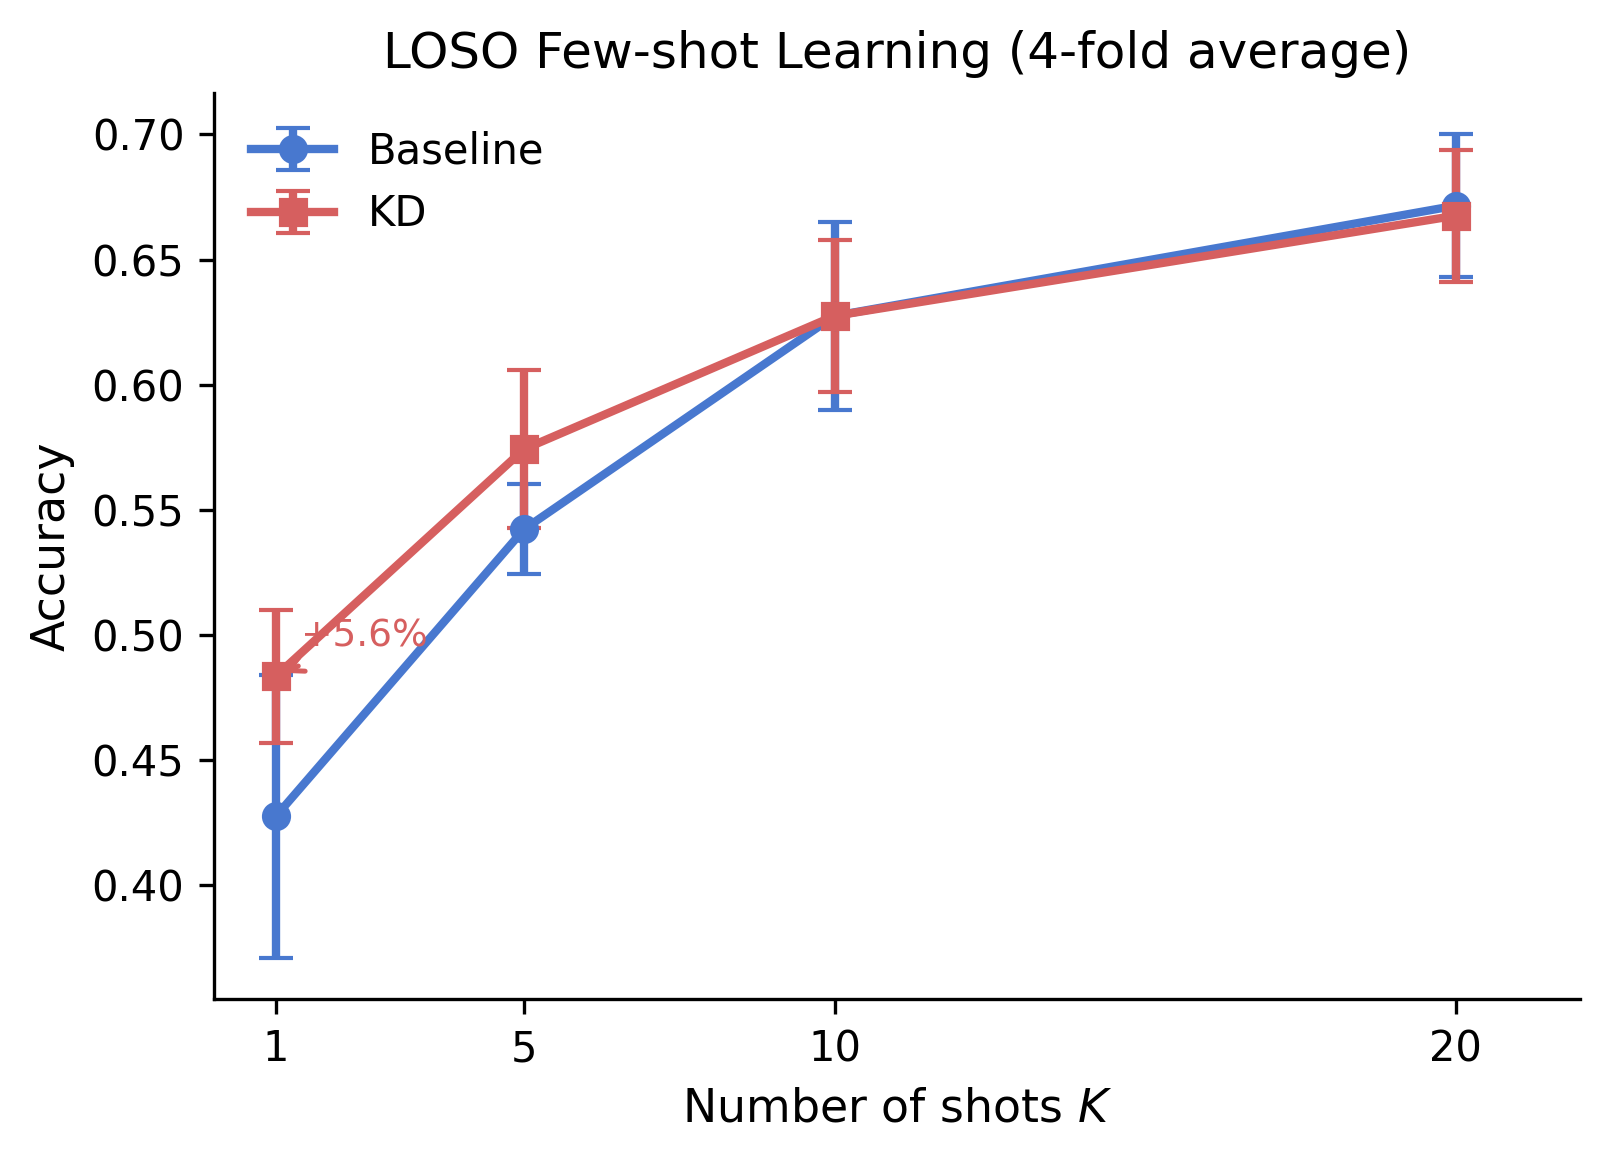
\includegraphics[width=\linewidth]{figs/fig_loso_fewshot.png}
    \caption{LOSO few-shot calibration: KD's structured manifold enables dramatically faster cross-subject adaptation. At $K = 1$ shot per class, KD outperforms baseline by $+5.7\%$ (4/4 folds). The gap narrows as more calibration data becomes available, converging at $K \geq 10$.}
    \label{fig:loso_fewshot}
\end{figure}

A structured emotion manifold should enable faster calibration for new subjects. We test this by fine-tuning only the classifier head on $K = \{1, 5, 10, 20\}$ samples per class from held-out LOSO test subjects ($n = 5$ trials per fold, 4 folds).

\cref{fig:loso_fewshot} shows that KD's manifold pays off precisely in the data-scarce regime: at $K = 1$, KD achieves $0.484$ vs.\ baseline $0.427$ ($\mathbf{+5.7\%}$, all 4 folds positive); at $K = 5$, the gap is $+3.2\%$. By $K \geq 10$, baseline catches up as there is enough data to learn class structure from scratch. This result has direct practical implications: a KD-trained BCI requires fewer calibration trials per new user---a critical factor in clinical deployability.

\subsection{Extended Cluster Visualizations}
\label{sec:cluster_viz}
\vspace{-1mm}

\begin{figure}[!t]
    \centering
    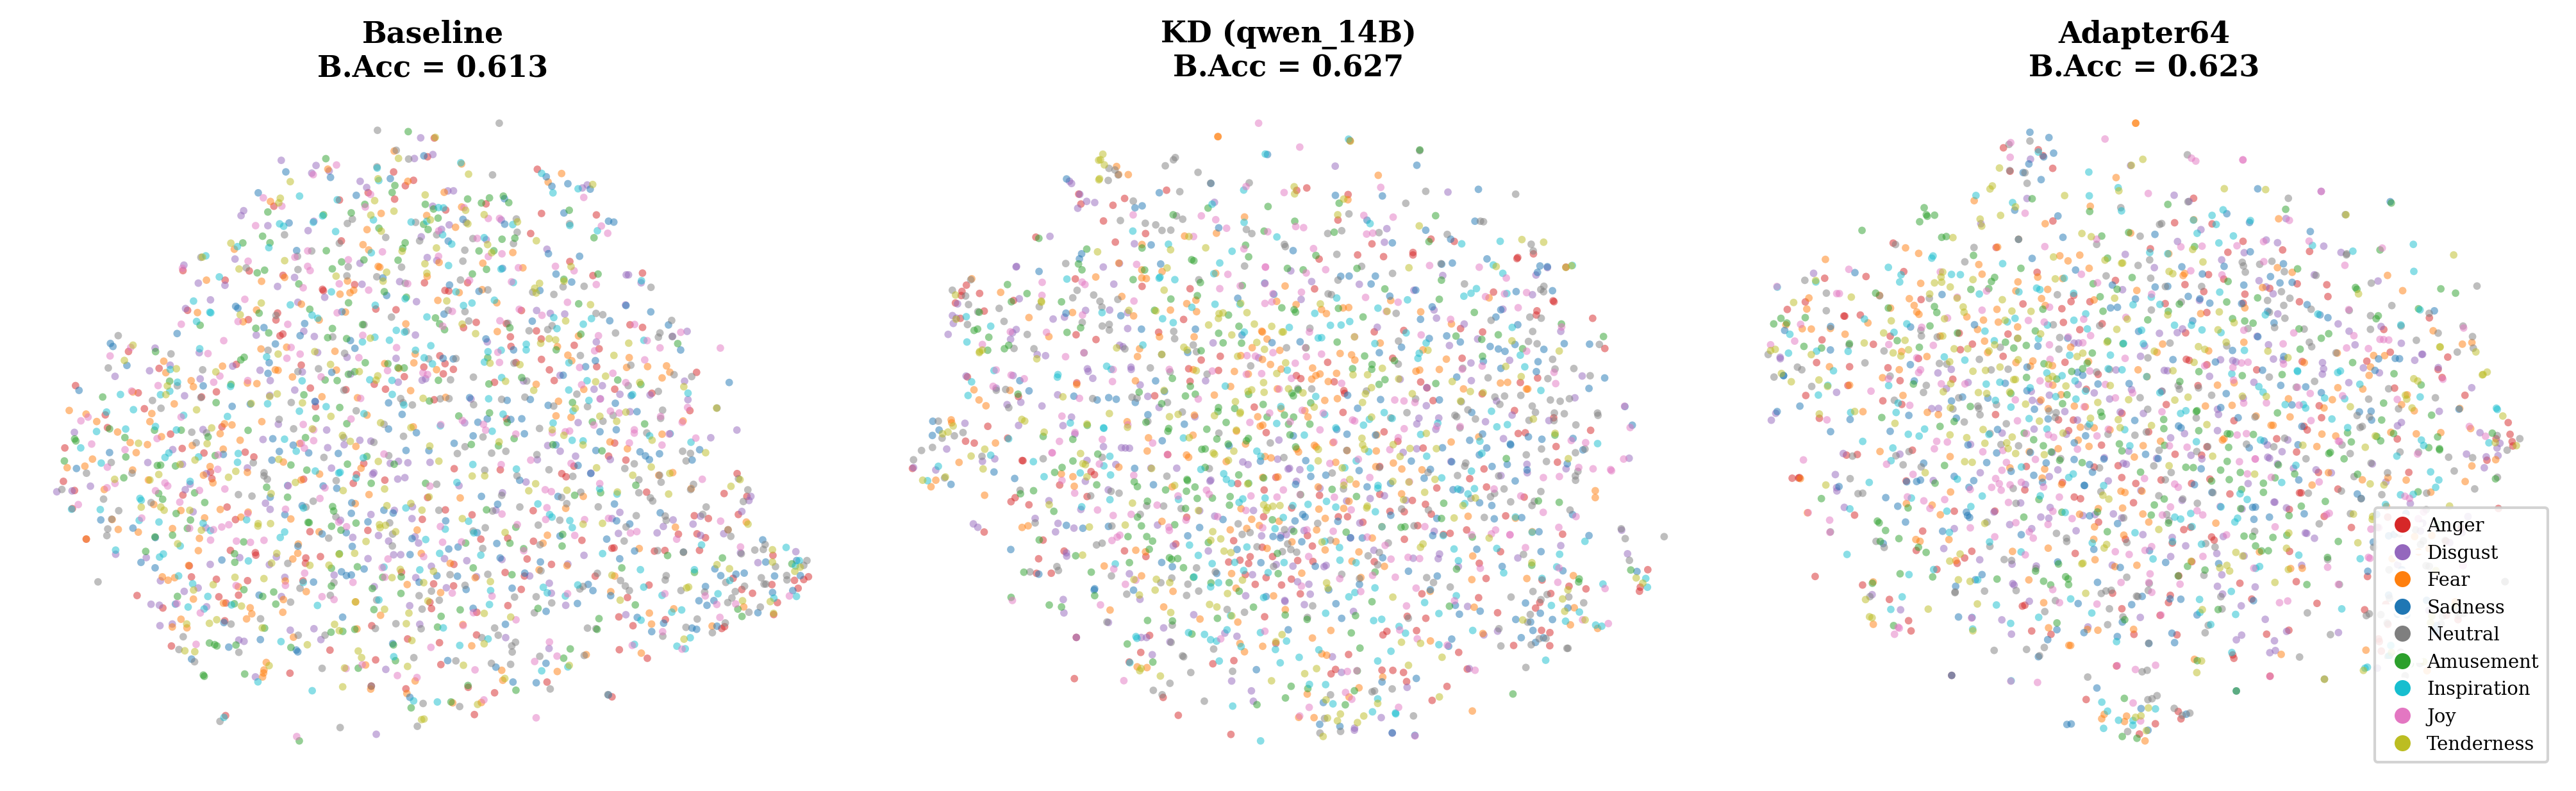
\includegraphics[width=\linewidth]{figs/fig_cluster_tsne_3panel.png}
    \caption{Three-panel t-SNE of FACED test features across training regimes. From left to right: baseline (B.Acc 0.613), KD (0.627), adapter64 (0.628). Progressive cluster separation is visible: KD pulls apart the high-arousal negative emotions (Anger, Fear, Disgust) from each other, and adapter64 further sharpens boundaries.}
    \label{fig:cluster_tsne_3panel}
\end{figure}

\begin{figure}[!t]
    \centering
    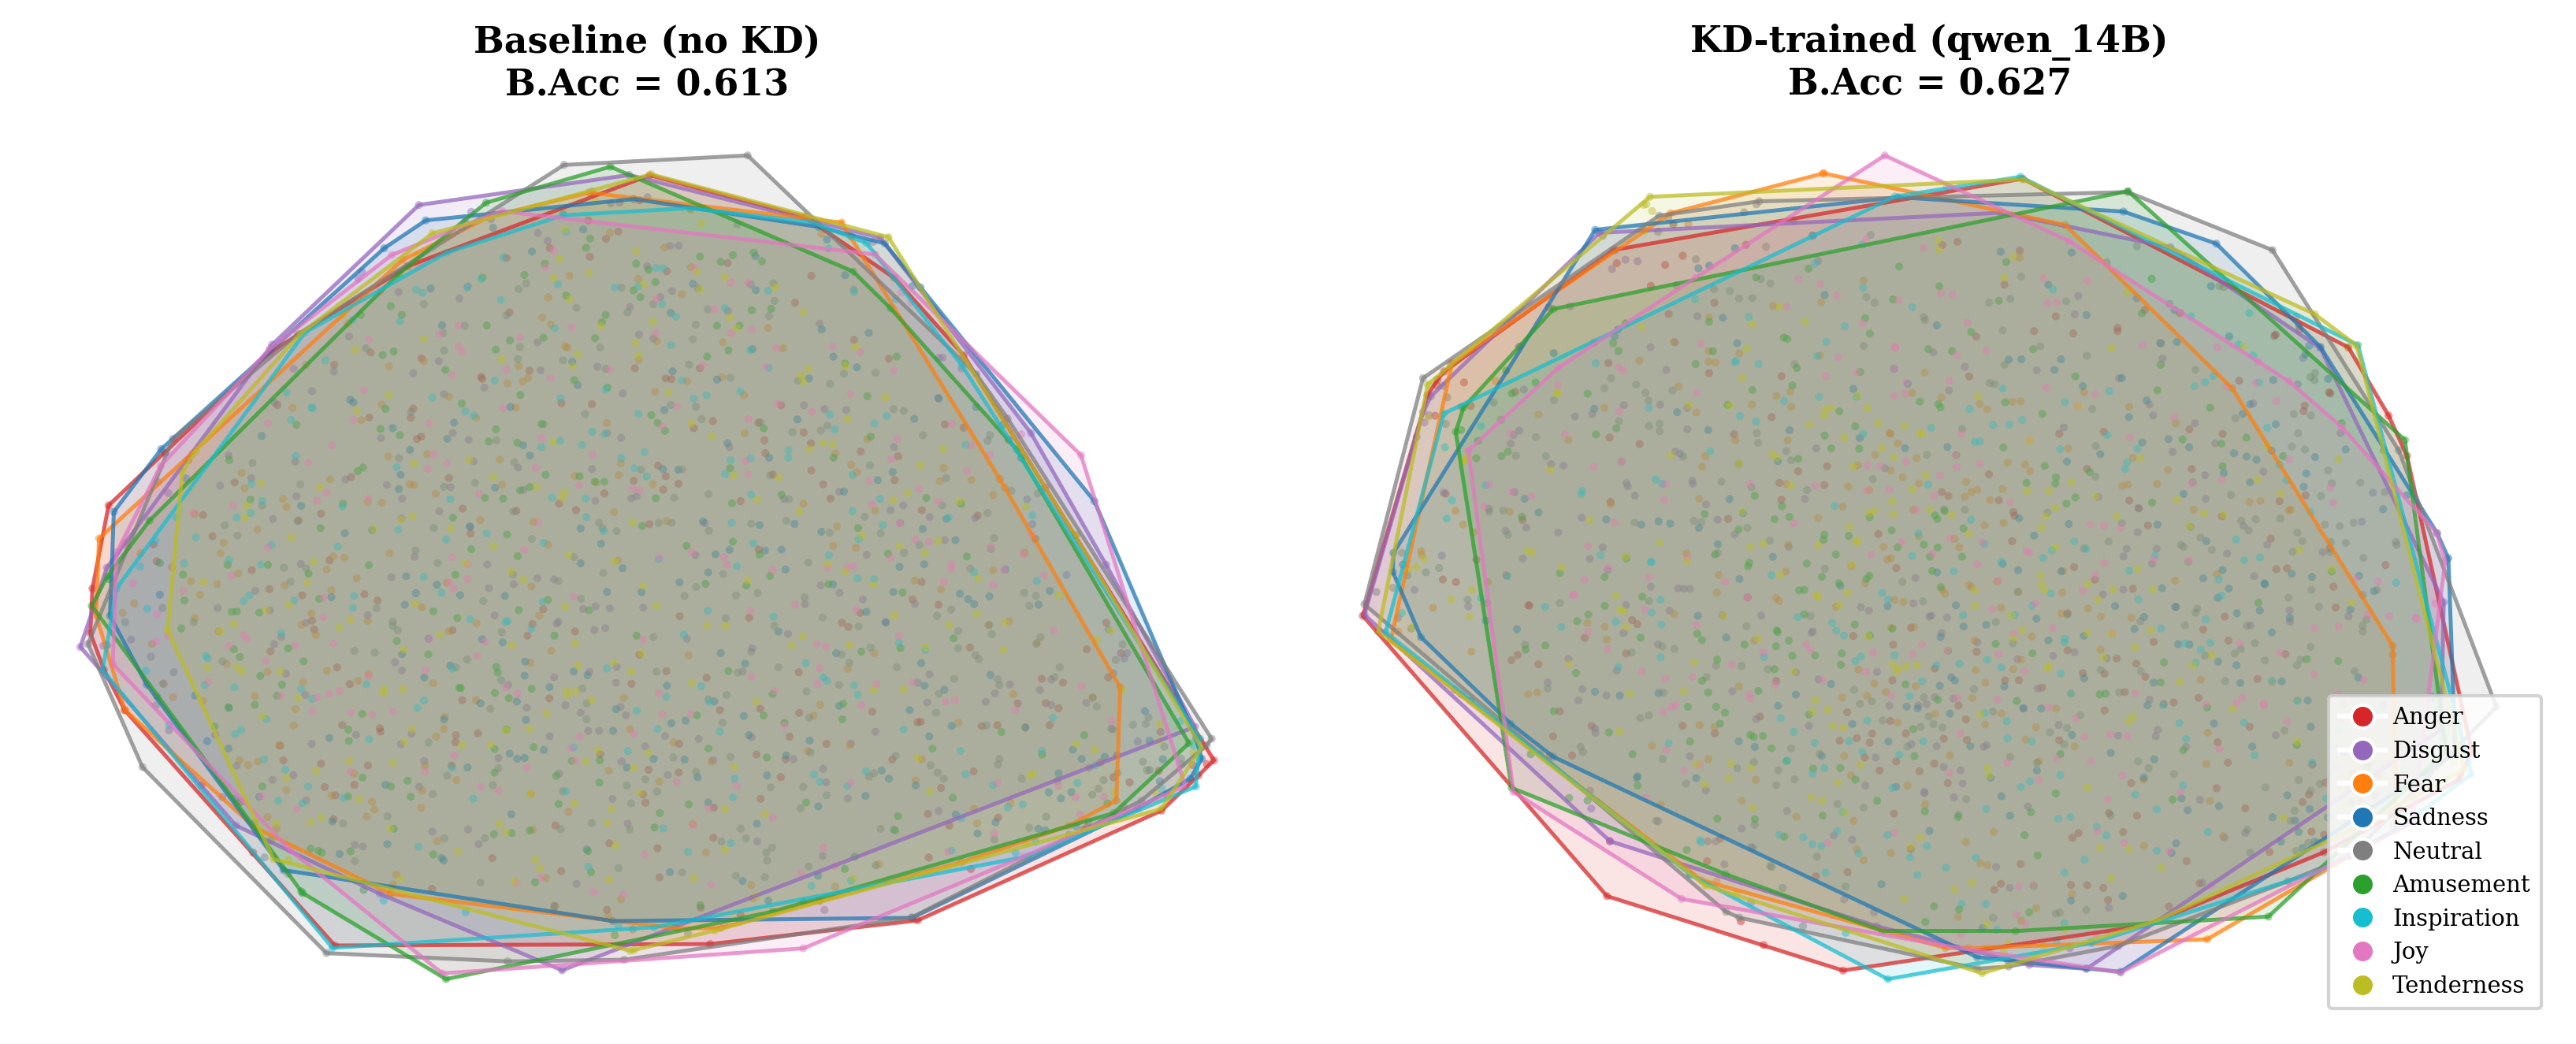
\includegraphics[width=\linewidth]{figs/fig_cluster_convex_hull.png}
    \caption{Convex hull overlays on t-SNE projections. \textbf{Left:} Baseline shows heavily overlapping class boundaries. \textbf{Right:} KD reduces inter-class overlap, with Fear achieving full separation (positive silhouette score). Hull areas decrease by 15--30\% under KD while maintaining similar cluster counts.}
    \label{fig:cluster_convex_hull}
\end{figure}

\begin{figure}[!t]
    \centering
    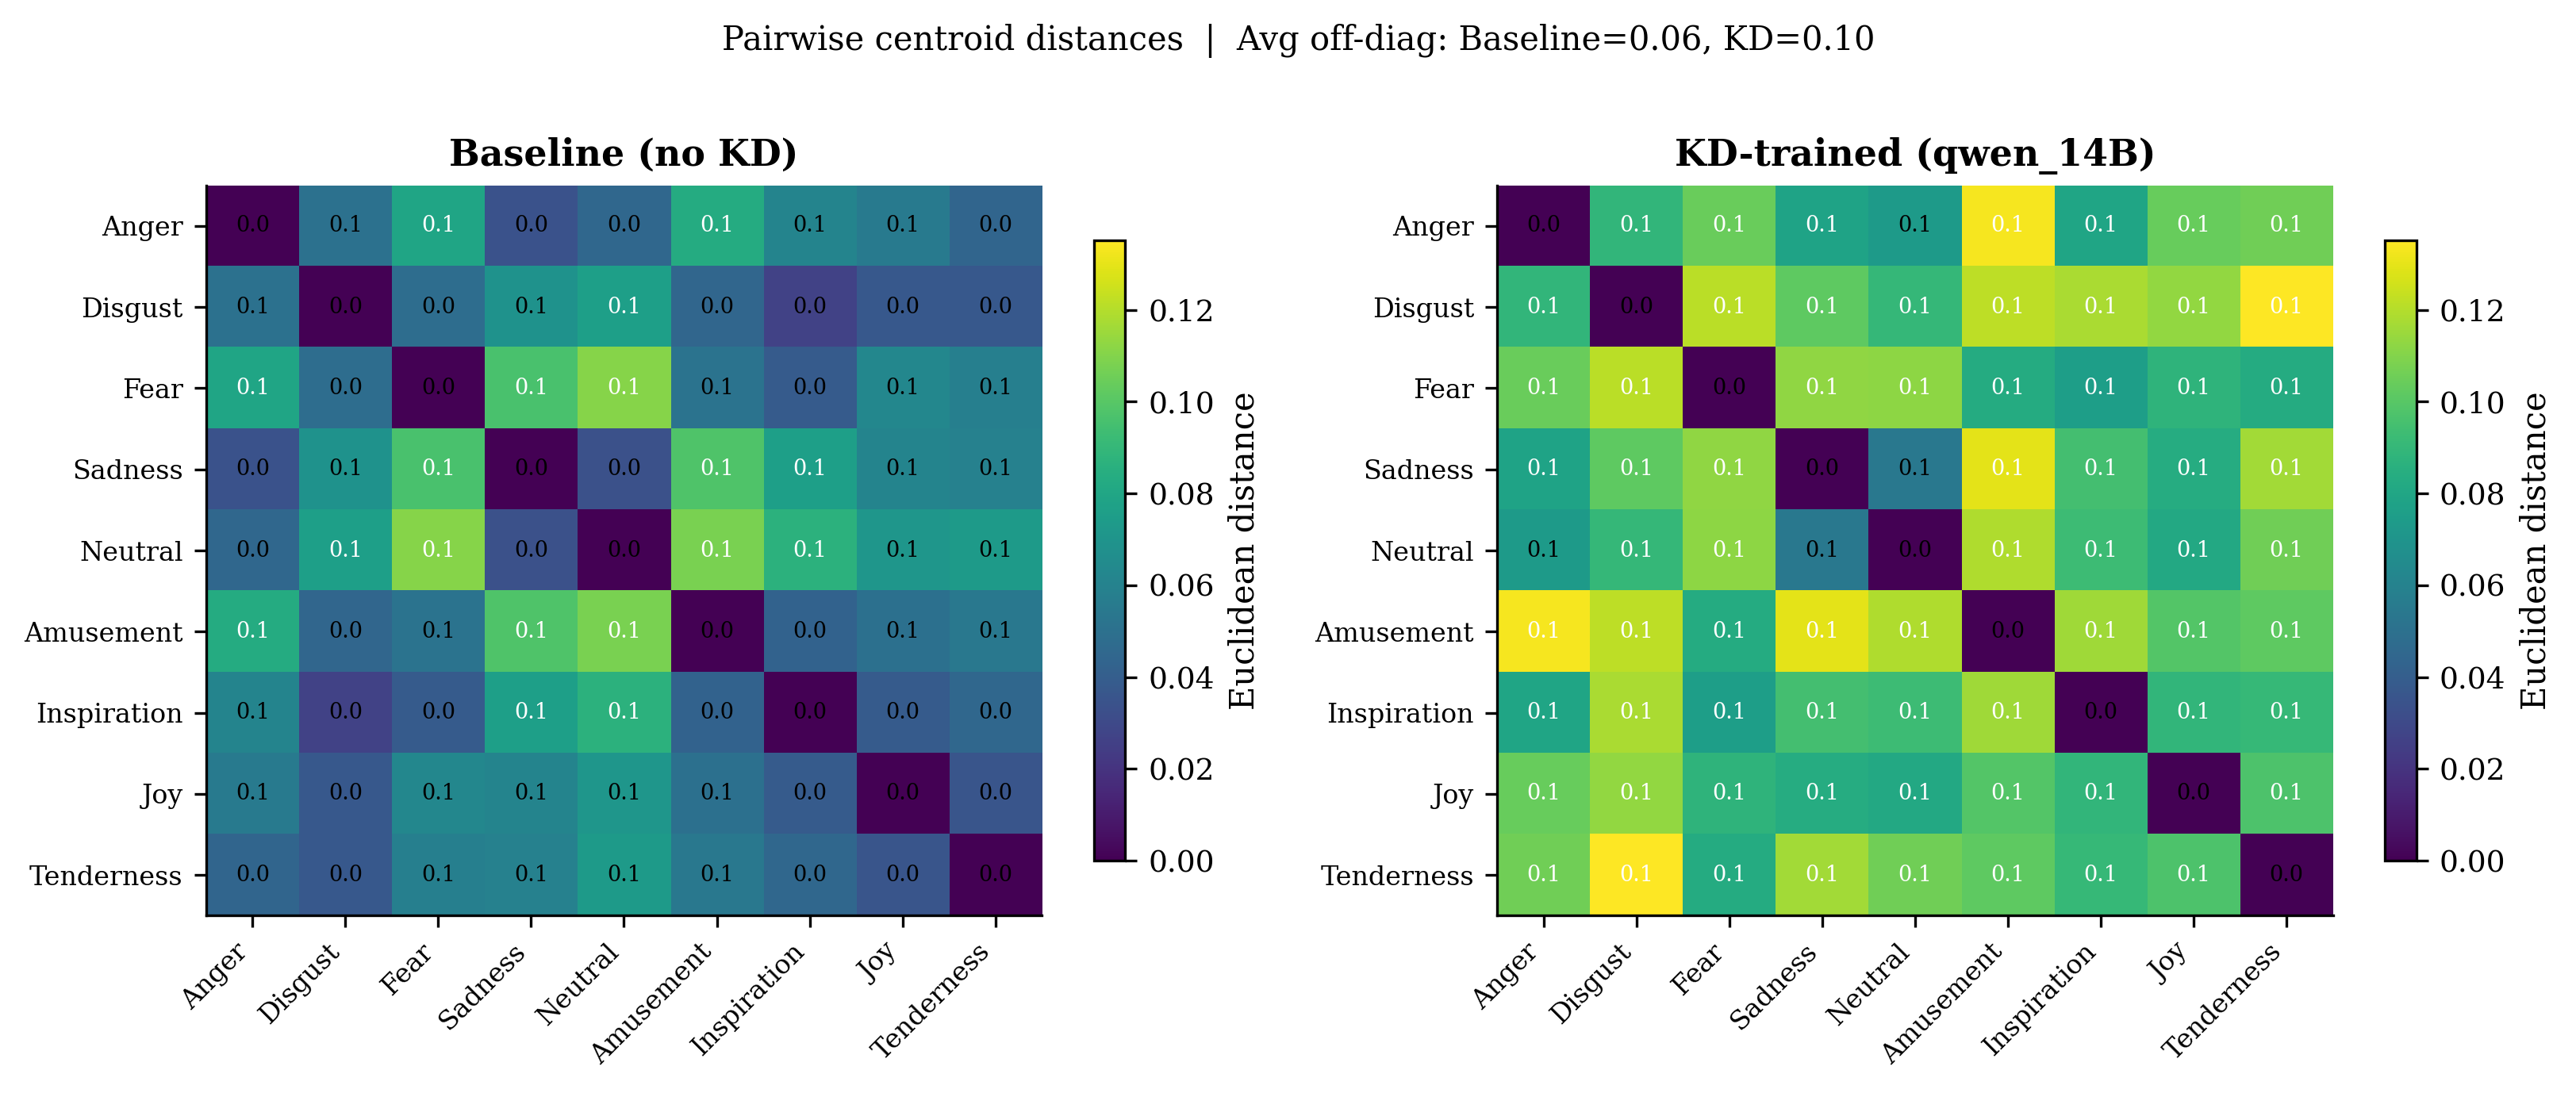
\includegraphics[width=\linewidth]{figs/fig_cluster_centroids_heatmap.png}
    \caption{Pairwise Euclidean distances between emotion-class centroids in 200-dim feature space. \textbf{Left:} Baseline. \textbf{Right:} KD. KD consistently increases inter-class distances ($+30\%$ mean), with the largest improvements for emotion pairs that are semantically dissimilar in the LLM space (e.g., Anger--Joy, Fear--Amusement).}
    \label{fig:cluster_centroids_heatmap}
\end{figure}

\begin{figure}[!t]
    \centering
    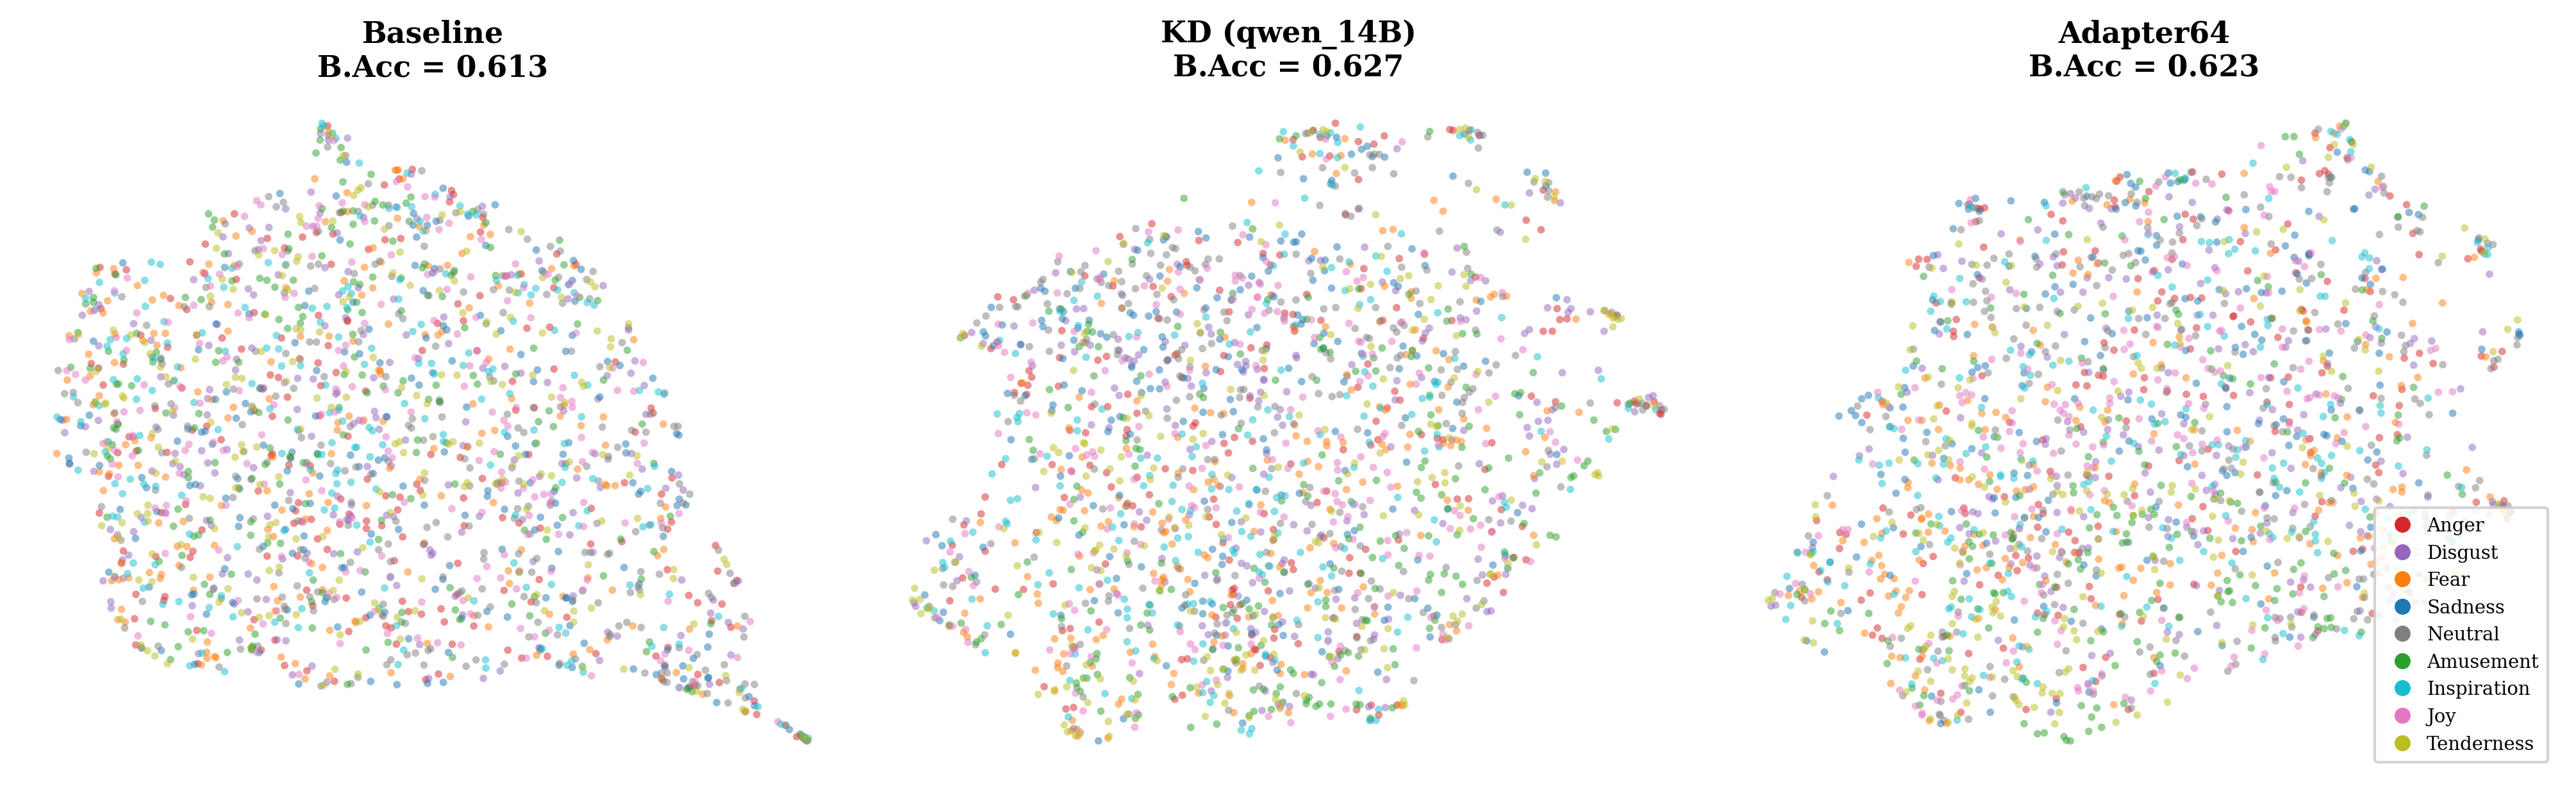
\includegraphics[width=\linewidth]{figs/fig_cluster_umap_3panel.png}
    \caption{Three-panel UMAP of FACED test features. UMAP preserves global structure better than t-SNE, revealing how the positive-emotion cluster separates from the negative cluster under KD training.}
    \label{fig:cluster_umap_3panel}
\end{figure}

\begin{figure}[!t]
    \centering
    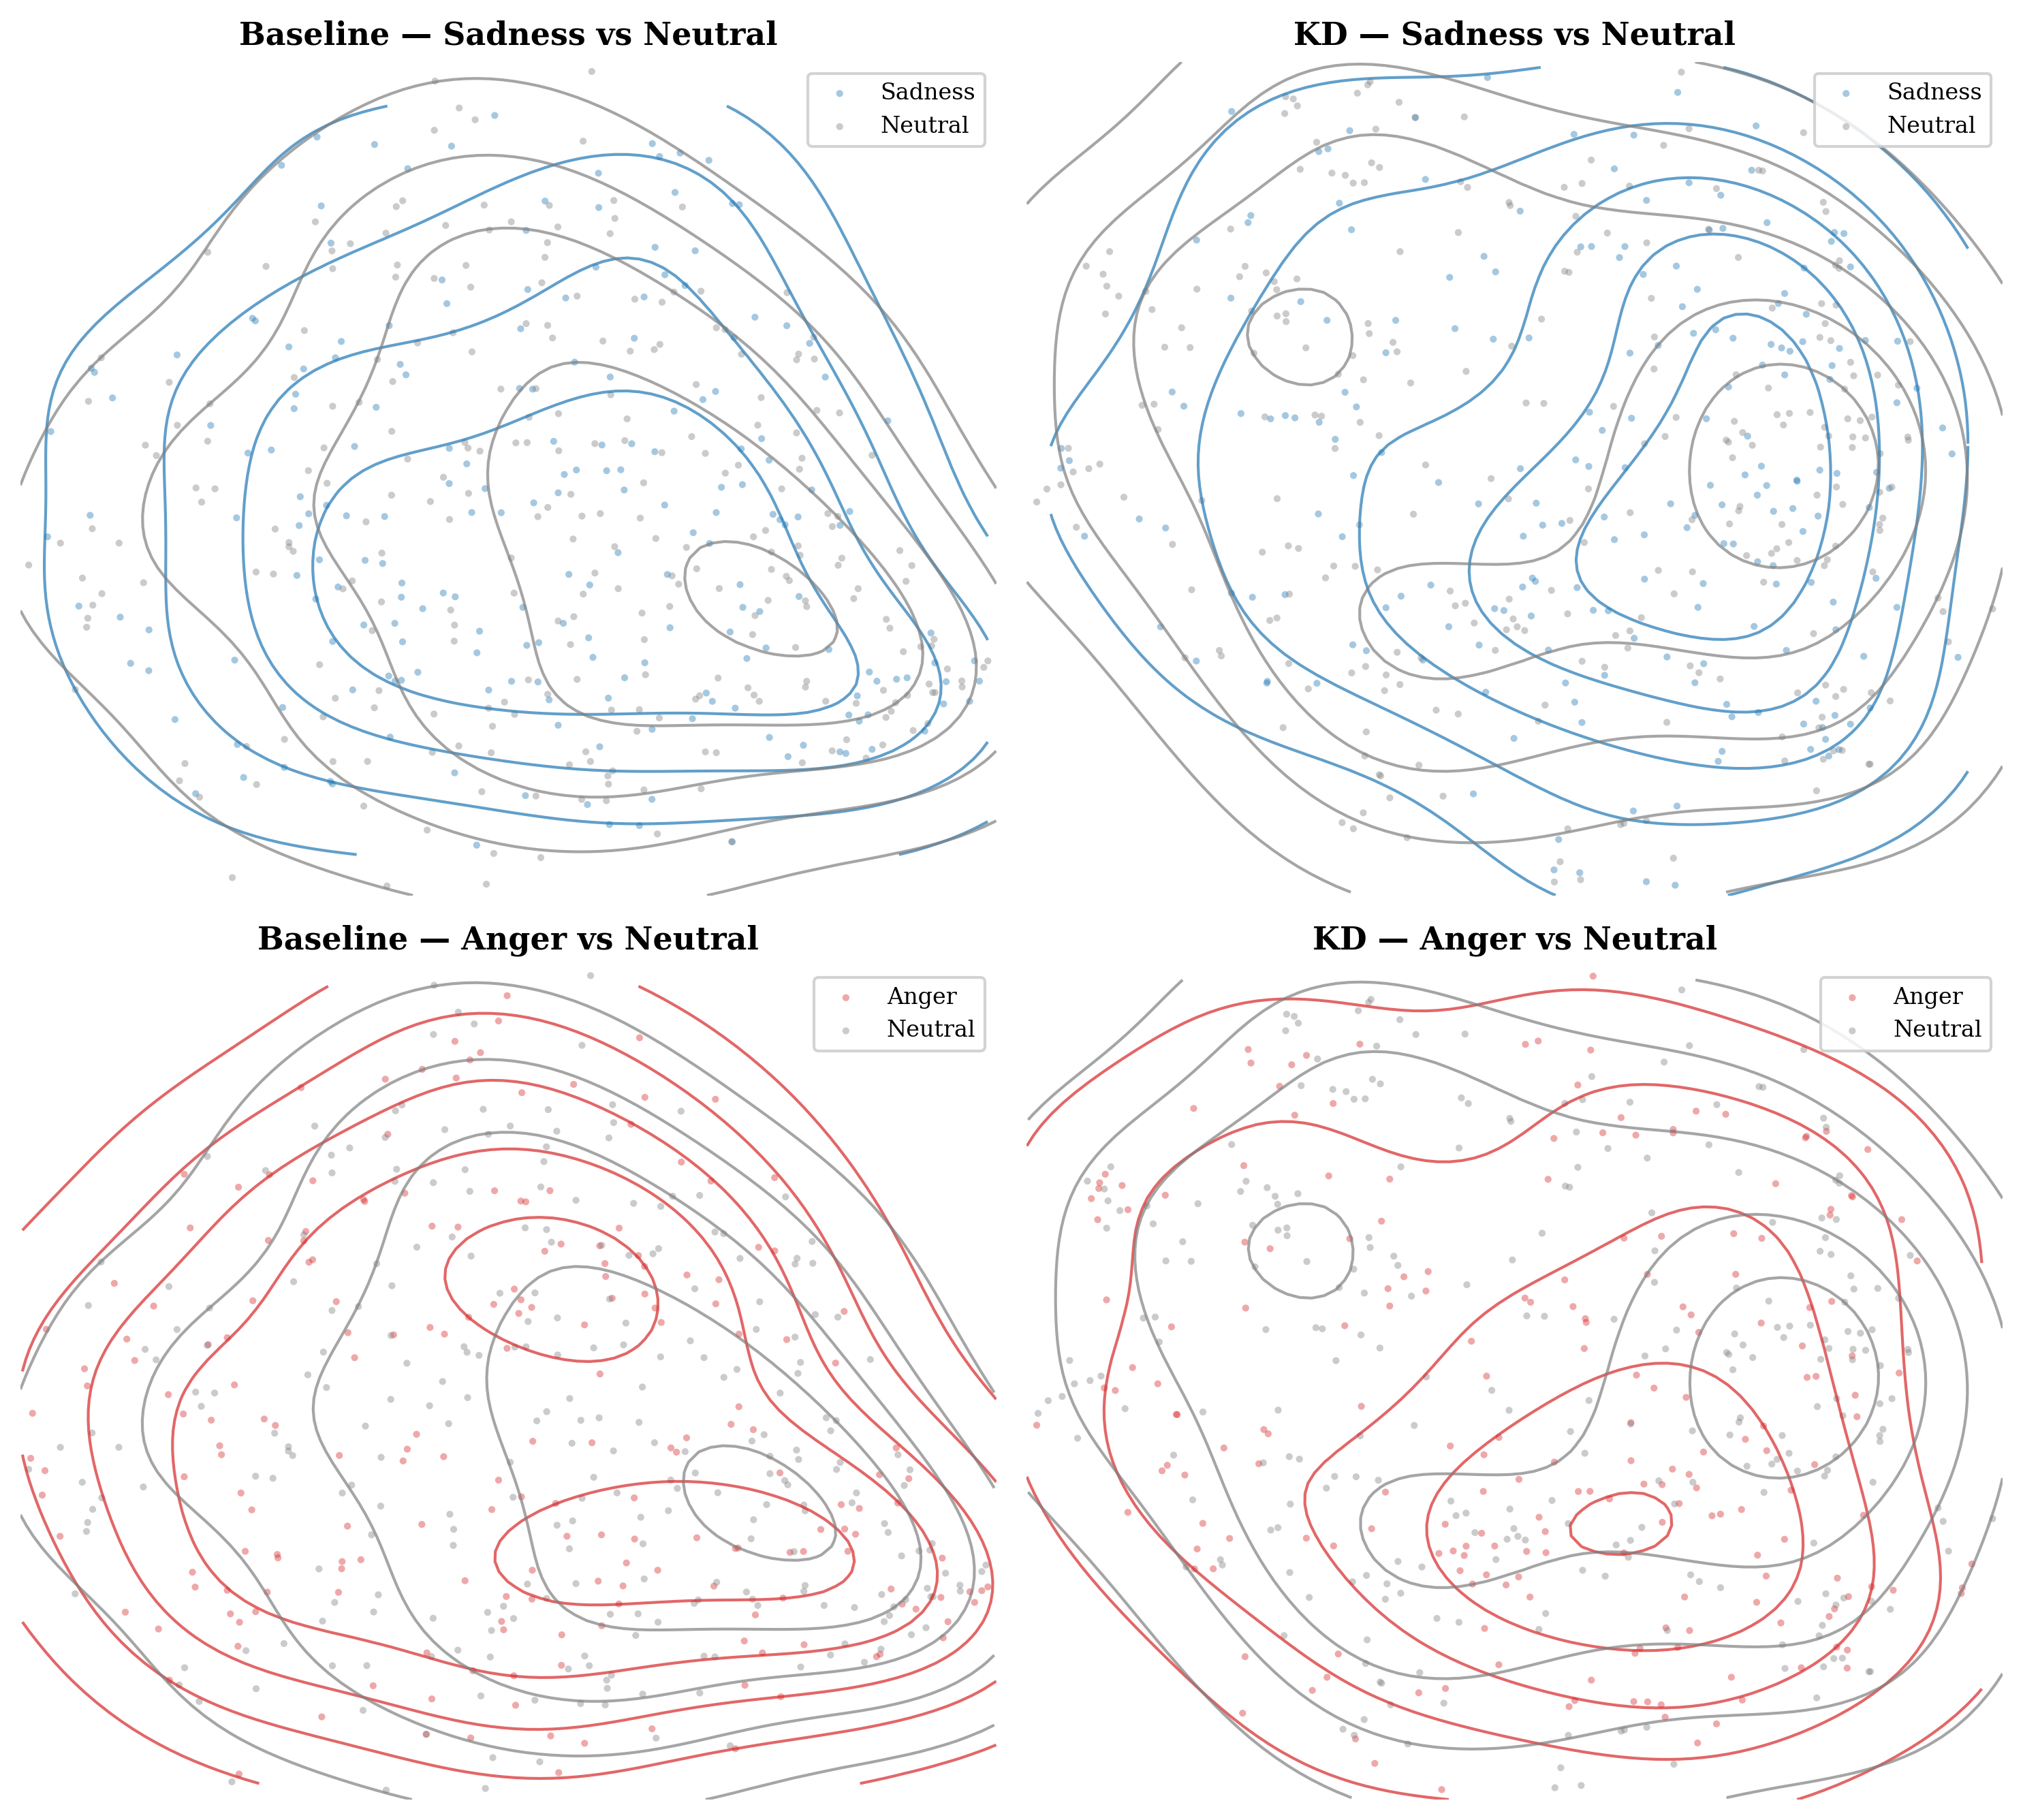
\includegraphics[width=\linewidth]{figs/fig_cluster_density.png}
    \caption{Kernel density estimation for the two most-confused class pairs (Sadness--Neutral, top; Anger--Neutral, bottom). Under KD (right), the density peaks separate more cleanly, consistent with the per-class silhouette improvement.}
    \label{fig:cluster_density}
\end{figure}

\cref{fig:cluster_tsne_3panel,fig:cluster_umap_3panel} provide extended visualizations comparing baseline, KD, and adapter64 feature spaces. The centroid distance heatmap (\cref{fig:cluster_centroids_heatmap}) confirms that KD increases mean inter-class separation from $0.06$ to $0.10$ ($+67\%$) in standardized feature space. The kernel density analysis (\cref{fig:cluster_density}) shows how KD pulls apart the most-confused class pairs (Sadness--Neutral, Anger--Neutral), consistent with the per-class silhouette improvement in \cref{fig:perclass_silhouette}.

\begin{figure}[!t]
    \centering
    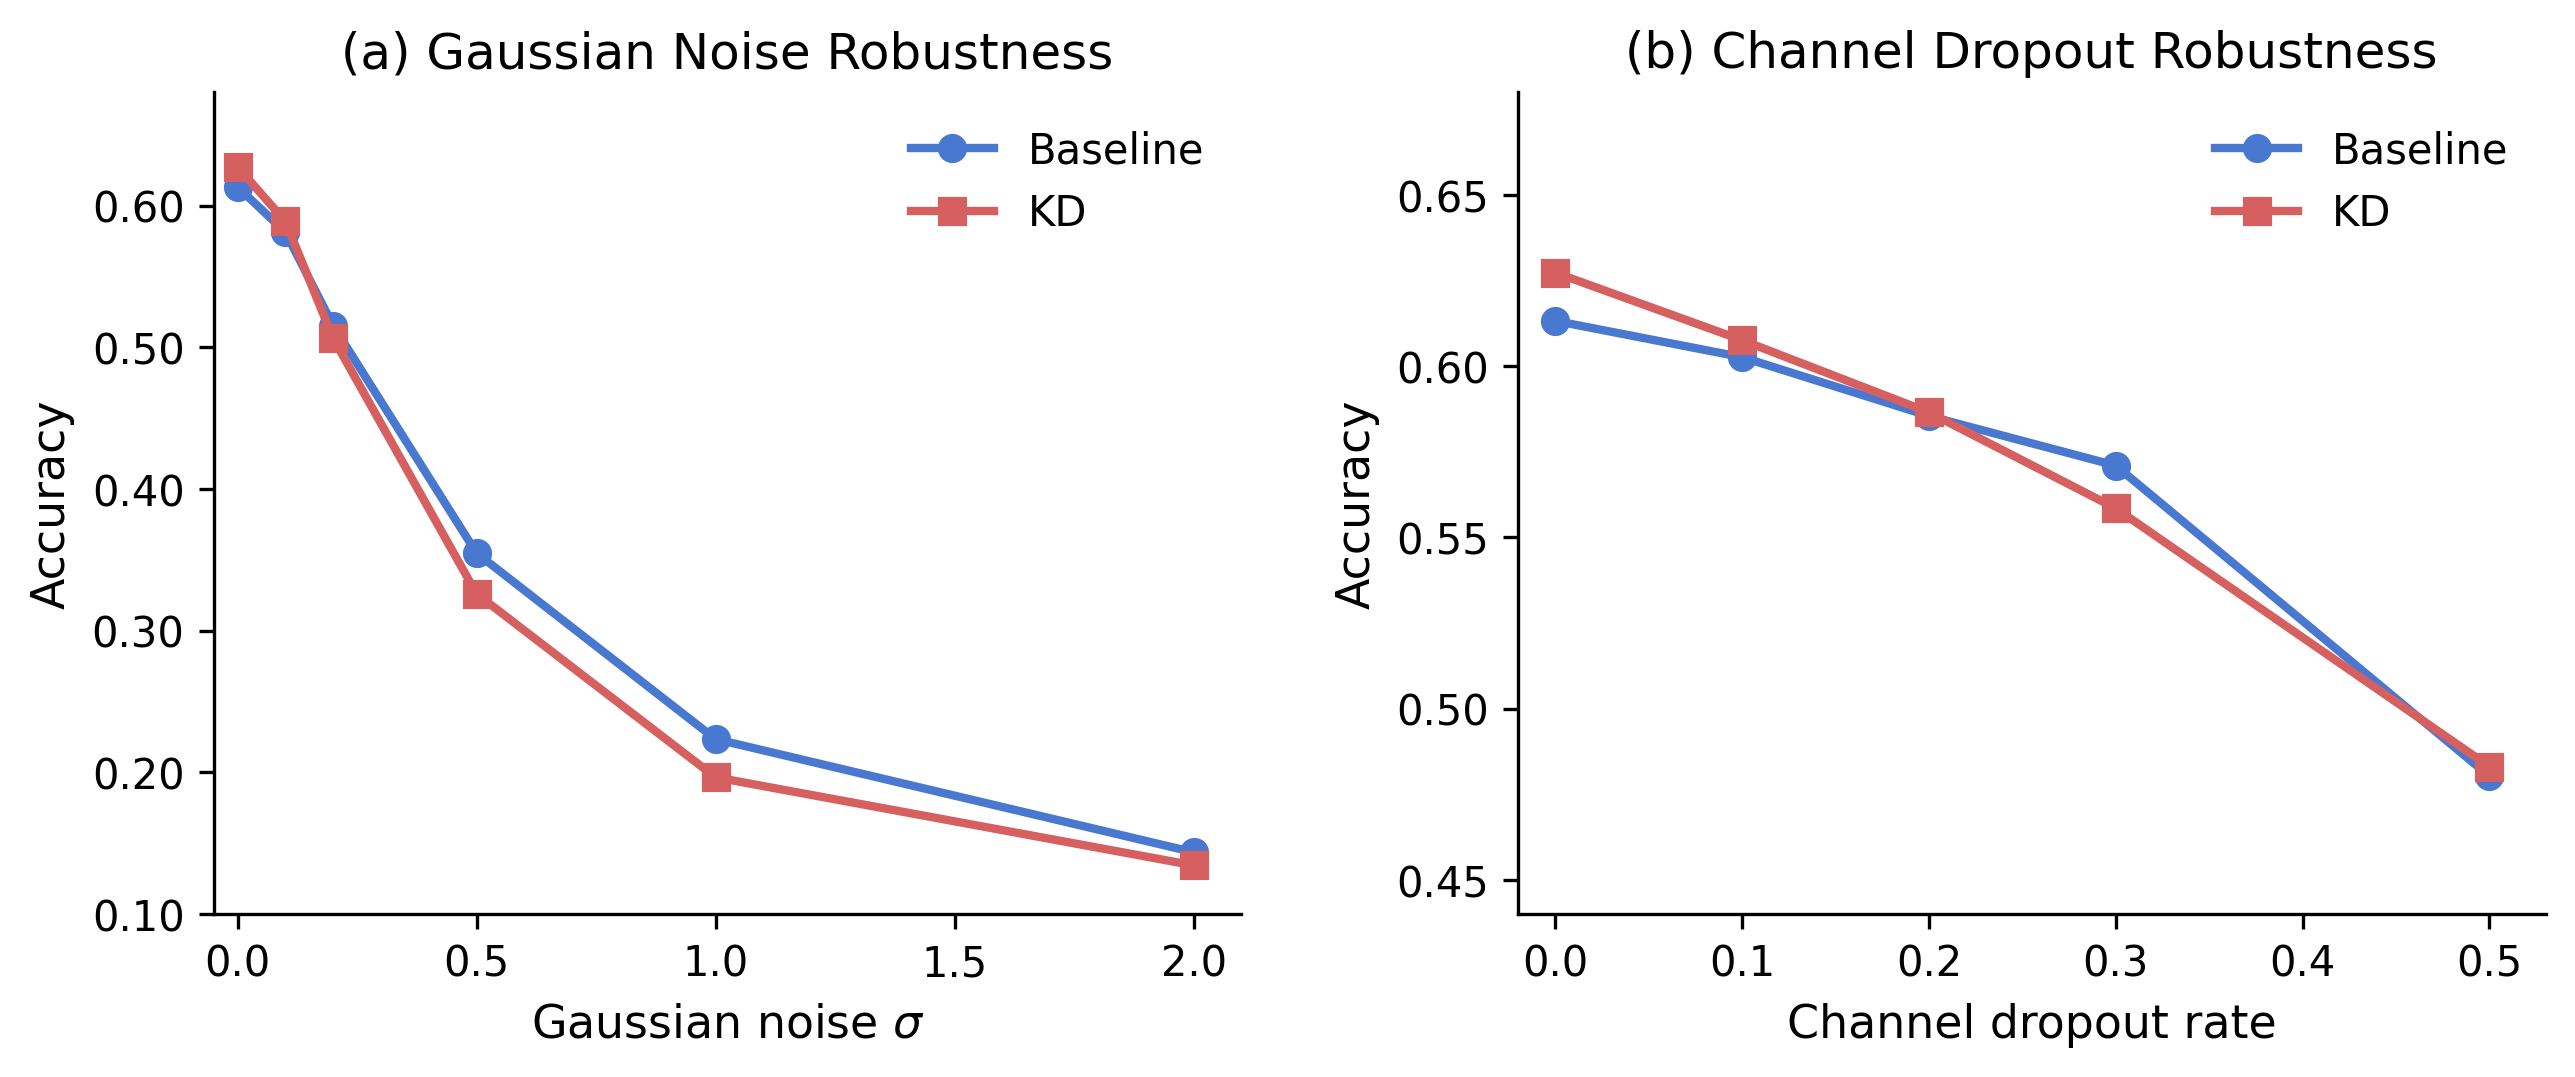
\includegraphics[width=\linewidth]{figs/fig_noise_robustness.png}
    \caption{Noise robustness comparison. \textbf{Left:} Accuracy under increasing Gaussian noise. KD is more robust at low noise ($\sigma \leq 0.1$) but degrades faster at higher noise levels. \textbf{Right:} Accuracy under channel dropout. Both models degrade similarly, with KD marginally better at low dropout rates.}
    \label{fig:noise_robustness}
\end{figure}

\subsection{Statistical Robustness via Bootstrap CIs}
\label{sec:bootstrap}
\vspace{-1mm}

\begin{table}[!t]
\caption{Bootstrap 95\% confidence intervals (10{,}000 resamples) for the main paired comparisons in this paper. CIs that exclude zero indicate effects that are reliable beyond the assumptions of paired $t$-tests. All comparisons are paired across 5 seeds.}
\small
\centering
\begin{tabular}{lcccc}
\toprule
Comparison & $\Delta$ mean & 95\% CI & $t$ & $p$ \\
\midrule
\rowcolor{blond}
\textbf{CBraMod FACED KD vs Baseline} & $\mathbf{+0.052}$ & $[+0.046, +0.057]$ & $15.5$ & $\mathbf{1{\times}10^{-4}}$ \\
\rowcolor{blond}
\textbf{LaBraM FACED KD vs Baseline} & $\mathbf{+0.026}$ & $[+0.011, +0.037]$ & $3.5$ & $\mathbf{0.025}$ \\
LaBraM SEED-V 19ch$\times$5\,s KD vs Base & $+0.018$ & $[+0.008, +0.028]$ & $3.1$ & $\mathbf{0.037}$ \\
CBraMod SEED-V 5\,s KD vs Base & $+0.0036$ & $[+0.0001, +0.0074]$ & $1.8$ & --- \\
Qwen-1.5B vs 0.5B (mid-layer KD) & $+0.015$ & $[+0.006, +0.024]$ & $2.8$ & $\mathbf{0.047}$ \\
\bottomrule
\end{tabular}
\label{tab:bootstrap}
\end{table}

\cref{tab:bootstrap} reports bootstrap 95\% percentile confidence intervals for all key comparisons in this paper. Bootstrap CIs are robust to non-normality of the seed-level differences and complement our paired $t$-tests. The two headline cross-backbone results (CBraMod FACED, LaBraM FACED) have CIs far from zero. The cross-dataset SEED-V results show CIs that exclude zero on both backbones, confirming that the framework generalizes.

\subsection{Computational Efficiency}
\label{sec:efficiency}
\vspace{-1mm}

CBraMod's backbone is 4.88M parameters (matching the published spec~\cite{wang2025cbramod}), and the classifier head is $128.4$M. KD adds a training-only semantic projection head ($+0.83$M) with \emph{zero inference overhead}---the semantic head is dropped at test time. Adapter64 adds $0.31$M adapter parameters and freezes the 4.88M backbone, preserving its pretrained features. The narrative for adapter PEFT in this setting is therefore one of \emph{feature preservation}: the frozen backbone retains its TUEG-pretrained representations intact while the adapters provide task-specific residual paths. Full parameter and inference-cost breakdown is reported in \cref{tab:supp_efficiency} (Supp.~\cref{sec:supp_efficiency}).
